\cotefile{154}
\scanpage{1}
\figure{%
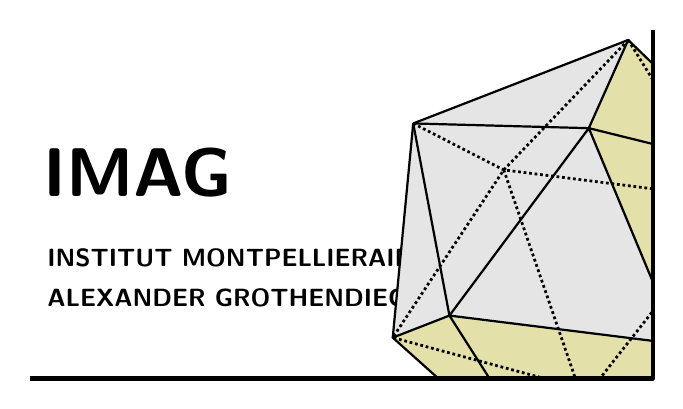
\begin{tikzpicture}[x=1cm,y=1cm,line join=round]
\node[anchor=west,font=\sffamily\bfseries\fontsize{48}{48}\selectfont] at (.15,2.85) {IMAG};
\node[anchor=west,font=\sffamily\bfseries\fontsize{9}{11}\selectfont] at (.20,1.77) {INSTITUT MONTPELLIERAIN};
\node[anchor=west,font=\sffamily\bfseries\fontsize{9}{11}\selectfont] at (.20,1.26) {ALEXANDER GROTHENDIECK};
\fill[gray!20] (4.97,3.48)--(7.70,4.54)--(7.20,3.42)--(8.00,1.50)--(8.00,.72)--(7.72,.44)--(5.43,1.04)--(4.71,.76)--cycle;
\fill[olive!25] (7.70,4.54)--(8.01,4.24)--(8.01,.24)--(5.29,.24)--(4.71,.76)--(5.43,1.04)--(8.00,.72)--(8.00,1.50)--(7.20,3.42)--cycle;
\draw[line width=.8pt] (4.71,.76)--(4.97,3.48)--(7.70,4.54)--(8.01,4.24);
\draw[line width=.8pt] (4.97,3.48)--(7.20,3.42)--(8.01,3.22) (7.70,4.54)--(7.20,3.42)--(5.43,1.04)--(4.71,.76)--(5.29,.24) (4.97,3.48)--(5.43,1.04)--(5.94,.24) (5.43,1.04)--(8.00,.72) (7.20,3.42)--(8.00,1.50);
\draw[densely dotted,line width=1pt] (4.97,3.48)--(6.12,2.89)--(8.01,2.65) (7.70,4.54)--(6.12,2.89)--(4.71,.76)--(6.64,.24) (6.12,2.89)--(7.03,.24) (7.70,4.54)--(8.01,4.04) (8.00,1.08)--(7.34,.24);
\draw[line width=1.5pt] (.10,.24)--(8.01,.24)--(8.01,4.67);
\end{tikzpicture}%
}

\scanpage{2}
\margin{\uline{18.1.84}}
\mspage{1}
Conventions particulières et constructions relatives aux pos. rel. supersingulières. \unsure{Quatre} possibilités:

\margin{\uuline{Les 5 variantes de la \unsure{notion} de déploiement d'un syst. de pseudo-droites}}

1) On n'admet pas les p.r. supersing. parmi les sommets du graphe du départ, i.e. comme définissant des faces de $\mathcal X$.
On trouve une surface $\mathcal X_0$ dans laquelle les ``pos. rel. supersingulières'' correspondent \deleted{aux}\inserted{à un} ``\unsure{sommet|sommets} \unsure{supersingulier|supersinguliers}'' --- ce sont les seuls sommets qui sont d'ordre $4n$, au lieu d'être d'ordre $4$.

\margin{\uline{NB} Il n'y a pas de ``bouts libres'' (rouges) en un sommet supersingulier --- toute \deleted{droite} ps.dr. aboutissant (comme une face $\unsure{F_i|F}$ incidente à $s$) en $s$, se prolonge sur la face antipodique $\unsure{F'|F'_i}$, \unsure{à} $F$ en $s$)}
\figure{%
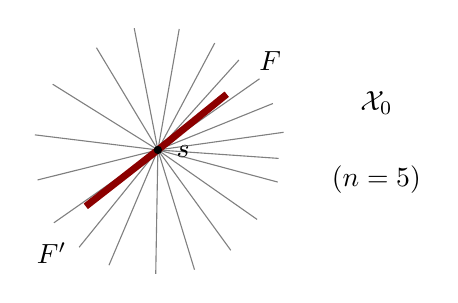
\begin{tikzpicture}[scale=.75]
\foreach \a/\r in {8/2.15,22/2.1,35/2.1,48/2.05,62/2.05,80/2.08,101/2.1,121/2.02,148/2.1,173/2.1,194/2.1,215/2.15,231/2.12,247/2.12,269/2.1,287/2.12,306/2.1,325/2.05,345/2.1,356/2.05}{\draw[gray] (0,0)--(\a:\r);}
\draw[red!55!black,line width=2.5pt] (39:1.5)--(0,0)--(218:1.55);
\fill (0,0) circle(2pt);\node[right] at (.15,-.03) {$s$};
\node at (1.9,1.5) {$F$};\node at (-1.8,-1.75) {$F'$};
\node at (3.7,.8) {$\mathcal X_0$};\node at (3.7,-.5) {$(n=5)$};
\end{tikzpicture}%
}

2) \deleted{Enfin}\inserted{On} admet les p.r. supersingulières comme \inserted{sommets} et les spécialisations directes (à partir d'une p.r. \uline{sous-stable}) vers celles-ci comme arêtes (correspondant, pour les p.r. sous-stables envisagées, à certains \uline{arcs de spécialisations} exceptionnels.
Finalement, il y a intérêt à les choisir aussi courts que possible (alors qu'au début je les choisissais aussi longs que possible), savoir de longueur combinatoire $1$, et placés à égale distance entre les arcs de transition (ou plutôt, de générisation) les plus proches). Ainsi, autour de la face supersingulière $F_i$ correspondant à une p.r. de générisation donnée, vont se raccorder (\deleted{\unsure{2n}}\inserted{le long de} $2(n-1)$ arcs de longueur combinatoire $1$ alors que) les $2(n-1)$ faces correspondant aux \unsure{\deleted{des}\inserted{positions}} relatives sous-stables proches, sans compter les \deleted{positions relatives}\inserted{(faces de) \unsure{biangles}}, stables proches, qui sont \deleted{\unsure{pris}} comprises \deleted{entre}\inserted{chacune entre} deux faces sous-stables avoisinantes, et touchant $F$ en \uline{un} sommet incident commun. Le nombre $2(n-1)$ est d'ailleurs correct, seulement dans le cas stable, dans le cas général c'est $2n_i$, où $n_i$ est le nb de sommets sur $D_i\unsure{\in|\subset}\Sigma_i$. Sur la surface $\mathcal X_1$ obtenue, tous les

\figure{%
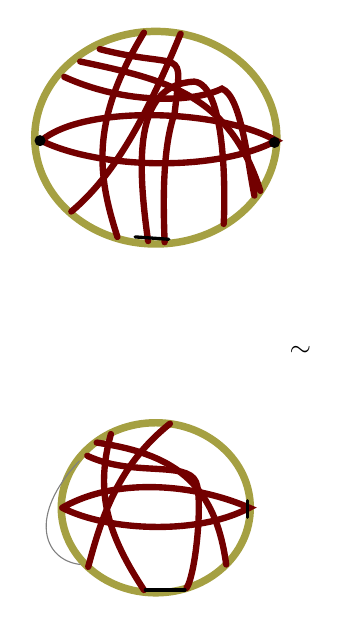
\begin{tikzpicture}[x=.75cm,y=.75cm,line cap=round]
\begin{scope}[yshift=4.7cm]
\draw[yellow!60!black,line width=2.7pt] (0,0) ellipse(2.05 and 1.8);
\draw[red!45!black,line width=2.3pt] (-1.94,-.05)..controls(-1.2,.57)and(1.1,.48)..(2.04,-.05)..controls(1,-.6)and(-1,-.52)..(-1.94,-.05);
\draw[red!45!black,line width=2.3pt] (-.2,1.78)..controls(-1.1,.3)and(-1.0,-.6)..(-.65,-1.68) (.42,1.76)..controls(-.1,.5)and(-.65,-.6)..(-1.43,-1.25);
\draw[red!45!black,line width=2.3pt] (-1.28,1.29)..controls(.2,.98)and(1.25,.72)..(1.77,-.9) (-1.55,1.03)..controls(-.5,.55)and(.66,.6)..(1.12,.83)..controls(1.45,.7)and(1.55,-.4)..(1.67,-.98);
\draw[red!45!black,line width=2.3pt] (-.95,1.5)..controls(.5,1.13)and(.45,1.6)..(.32,.42)..controls(.12,-.15)and(.12,-1.0)..(.15,-1.77) (-.13,-1.75)..controls(-.35,-.2)and(-.3,.9)..(.65,.95)..controls(1.18,.9)and(1.18,-.9)..(1.15,-1.46);
\draw[very thick] (-.35,-1.68)--(.22,-1.72);
\fill(-1.96,-.05)circle(2pt);\fill(2.01,-.08)circle(2pt);
\end{scope}
\node at (2.45,2.65) {$\unsure{\sim}$};
\begin{scope}[scale=.8]
\draw[yellow!60!black,line width=2.7pt] (0,0) ellipse(2 and 1.8);
\draw[red!45!black,line width=2.3pt] (-1.98,0)..controls(-.8,.68)and(.9,.48)..(1.98,0)..controls(.9,-.58)and(-1,-.5)..(-1.98,0);
\draw[red!45!black,line width=2.3pt] (-.95,1.56)..controls(-1.3,.3)and(-1,-.6)..(-.25,-1.74) (.3,1.78)..controls(-.8,.9)and(-1.15,-.2)..(-1.43,-1.25);
\draw[red!45!black,line width=2.3pt] (-1.45,1.1)..controls(-.5,.65)and(.65,1.0)..(.85,.55)..controls(1,.2)and(.85,-1.4)..(.65,-1.7);
\draw[red!45!black,line width=2.3pt] (-1.25,1.38)..controls(.3,1.15)and(1.25,.6)..(1.49,-1.2);
\draw[gray] (-1.62,.99)..controls(-2.7,-.15)and(-2.4,-1.1)..(-1.6,-1.2);
\draw[very thick] (-.22,-1.74)--(.62,-1.74);\draw[very thick](1.94,.15)--(1.94,-.2);
\end{scope}
\end{tikzpicture}%
}
\figure{%
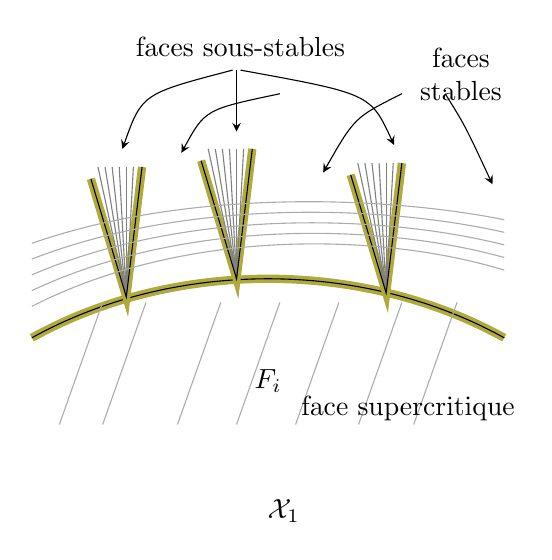
\begin{tikzpicture}[x=1cm,y=1cm,>=stealth]
\draw[yellow!65!black,line width=3pt] (-3,0)..controls(-1.2,1)and(1.2,1)..(3,0);
\draw[black] (-3,0)..controls(-1.2,1)and(1.2,1)..(3,0);
\foreach \x/\y in {-1.8/.52,-.4/.75,1.5/.57}{
\draw[yellow!65!black,line width=3pt] (\x-.45,\y+1.5)--(\x,\y)--(\x+.2,\y+1.65);
\foreach \d in {-.36,-.27,-.18,-.09,0,.09}{\draw[gray,thin] (\x,\y)--(\x+\d,\y+1.65);}
\draw (\x-.45,\y+1.5)--(\x,\y)--(\x+.2,\y+1.65);}
\foreach \j in {1,2,3,4,5}{\draw[gray!65,thin] (-3,.2+\j*.2)..controls(-1,1.3+\j*.12)and(1.5,1.2+\j*.12)..(3,.7+\j*.16);}
\foreach \x in {-2.1,-1.55,-.6,.15,.9,1.7,2.4}{\draw[gray!65,thin] (\x,.45)--(\x-.55,-1.1);}
\node at (0,-.55) {$F_i$};\node[right] at (.3,-.9) {face supercritique};
\node at (-.35,3.7) {faces sous-stables};
\draw[->] (-.4,3.4)--(-.4,2.62);\draw[->](-.45,3.4)..controls(-1.6,3.1)..(-1.85,2.4);\draw[->](-.35,3.4)..controls(1.3,3.1)..(1.6,2.45);
\node[align=center] at (2.45,3.35) {faces\\stables};
\draw[->] (2.25,3.1)..controls(2.5,2.7)..(2.85,1.95);
\draw[->] (1.7,3.1)..controls(1.1,2.8)..(.7,2.1);
\draw[->] (.15,3.1)..controls(-.8,2.9)..(-1.1,2.35);
\node at (.2,-2.2) {$\mathcal X_1$};
\end{tikzpicture}%
}
\margin{1}

\scanpage{3}
\mspage{2}
sommets, y compris ceux \deleted{\unsure{des deux}}\inserted{incidents} aux faces supercritiques, sont d'ordre $4$ --- les sommets sur une telle face $F_i$ correspondent aux \inserted{$2n_i$} arêtes \unsure{simplement} incidentes de $D_i$. Pour l'étude des ``bouts libres'' créés, supposant pour fixer les idées $\Sigma$ stable, on trouve suivant la parité de $n$:

a) $n$ pair, alors chaque face sous-stable donne \uline{deux} bouts libres placés aux extrémités de l'arête d'incidence, et chaque face stable qui touche $F_i$ donne de plus un bout libre cela fait donc
\[
2(2(n-1))+2(n-1)=6(n-1)
\]
bouts libres, ça fait un peu beaucoup.

b) $n$ impair, alors on trouve que chaque face sous-stable adjacente $1$ bout libre (au milieu de l'arête incidente commune), et $0$ sur les faces stables \unsure{juxtaincidentes}, en tout donc $2(n-1)$ bouts libres --- c'est juste ce qu'il faut pour espérer les raccorder, de façon à avoir \inserted{exactement} une des cartes de $(X,\Sigma)$ ``Affinisé'' par $D_i$.

\margin{\uline{NB} Pour le raccord de la face supercritique avec les faces sous-stables adjacentes, on doit encore définir sur $\widetilde D_i$ \deleted{des} (image inverse de $D_i$ dans $\widetilde X$) des \uline{arcs de générisation} \deleted{canoniques}\inserted{autour des} \deleted{les deux} sommets \deleted{\unsure{de}} $\widetilde D_i$, qu'on choisit de longueur combinatoire $1$ --- ce sont donc les arêtes de la subdivision cellulaire de $\widetilde D_i$ dont \unsure{ces celles données} par les les sommets. Non c'est mal dit, il vaut mieux prendre $\widetilde D_i$ \unsure{rev.} des vis de $D_i$, et définir l'arc de générisation rel\unsure{f} à une position relative sous-stable voisine de $D_i$, comme sur la figure ci-contre avec un arc de long $1$ équidistant des deux sommets sur $\widetilde D_i$ correspondant à $s$, et du côté où se trouve la p.r. $D$}
\figure{%
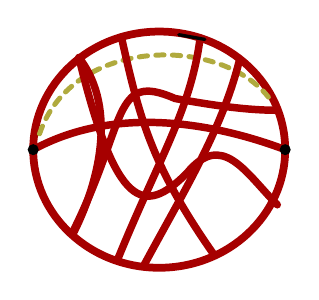
\begin{tikzpicture}[x=1cm,y=1cm,line cap=round]
\draw[red!65!black,line width=2.8pt] (0,0) ellipse(1.6 and 1.5);
\draw[yellow!65!black,dashed,line width=1.8pt] (-1.52,.2)..controls(-1.1,1.45)and(.8,1.45)..(1.4,.65);
\draw[red!65!black,line width=2.7pt] (-1.6,0)..controls(-.5,.6)and(.8,.3)..(1.6,0);
\draw[red!65!black,line width=2.7pt] (-1.02,1.17)..controls(-.5,.5)and(-.8,-.5)..(-1.1,-1.08) (-.48,1.43)..controls(-.25,.4)and(-.1,-.2)..(.7,-1.34) (.52,1.42)..controls(.4,.5)and(.0,-.1)..(-.53,-1.4) (1.02,1.14)..controls(.8,.25)and(.3,-.55)..(-.2,-1.48);
\draw[red!65!black,line width=2.7pt] (-1.1,-1.05)..controls(-.4,.35)and(-.6,1)..(.2,.65)..controls(.75,.55)and(1.15,.5)..(1.5,.5);
\draw[red!65!black,line width=2.7pt] (-1.02,1.17)..controls(-.55,-.75)and(-.2,-.85)..(.35,-.3)..controls(.8,.25)and(1.1,-.3)..(1.5,-.7);
\fill(-1.6,0)circle(2pt);\fill(1.6,0)circle(2pt);\draw[very thick](.25,1.46)--(.58,1.4);
\end{tikzpicture}%
}

Le cas $n$ impair est satisfaisant, mais pas le cas pair tel quel, car il y a alors redondance des bouts libres. Une façon de s'en tirer dans tous les cas, c'est de \deleted{\unsure{partir}}\inserted{partir de} la carte $\mathcal X_0$, et de la modifier en remplaçant chaque sommet supercritique $s$ par un petit disque supercritique.
\deleted{Le nb} Dans le cas $n$ \unsure{pair} chaque face sous-stable incidente à $s$ contribue $\unsure{1|0}$ bout libre, et chaque face stable incidente $1$ bout, et c'est l'inverse si $n$ est impair, donc en tout il y aura $2(n-1)$ bouts libres \deleted{\unsure{et}} qui aboutissent en $F_s$, et \deleted{\unsure{si je raccorde les bouts}}\inserted{le polygone combinatoire qu'ils forment est} can. hom. à celui obtenu sur $\widetilde D_i$ --- d'où une
\margin{2}

\scanpage{4}
\mspage{3}
façon particulièrement jolie de les raccorder, de façon à reconstituer \deleted{une}\inserted{l'}affinisation supercritique de $\underline\Sigma$ sur $F_i$. On trouve une surface $\mathcal X'_1$, où les sommets \deleted{\unsure{supercri}}\inserted{sur les} faces supersingulières sont d'ordre $3$, tous les autres sommets étant d'ordre $4$. Il faudrait expliciter les arcs de spécialisation (et \unsure{aussi|non}, symétriquement, de générisation sur les $\widetilde D_i$), non seulement sur les p.r. sous-stables voisines de $D_i$, mais maintenant aussi sur les p.r. stables voisines. Cette fois, on a des arcs de spécialisation de longueur combinatoire $\frac12$ --- ce qui amène à introduire la subdivision barycentrique \unsure{itérée double} de la subdivision cellulaire qu'on a sur les $\widetilde D$ et les $\widetilde D_i$. \deleted{Et}

\figure{%
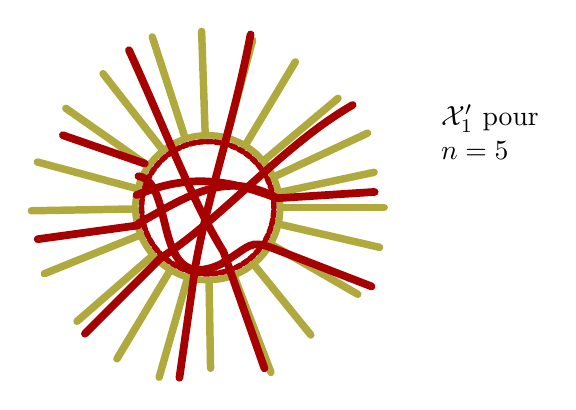
\begin{tikzpicture}[scale=.8,line cap=round]
\draw[yellow!65!black,line width=2.4pt](0,0)circle(1.15);
\foreach \a/\r in {0/2.8,12/2.7,25/2.8,40/2.7,59/2.7,75/2.75,92/2.8,108/2.85,128/2.7,145/2.75,165/2.8,181/2.8,202/2.8,221/2.75,239/2.8,254/2.8,271/2.55,291/2.8,309/2.6,330/2.75,347/2.8}{\draw[yellow!65!black,line width=2.7pt](\a:1.15)--(\a:\r);}
\draw[red!65!black,densely dotted,line width=2pt](0,0)circle(1.05);
\draw[red!65!black,line width=2.8pt] (-1.13,.2)..controls(-.4,.5)and(.2,.5)..(1.1,.15)--(2.65,.25) (-1.1,-.28)--(-2.7,-.5);
\draw[red!65!black,line width=2.8pt] (-1.1,-.25)..controls(-.3,.2)and(.3,.6)..(1.1,.15);
\draw[red!65!black,line width=2.8pt] (-1.25,2.5)..controls(-.7,1.3)and(-.25,.1)..(.25,-.7)--(.9,-2.55);
\draw[red!65!black,line width=2.8pt] (.68,2.75)..controls(.4,1.3)and(.0,.2)..(-.2,-.95)--(-.45,-2.7);
\draw[red!65!black,line width=2.8pt] (2.3,1.63)..controls(1.2,1)and(.2,-.2)..(-.75,-.8)--(-1.95,-2.0);
\draw[red!65!black,line width=2.8pt] (-1.1,.5)..controls(-.5,.4)and(-.9,-1.4)..(.2,-.9)..controls(.7,-.6)and(.65,-.5)..(1.05,-.65)--(2.6,-1.25);
\draw[red!65!black,line width=2.8pt](-2.3,1.15)--(-1.0,.7);
\node[right,align=left]at(3.55,1.2){$\mathcal X'_1$ pour\\$n=5$};
\end{tikzpicture}%
}

Le défaut commun \deleted{aux}\inserted{à ces} trois surfaces représentatives $\mathcal X_0$, $\mathcal X_1$, $\mathcal X'_1$ pour les p.rel. est que le système local, ou transport parallèle, des \deleted{$\unsure{D}$} \unsure{polygônes|polygones} combinatoires $\operatorname{Pol}(D)$ n'est défini ici que sur le complémentaire de l'union des \deleted{\unsure{faces}}\inserted{sommets}, ou faces supercritiques, qui sont des lieux de ramification effective.
Un autre défaut, sans doute apparenté, est qu'on n'a pas d'\unsure{application|injection} naturelle de ces surfaces dans $X$, sauf erreur (\deleted{sauf erreur} peut-être dans le cas de $\mathcal X'_1$ --- à regarder de façon \deleted{plus} détaillée\ldots). C'est pour pallier à ce (ou ces) défauts qu'il peut être
\margin{3}

\scanpage{5}
\mspage{4}
utile d'introduire d'autres variantes.

3) \deleted{\unsure{S}} Surface obtenue comme $\mathcal X_0$ en excluant les p.r. super\deleted{singulières}\inserted{critiques}, mais en introduisant, pour éviter les sommets supercritiques, des arêtes supplémentaires du graphe \inserted{$\Gamma$} des p.r., savoir les ``balayages au-dessous d'une p.r. supercritique'' \inserted{$D_i$}, et ceci aussi bien pour une p.r. voisine sous-stable, que stable. Cela fait donc des arcs de transition supplémentaires, qui \deleted{\unsure{remplacent}}\inserted{prennent} la place des arcs de spéc. supercritique de $2^\circ$, mais qui ne sont plus des arcs de spécialisation, à proprement parler. Et d'ailleurs l'opération correspondante doit être considérée comme étant \uline{de poids $2$}, et non $1$ comme les autres.
\figure{%
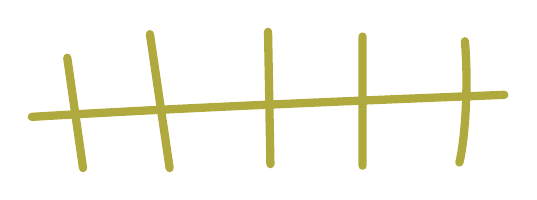
\begin{tikzpicture}[x=1cm,y=1cm,line cap=round]
\draw[yellow!65!black,line width=3pt] (-3,0)..controls(-1,.12)and(1,.2)..(3,.28);
\draw[yellow!65!black,line width=3pt] (-2.55,.75)--(-2.35,-.65) (-1.5,1.05)--(-1.25,-.65) (.0,1.08)--(.03,-.6) (1.2,1.02)--(1.2,-.62) (2.5,.96)..controls(2.55,.4)and(2.5,-.3)..(2.43,-.58);
\end{tikzpicture}%
}
On trouve, dans la surface $\mathcal X_2$ obtenue, \deleted{et} (décomposée \inserted{cellulairement} par le graphe dual de $\Gamma$) des sommets qui à nouveau sont tous d'ordre $4$, ils \inserted{(ceux qui sont proches \deleted{\unsure{à}} $D_i$)} correspondent aux \deleted{\unsure{triplets de deux arêtes}} \inserted{paires $(s,a)$ où $s$ \unsure{sommet de} $D_i$, $a$ arête sur $D_i$ incidents} de $D_i$ \deleted{\unsure{d'une arête}\illegible{3}\unsure{adjacentes}}, i.e. aux arêtes de la subdivision barycentrique \deleted{de $\unsure{X}$} de $D_i$, il y en a $2(n-1)$ dans le cas stable.
Si je me rappelle bien, $D_i$ est plongée dans $\mathcal X_3$, de faç que les sommets de la \deleted{\unsure{subdivision}}\inserted{décomposition} cell. de $D_i$ double de la subd. bar. de celle qu'on a au départ, \deleted{\unsure{tous}} correspondent à des sommets de $\mathcal X_3$.
\margin{4}

\scanpage{6}
\margin{5}
\texttt{//*\quad CRAY2\quad 0429\qquad \unsure{I|1}}
\figure{%
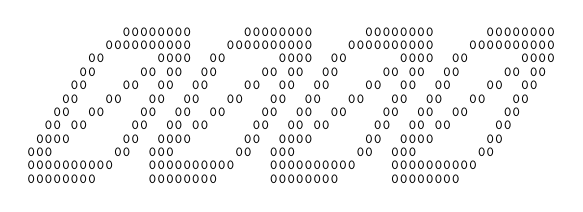
\begin{tikzpicture}[x=.11cm,y=.17cm]
\foreach \x/\y in {11/0,12/0,13/0,14/0,15/0,16/0,17/0,18/0,9/-1,10/-1,11/-1,12/-1,13/-1,14/-1,15/-1,16/-1,17/-1,18/-1,7/-2,8/-2,15/-2,16/-2,17/-2,18/-2,6/-3,7/-3,13/-3,14/-3,16/-3,17/-3,5/-4,6/-4,11/-4,12/-4,15/-4,16/-4,4/-5,5/-5,9/-5,10/-5,14/-5,15/-5,3/-6,4/-6,7/-6,8/-6,13/-6,14/-6,2/-7,3/-7,5/-7,6/-7,12/-7,13/-7,1/-8,2/-8,3/-8,4/-8,11/-8,12/-8,0/-9,1/-9,2/-9,10/-9,11/-9,0/-10,1/-10,2/-10,3/-10,4/-10,5/-10,6/-10,7/-10,8/-10,9/-10,0/-11,1/-11,2/-11,3/-11,4/-11,5/-11,6/-11,7/-11,25/0,26/0,27/0,28/0,29/0,30/0,31/0,32/0,23/-1,24/-1,25/-1,26/-1,27/-1,28/-1,29/-1,30/-1,31/-1,32/-1,21/-2,22/-2,29/-2,30/-2,31/-2,32/-2,20/-3,21/-3,27/-3,28/-3,30/-3,31/-3,19/-4,20/-4,25/-4,26/-4,29/-4,30/-4,18/-5,19/-5,23/-5,24/-5,28/-5,29/-5,17/-6,18/-6,21/-6,22/-6,27/-6,28/-6,16/-7,17/-7,19/-7,20/-7,26/-7,27/-7,15/-8,16/-8,17/-8,18/-8,25/-8,26/-8,14/-9,15/-9,16/-9,24/-9,25/-9,14/-10,15/-10,16/-10,17/-10,18/-10,19/-10,20/-10,21/-10,22/-10,23/-10,14/-11,15/-11,16/-11,17/-11,18/-11,19/-11,20/-11,21/-11,39/0,40/0,41/0,42/0,43/0,44/0,45/0,46/0,37/-1,38/-1,39/-1,40/-1,41/-1,42/-1,43/-1,44/-1,45/-1,46/-1,35/-2,36/-2,43/-2,44/-2,45/-2,46/-2,34/-3,35/-3,41/-3,42/-3,44/-3,45/-3,33/-4,34/-4,39/-4,40/-4,43/-4,44/-4,32/-5,33/-5,37/-5,38/-5,42/-5,43/-5,31/-6,32/-6,35/-6,36/-6,41/-6,42/-6,30/-7,31/-7,33/-7,34/-7,40/-7,41/-7,29/-8,30/-8,31/-8,32/-8,39/-8,40/-8,28/-9,29/-9,30/-9,38/-9,39/-9,28/-10,29/-10,30/-10,31/-10,32/-10,33/-10,34/-10,35/-10,36/-10,37/-10,28/-11,29/-11,30/-11,31/-11,32/-11,33/-11,34/-11,35/-11,53/0,54/0,55/0,56/0,57/0,58/0,59/0,60/0,51/-1,52/-1,53/-1,54/-1,55/-1,56/-1,57/-1,58/-1,59/-1,60/-1,49/-2,50/-2,57/-2,58/-2,59/-2,60/-2,48/-3,49/-3,55/-3,56/-3,58/-3,59/-3,47/-4,48/-4,53/-4,54/-4,57/-4,58/-4,46/-5,47/-5,51/-5,52/-5,56/-5,57/-5,45/-6,46/-6,49/-6,50/-6,55/-6,56/-6,44/-7,45/-7,47/-7,48/-7,54/-7,55/-7,43/-8,44/-8,45/-8,46/-8,53/-8,54/-8,42/-9,43/-9,44/-9,52/-9,53/-9,42/-10,43/-10,44/-10,45/-10,46/-10,47/-10,48/-10,49/-10,50/-10,51/-10,42/-11,43/-11,44/-11,45/-11,46/-11,47/-11,48/-11,49/-11}{\node[inner sep=0pt,font=\ttfamily\tiny] at (\x,\y) {0};}
\end{tikzpicture}%
}
\figure{%
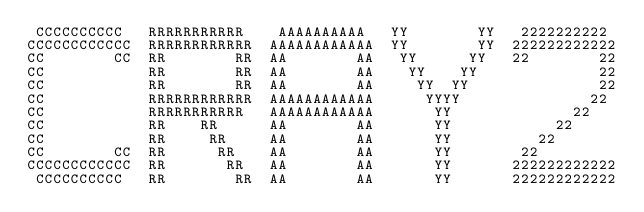
\begin{tikzpicture}[x=.11cm,y=.17cm]
\foreach \x/\y in {1/0,2/0,3/0,4/0,5/0,6/0,7/0,8/0,9/0,10/0,0/-1,1/-1,2/-1,3/-1,4/-1,5/-1,6/-1,7/-1,8/-1,9/-1,10/-1,11/-1,0/-2,1/-2,10/-2,11/-2,0/-3,1/-3,0/-4,1/-4,0/-5,1/-5,0/-6,1/-6,0/-7,1/-7,0/-8,1/-8,0/-9,1/-9,10/-9,11/-9,0/-10,1/-10,2/-10,3/-10,4/-10,5/-10,6/-10,7/-10,8/-10,9/-10,10/-10,11/-10,1/-11,2/-11,3/-11,4/-11,5/-11,6/-11,7/-11,8/-11,9/-11,10/-11}{\node[inner sep=0pt,font=\ttfamily\tiny] at (\x,\y) {C};}
\foreach \x/\y in {14/0,15/0,16/0,17/0,18/0,19/0,20/0,21/0,22/0,23/0,24/0,14/-1,15/-1,16/-1,17/-1,18/-1,19/-1,20/-1,21/-1,22/-1,23/-1,24/-1,25/-1,14/-2,15/-2,24/-2,25/-2,14/-3,15/-3,24/-3,25/-3,14/-4,15/-4,24/-4,25/-4,14/-5,15/-5,16/-5,17/-5,18/-5,19/-5,20/-5,21/-5,22/-5,23/-5,24/-5,25/-5,14/-6,15/-6,16/-6,17/-6,18/-6,19/-6,20/-6,21/-6,22/-6,23/-6,24/-6,14/-7,15/-7,20/-7,21/-7,14/-8,15/-8,21/-8,22/-8,14/-9,15/-9,22/-9,23/-9,14/-10,15/-10,23/-10,24/-10,14/-11,15/-11,24/-11,25/-11}{\node[inner sep=0pt,font=\ttfamily\tiny] at (\x,\y) {R};}
\foreach \x/\y in {29/0,30/0,31/0,32/0,33/0,34/0,35/0,36/0,37/0,38/0,28/-1,29/-1,30/-1,31/-1,32/-1,33/-1,34/-1,35/-1,36/-1,37/-1,38/-1,39/-1,28/-2,29/-2,38/-2,39/-2,28/-3,29/-3,38/-3,39/-3,28/-4,29/-4,38/-4,39/-4,28/-5,29/-5,30/-5,31/-5,32/-5,33/-5,34/-5,35/-5,36/-5,37/-5,38/-5,39/-5,28/-6,29/-6,30/-6,31/-6,32/-6,33/-6,34/-6,35/-6,36/-6,37/-6,38/-6,39/-6,28/-7,29/-7,38/-7,39/-7,28/-8,29/-8,38/-8,39/-8,28/-9,29/-9,38/-9,39/-9,28/-10,29/-10,38/-10,39/-10,28/-11,29/-11,38/-11,39/-11}{\node[inner sep=0pt,font=\ttfamily\tiny] at (\x,\y) {A};}
\foreach \x/\y in {42/0,43/0,52/0,53/0,42/-1,43/-1,52/-1,53/-1,43/-2,44/-2,51/-2,52/-2,44/-3,45/-3,50/-3,51/-3,45/-4,46/-4,49/-4,50/-4,46/-5,47/-5,48/-5,49/-5,47/-6,48/-6,47/-7,48/-7,47/-8,48/-8,47/-9,48/-9,47/-10,48/-10,47/-11,48/-11}{\node[inner sep=0pt,font=\ttfamily\tiny] at (\x,\y) {Y};}
\foreach \x/\y in {57/0,58/0,59/0,60/0,61/0,62/0,63/0,64/0,65/0,66/0,56/-1,57/-1,58/-1,59/-1,60/-1,61/-1,62/-1,63/-1,64/-1,65/-1,66/-1,67/-1,56/-2,57/-2,66/-2,67/-2,66/-3,67/-3,66/-4,67/-4,65/-5,66/-5,63/-6,64/-6,61/-7,62/-7,59/-8,60/-8,57/-9,58/-9,56/-10,57/-10,58/-10,59/-10,60/-10,61/-10,62/-10,63/-10,64/-10,65/-10,66/-10,67/-10,56/-11,57/-11,58/-11,59/-11,60/-11,61/-11,62/-11,63/-11,64/-11,65/-11,66/-11,67/-11}{\node[inner sep=0pt,font=\ttfamily\tiny] at (\x,\y) {2};}
\end{tikzpicture}%
}

\diagram{%
\begin{array}{llllllllllll}
\texttt{****A}&\texttt{START}&\texttt{JOB}&\texttt{429}&\texttt{CRAY2}&\texttt{ROOM}&\texttt{4.30.42 PM 16 AUG 82}&\texttt{R6.PR1}&\texttt{SYS JES2}&\texttt{JOB 429}&\texttt{START}&\texttt{A****}\\
\texttt{****A}&\texttt{START}&\texttt{JOB}&\texttt{429}&\texttt{CRAY2}&\texttt{ROOM}&\texttt{4.30.42 PM 16 AUG 82}&\texttt{R6.PR1}&\texttt{SYS JES2}&\texttt{JOB 429}&\texttt{START}&\texttt{A****}\\
\texttt{****A}&\texttt{START}&\texttt{JOB}&\texttt{429}&\texttt{CRAY2}&\texttt{ROOM}&\texttt{4.30.42 PM 16 AUG 82}&\texttt{R6.PR1}&\texttt{SYS JES2}&\texttt{JOB 429}&\texttt{START}&\texttt{A****}\\
\texttt{****A}&\texttt{START}&\texttt{JOB}&\texttt{429}&\texttt{CRAY2}&\texttt{ROOM}&\texttt{4.30.42 PM 16 AUG 82}&\texttt{R6.PR1}&\texttt{SYS JES2}&\texttt{JOB 429}&\texttt{START}&\texttt{A****}\\
\texttt{****A}&\texttt{START}&\texttt{JOB}&\texttt{429}&\texttt{CRAY2}&\texttt{ROOM}&\texttt{4.30.42 PM 16 AUG 82}&\texttt{R6.PR1}&\texttt{SYS JES2}&\texttt{JOB 429}&\texttt{START}&\texttt{A****}\\
\texttt{****A}&\texttt{START}&\texttt{JOB}&\texttt{429}&\texttt{CRAY2}&\texttt{ROOM}&\texttt{4.30.42 PM 16 AUG 82}&\texttt{R6.PR1}&\texttt{SYS JES2}&\texttt{JOB 429}&\texttt{START}&\texttt{A****}
\end{array}%
}
\texttt{DERNIERE MISE A JOUR DE JOURNAL : 11-08-82}

\texttt{ATTENTION ...........}

\texttt{1. ARRET DE L'ORDINATEUR LE MARDI 17 AOUT DE 7 H A 8 H.}

\diagram{%
\begin{array}{ll}
\texttt{]}&\texttt{2. UNE MODIFICATION SYSTEME NOUS CONTRAINDRA A DETRUIRE}\\
\texttt{]}&\quad\texttt{LE CONTENU DU DISQUE SPOOL LE MARDI 17 AOUT A 6 HEURES}\\
\texttt{]}&\quad\texttt{VEUILLEZ RECUPERER VOS SORTIES EN ATTENTE AVANT CETTE}\\
\texttt{]}&\quad\texttt{DATE. MERCI DE VOTRE COMPREHENSION.}\\
\texttt{]}&\texttt{3. UN ARRET EXCEPTIONNEL POUR PREPARER L'ARRIVEE DE NOUVELLES}\\
\texttt{]}&\quad\texttt{UNITES AURA LIEU DU VENDREDI 20 AOUT A 17H 30 AU LUNDI}\\
\texttt{]}&\quad\texttt{23 AOUT A \unsure{9H|3H}.}
\end{array}%
}

\scanpage{7}
\mspage{5}
Cette carte \inserted{$\mathcal X_2$} est déduite de $\mathcal X_0$ en faisant ``éclater'' les \deleted{\unsure{p}} sommets supersinguliers, ou encore de $\mathcal X_1$ en découpant \inserted{l'int.} des faces supersingulières et en identifiant des pts antipodiques sur leurs bords. --- ce qui explicite aussi la façon dont les $D_i$ sont plongés dans $\mathcal X$. Cette fois, on a une carte où toutes les faces peuvent être considérées comme \inserted{des $\unsure{\square}$} \deleted{d'}ordre \deleted{$\unsure{2n}$} $(4n)$, où tous les sommets d'ordre pair (et $=$ d'ordre $4$). Sur cette carte, les $\operatorname{Pol}(D)$ forment un syst. local (\deleted{mais} --- alors que sur $\mathcal X_0$, c'est ramifié (avec \uline{indice de ramification $n$}) autour de chaque sommet. Quant aux bouts libres, de part et d'autre de $D_i\subset\mathcal X$, ils se raccordent de façon satisfaisante encore. Cette carte d'autre part ne s'envoie \uline{pas} dans $X$ (sauf erreur).

\margin{\figure{%
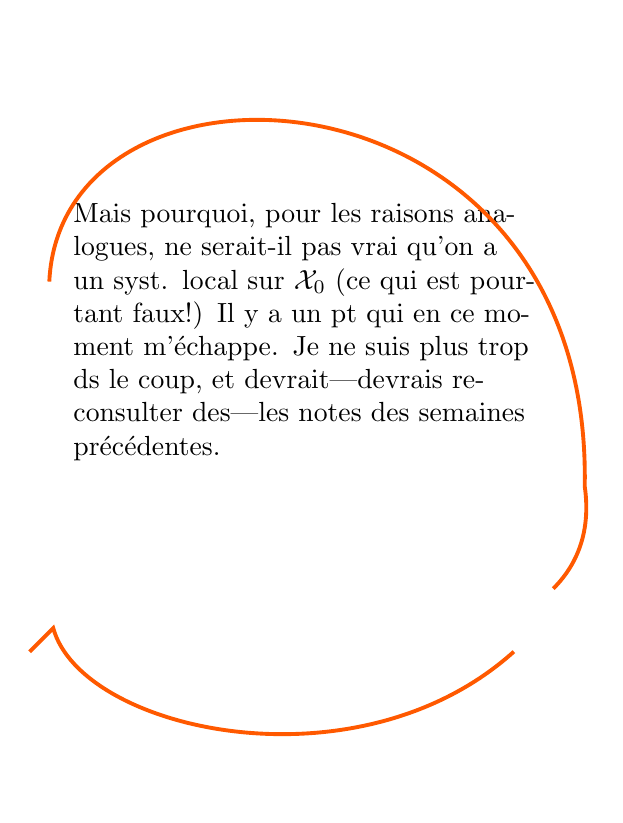
\begin{tikzpicture}[x=1cm,y=1cm]
\node[anchor=north west,text width=6.1cm,align=left,inner sep=0pt] at (0,0) {Mais pourquoi, pour les raisons analogues, ne serait-il pas vrai qu'on a un syst. local sur $\mathcal X_0$ (ce qui est pourtant faux!) Il y a un pt qui en ce moment m'échappe. Je ne suis plus trop ds le coup, et \unsure{devrait|devrais} reconsulter \unsure{des|les} notes des semaines précédentes.};
\draw[orange!70!red,line width=1.4pt] (-.3,-1)..controls(-.15,2.2)and(6.6,1.9)..(6.5,-3.6)..controls(6.6,-4.3)and(6.3,-4.7)..(6.1,-4.9);
\draw[orange!70!red,line width=1.4pt] (5.6,-5.7)..controls(3.6,-7.5)and(.1,-6.7)..(-.25,-5.4)--(-.55,-5.7);
\end{tikzpicture}%
}}

4) Ce dernier inconvénient n'est pas présent pour la carte $\mathcal X_3$, qui \deleted{est} par ailleurs
\margin{6}

\scanpage{8}
\texttt{/*JOB=CRAY2,ACCT=*********,ALL=M06,MSGL=N}\qquad\texttt{J0429CNU}

\texttt{// JOB MSGLEVEL=(1,1),MSGCLASS=A}

\texttt{// EXEC PGM=IEFBR14}
\margin{7}

\scanpage{9}
\mspage{6}

ressemble d'assez près à $\mathcal X_2$ (les surfaces sous-jacentes sont homéom., \unsure{tout} comme les surfaces sous-jacentes $\mathcal X_0,\mathcal X_1,\mathcal X'_1$ le sont entre elles). On l'obtient en \deleted{\unsure{ajoutant}}\inserted{admettant} les positions relatives super\deleted{singulières}\inserted{critiques} parmi les faces admises, mais en \deleted{prenant \illegible{1}}\inserted{considérant}, pour une $D_i$ fixée ayant $n_i$ sommets, $2n_i$ positions relatives supercritiques \inserted{$D'_i$} correspondantes, suivant la position du pt d'intersection virtuel $D_i\cap D'_i$, qui doit être sur une des $2n_i$ facettes sur $\unsure{\widetilde D_i|\widehat D_i}$.

On trouve encore que tous les sommets sont d'ordre $4$. La \deleted{\unsure{ps.dr.}} ps. droite $D_i\subset\mathcal X_2$ est ici remplacée par une \deleted{\unsure{collier}\ \illegible{1}}\inserted{bande (de Möbius)} de $D_i$. Cela revient, à partir de $\mathcal X'_1$, \deleted{au lieu} \deleted{alors}\inserted{après} avoir découpé les faces supercritiques, au lieu d'identifier directement des pts antipodiques de chaque comp. conn. du bord, \deleted{de}\inserted{à} \deleted{prendre}\inserted{\unsure{fixer}} d'abord \deleted{\unsure{une}} une ``virole'' à ce bord \unsure{par un} bord, qui délimite cette bande de Möbius.

Cette fois on aura une application $\mathcal X_3\mathbin{-}X$, telle que l'image inverse de $X_1$ soit ce qu'il faut, \deleted{Mais} y compris les $D_i$ de \unsure{tout à l'h.} Mais on notera que sur les faces \inserted{supercritiques} de $\mathcal X_3$, il n'y a pas cette fois-ci de représentation affinisée de $\underline\Sigma=(X,\Sigma)$ comme dans le cas de $\mathcal X'_1$, \deleted{mais} plutôt une représentation d'une partie pertinente d'un voisinage tubulaire conv. de $D_i$ dans $X$.

D'autre part, les \deleted{\unsure{7}} faces supersingulières ne sont pas de $=$ \deleted{ordre que} les autres, de sorte que $\mathcal X_3$ ne se prête pas à une interprétation, en termes de la combinatoire interne, du syst. local des $\operatorname{Pol}(D)$.

\margin{\uline{TSVP}}
\margin{8}

\scanpage{10}
\mspage{$6'$}

En plus de ces $5$ variantes $\mathcal X_0,\mathcal X_1,\mathcal X'_1,\mathcal X_2,\mathcal X_3$ il y a \inserted{bien entendu} les revêtements de ces cartes (ramifiés pour les trois premières) principaux de groupe $D_{2n}$, associés aux $\operatorname{Pol}(D)$. Ce sont les revêtements $\widetilde{\mathcal X}_i$ qui sont les déploiements ultimes.

Les surfaces les plus utiles me semblent ici $\mathcal X'_1,\mathcal X_2,\mathcal X_3$ et leurs revêtements $\widetilde{\mathcal X}'_1,\widetilde{\mathcal X}_2,\widetilde{\mathcal X}_3$. Peut-être peut-on se passer des $\mathcal X_2,\mathcal X_3$ et leurs tildés, au profit des $\overset{\deleted{\unsure{\sim}}}{\mathcal X}'_1$ et $\widetilde{\mathcal X}'_1$, d'autant que $\mathcal X'_1$ s'envoie bien dans $X$ comme prévu --- je \inserted{ne} suis pas tout à fait \unsure{convaincu} des \unsure{collisions|collages}, \deleted{\unsure{ayant quelque}}\inserted{en usage} \unsure{qd}, comment ça se passe au voisinage du bord d'une face supercritique.

\margin{9}

\begin{tabular}{@{}l@{}}
\texttt{********************************************************************************}\\
\texttt{*JESNEWS\ DU\ 02/08/1982\ \unsure{C63|C68}\ CADARACHE\ \ \ \ \ \ \ \ \ \ \ \ \ \ \ \ \ \ \ \ \ \ \ \ \ \ \ \ \ \ \ \ \ \ \ \ \ \ \ \ \ \ \ \ \ *}\\
\texttt{********************************************************************************}\\
\texttt{*\ \ \ \ \ \ DEPUIS\ LE\ 1/7/82\ LES\ ALIAS\ DES\ COMMANDES\ LIBRARIAN\ \ \ \ \ \ \ \ \ \ \ \ \ \ \ \ \ \ \ \ \ \ *}\\
\texttt{*\ \ \ \ \ \ \ \ \ \ \ \ \ LIBGET\ (LG)\ ET\ LIBSAVE\ (LS)\ SONT\ SUPPRIMES,\ \ \ \ \ \ \ \ \ \ \ \ \ \ \ \ \ \ \ \ \ *}\\
\texttt{*\ \ \ \ \ \ \ \ \ \ \ \ \ POUR\ EVITER\ UNE\ POSSIBILITE\ DE\ CONFLIT\ AVEC\ \ \ \ \ \ \ \ \ \ \ \ \ \ \ \ \ \ \ \ *}\\
\texttt{*\ \ \ \ \ \ \ \ \ \ \ \ \ LE\ MEME\ ALIAS\ DES\ COMMANDES\ STANDARD\ IBM.\ \ \ \ \ \ \ \ \ \ \ \ \ \ \ \ \ \ \ \ \ *}\\
\texttt{*\ \ \ \ \ \ ********\ \ \ \ \ \ \ \ \ \ \ \ \ \ \ \ \ \ \ \ \ \ \ \ \ \ \ \ \ \ \ \ \ \ \ \ \ \ \ \ \ \ \ \ \ \ \ \ \ \ \ \ \ \ \ \ \ \ \ \ \ *}\\
\texttt{*\ ATTENTION\ \ \ \ \ \ \ \ \ \ \ \ \ \ \ \ \ \ \ \ \ \ \ \ \ \ \ \ \ \ \ \ \ \ \ \ \ \ \ \ \ \ \ \ \ \ \ \ \ \ \ \ \ \ \ \ \ \ \ \ \ \ \ \ \ *}\\
\texttt{*\ \ \ MISE\ EN\ SERVICE\ LE\ VENDREDI\ 30/7/82\ A\ 8H00\ DE\ LA\ DEUXIEME\ PHASE\ DE\ G4F\ \ \ \ *}\\
\texttt{*\ \ \ \ \ SUR\ 168\ CADARACHE.\ \ \ \ \ \ \ \ \ \ \ \ \ \ \ \ \ \ \ \ \ \ \ \ \ \ \ \ \ \ \ \ \ \ \ \ \ \ \ \ \ \ \ \ \ \ \ \ \ \ \ \ \ *}\\
\texttt{*\ \ \ \ \ ELLE\ PERMET\ D'UTILISER\ DANS\ LA\ CDE.\ KEEP\ TSO\ ET\ DANS\ LA\ PROCEDURE\ KEEP\ \ *}\\
\texttt{*\ \ \ \ \ BATCH\ UNE\ POSSIBILITE\ D'AFFECTATION\ DE\ TYPE\ DE\ SAUVEGARDE\ AU\ NIVEAU\ DU\ *}\\
\texttt{*\ \ \ \ \ FICHIER.CETTE\ POSSIBILITE\ EST\ VIVEMENT\ CONSEILLEE.\ \ \ \ \ \ \ \ \ \ \ \ \ \ \ \ \ \ \ \ \ \ *}\\
\texttt{*\ \ \ \ \ POUR\ PLUS\ AMPLES\ INFORMATIONS\ VOIR\ NOTE\ TECHNIQUE\ CISI\ MVS140,LA\ NOTE\ \ *}\\
\texttt{*\ \ \ \ \ MVS\ 143\ ETANT\ SUPPRIMEE.\ \ \ \ \ \ \ \ \ \ \ \ \ \ \ \ \ \ \ \ \ \ \ \ \ \ \ \ \ \ \ \ \ \ \ \ \ \ \ \ \ \ \ \ \ \ \ *}\\
\texttt{*\ \ \ \ \ \ \ \ \ \ \ \ \ \ \ \ \ \ \ \ \ \ \ \ \ \ \ \ \ \ \ \ \ \ \ \ \ \ \ \ \ \ \ \ \ \ \ \ \ \ \ \ \ \ \ \ \ \ \ \ \ \ \ \ \ \ \ \ \ \ \ \ \ \ \ \ *}\\
\texttt{*\ EXEMPLES\ D'UTILISATION:\ \ \ \ \ \ \ \ \ \ \ \ \ \ \ \ \ \ \ \ \ \ \ \ \ \ \ \ \ \ \ \ \ \ \ \ \ \ \ \ \ \ \ \ \ \ \ \ \ \ \ \ *}\\
\texttt{*\ \ \ \ \ \ \ \ \ \ \ \ \ \ \ \ \ \ \ \ \ \ \ \ \ \ \ \ \ \ \ \ \ \ \ \ \ \ \ \ \ \ \ \ \ \ \ \ \ \ \ \ \ \ \ \ \ \ \ \ \ \ \ \ \ \ \ \ \ \ \ \ \ \ \ \ *}\\
\texttt{*\ \ BATCH:\ \ DSN=NOM.DU.FICHIER.A.SAUVEGARDER,DELAY=TYPE\ DE\ SAUVEGARDE\ \ \ \ \ \ \ \ \ \ \ *}\\
\texttt{*\ \ \ \ \ \ \ \ \ \ \ \ \ \ \ \ \ \ \ \ \ \ \ \ \ \ \ \ \ \ \ \ \ \ \ \ \ \ \ \ \ \ \ \ \ \ \ \ \ \ \ \ \ \ \ \ \ \ \ \ \ \ \ \ \ \ \ \ \ \ \ \ \ \ \ \ *}\\
\texttt{*\ \ TSO:\ \ \ \ \ \ \ \ \ \ \ \ \ \ \ \ \ \ \ \ \ \ \ \ \ \ \ \ \ \ \ \ \ \ \ \ \ \ \ \ \ \ \ \ \ \ \ \ \ \ \ \ \ \ \ \ \ \ \ \ \ \ \ \ \ \ \ \ \ *}\\
\texttt{*\ \ K\ DA('NOM\ DU\ FICHIER\ A\ SAUVEGARDER')\ DELAY(TYPE\ DE\ SAUVEGARDE)\ \ \ \ \ \ \ \ \ \ \ \ \ *}\\
\texttt{*\ \ \ \ \ \ \ \ \ \ \ \ \ \ \ \ \ \ \ \ \ \ \ \ \ \ \ \ \ \ \ \ \ \ \ \ \ \ \ \ \ \ \ \ \ \ \ \ \ \ \ \ \ \ \ \ \ \ \ \ \ \ \ \ \ \ \ \ \ \ \ \ \ \ \ \ *}\\
\texttt{*\ \ TYPES\ DE\ SAUVEGARDE:\ \ \ \ \ \ \ \ \ \ \ \ \ \ \ \ \ \ \ \ \ \ \ \ \ \ \ \ \ \ \ \ \ \ \ \ \ \ \ \ \ \ \ \ \ \ \ \ \ \ \ \ \ \ *}\\
\texttt{*\ \ \ \ \ \ \ \ \ \ \ \ \ \ \ \ \ \ \ \ \ \ \ \ \ \ \ \ \ \ \ \ \ \ \ \ \ \ \ \ \ \ \ \ \ \ \ \ \ \ \ \ \ \ \ \ \ \ \ \ \ \ \ \ \ \ \ \ \ \ \ \ \ \ \ \ *}\\
\texttt{*\ \ \ \ \ \ W\ \ \ \ \ \ \ SAUVEGARDE\ HEBDO.\ \ \ \ \ \ \ \ \ \ \ \ \ \ \ \ \ \ \ \ \ \ \ \ \ \ \ \ \ \ \ \ \ \ \ \ \ \ \ \ \ \ \ \ \ *}\\
\texttt{*\ \ \ \ \ \ D\ \ \ \ \ \ \ SAUVEGARDE\ JOURNALIERE.\ \ \ \ \ \ \ \ \ \ \ \ \ \ \ \ \ \ \ \ \ \ \ \ \ \ \ \ \ \ \ \ \ \ \ \ \ \ \ \ *}\\
\texttt{*\ \ \ \ \ \ NOS\ \ \ \ \ SAUVEGARDE\ MENSUELLE.\ \ \ \ \ \ \ \ \ \ \ \ \ \ \ \ \ \ \ \ \ \ \ \ \ \ \ \ \ \ \ \ \ \ \ \ \ \ \ \ \ \ *}\\
\texttt{*\ \ \ \ \ \ *\ \ \ \ \ \ \ PARAMETRE\ PAR\ DEFAUT.\ \ \ \ \ \ \ \ \ \ \ \ \ \ \ \ \ \ \ \ \ \ \ \ \ \ \ \ \ \ \ \ \ \ \ \ \ \ \ \ \ *}\\
\texttt{*\ \ \ \ \ \ \ \ \ \ \ \ \ \ \ \ \ \ \ \ \ \ \ \ \ \ \ \ \ \ \ \ \ \ \ \ \ \ \ \ \ \ \ \ \ \ \ \ \ \ \ \ \ \ \ \ \ \ \ \ \ \ \ \ \ \ \ \ \ \ \ \ \ \ \ \ *}\\
\texttt{********************************************************************************}\\
\\
\texttt{*******************************************************************}\\
\texttt{*\ \ \ \ \ \ \ \ \ \ \ \ \ \ \ \ \ \ \ \ \ \ \ \ \ \ \ \ \ \ \ \ \ \ \ \ \ \ \ \ \ \ \ \ \ \ \ \ \ \ \ \ \ \ \ \ \ \ \ \ \ \ \ \ \ *}\\
\texttt{*\ \ \ \ \ \ \ \ \ \ \ \ \ \ \ \ \ \ -\ J\ E\ S\ N\ E\ W\ S\ \ F\ R\ 1\ -\ \ \ \ \ \ LE\ 06/08/82\ \ \ \ \ \ *}\\
\texttt{*\ \ \ \ \ \ \ \ \ \ \ \ \ \ \ \ \ \ \ \ \ \ \ \ \ \ \ \ \ \ \ \ \ \ \ \ \ \ \ \ \ \ \ \ \ \ \ \ \ \ \ \ \ \ \ \ \ \ \ \ \ \ \ \ \ *}\\
\texttt{*-----------------------------------------------------------------*}\\
\texttt{*\ \ \ \ \ \ \ \ \ \ \ \ \ \ \ \ \ \ \ \ \ \ \ \ \ \ \ \ \ \ \ \ \ \ \ \ \ \ \ \ \ \ \ \ \ \ \ \ \ \ \ \ \ \ \ \ \ \ \ \ \ \ \ \ \ *}\\
\texttt{*\ \ DEPUIS\ LE\ LUNDI\ 12\ JUILLET\ 82,\ LES\ CLASSES\ DE\ TRAVAUX\ D\ ET\ E\ \ \ \ \ \ *}\\
\texttt{*\ \ SERONT\ ETENDUES\ POUR\ UNE\ TAILLE\ MEMOIRE\ SUPERIEURE\ A\ 1024\ K\ \ \ \ \ \ \ *}\\
\texttt{*\ \ SE\ REPORTER\ A\ LA\ NOTE\ TECHNIQUE\ MVS141.\ \ \ \ \ \ \ \ \ \ \ \ \ \ \ \ \ \ \ \ \ \ \ \ \ \ *}\\
\texttt{*\ \ \ \ \ \ \ \ \ \ \ \ \ \ \ \ \ \ \ \ \ \ \ \ \ \ \ \ \ \ \ \ \ \ \ \ \ \ \ \ \ \ \ \ \ \ \ \ \ \ \ \ \ \ \ \ \ \ \ \ \ \ \ \ \ *}\\
\texttt{*-----------------------------------------------------------------*}\\
\texttt{*\ \ A\ PARTIR\ DU\ LUNDI\ 9\ AOUT\ 1982\ ,\ IL\ SERA\ POSSIBLE\ D'IMPRIMER\ \ \ \ \ \ \ *}\\
\texttt{*\ \ SUR\ XEROX\ 9700\ (DESTINATION\ SAC)\ DES\ FICHIERS\ UTILISANT\ LE\ \ \ \ \ \ \ \ *}\\
\texttt{*\ \ COUPLE\ DE\ JEUX\ DE\ CARACTERES\ :\ (GS15,GT15)\ \ \ \ \ \ \ \ \ \ \ \ \ \ \ \ \ \ \ \ \ \ \ \ *}\\
\texttt{*******************************************************************}\\
\end{tabular}

\scanpage{12}
\mspage{1}
\margin{23.12.83}

Structure sur l'ens des positions relatives $P=\operatorname{PR}(\underline\Sigma)$ d'un syst. $\underline\Sigma=(X,\Sigma)$ de pseudodroites.

a) Relations de spécialisation $D\longrightarrow D'$ (ou de générisation en sens inverse). À vrai dire, on a un ensemble $\widetilde P$ de ``flèches de spécialisation'' en paires $(D,T)$, où $D$ est dans $\operatorname{PR}$. et $T$ est un ``triangle de spécialisation'' pour $D$ i.e.
\deleted{c'est-à-dire}

\figure{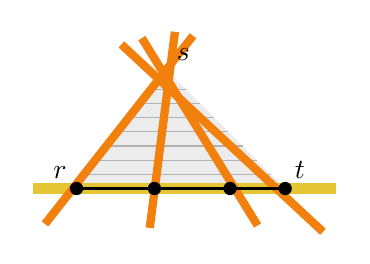
\begin{tikzpicture}[x=1cm,y=1cm]
\fill[gray!15] (0,0)--(1.15,1.5)--(2.65,0)--cycle;
\foreach \y in {.18,.36,.54,.72,.90,1.08,1.26}{\draw[gray!60,thin] ({.7667*\y},\y)--({2.65-\y},\y);}
\draw[yellow!55!brown,line width=4pt] (-.55,0)--(3.3,0);
\draw[orange!80!brown,line width=3pt] (-.4,-.45)--(1.48,1.94);
\draw[orange!80!brown,line width=3pt] (.93,-.5)--(1.25,1.99);
\draw[orange!80!brown,line width=3pt] (2.30,-.47)--(.83,1.91);
\draw[orange!80!brown,line width=3pt] (3.13,-.55)--(.57,1.83);
\draw[thick] (0,0)--(2.65,0);
\foreach \x in {0,.99,1.95,2.65}{\fill (\x,0) circle(2.4pt);}
\node[above right] at (1.15,1.5){$s$};\node[above left] at (0,0){$r$};\node[above right] at (2.65,0){$t$};
\end{tikzpicture}}

\deleted{\unsure{un sous-ens.} de $\nu\geq1$ sur $D$, \deleted{non réduites à un sommet de $\Sigma$, formant} un arc sur $\widetilde D$ (le rev. des \unsure{vis} de $D$, avec sa structure polygonale) et dont les $\nu+1$ sommets s'identifient aux \unsure{$\nu$-arêtes orientations} de $\widetilde D$) \deleted{\unsure{correspondant|correspondent} à $\nu+1$}\inserted{sont \unsure{non-sommets de}} $\Sigma$, et correspondent à des $D_i\in\Sigma$ que se rencontrent en un $=$ point $s$ \uline{d'ordre exactement} $\nu+1$, et sans sommet de $\Sigma$ dans le triangle $s,r,t$ \unsure{ni à l'intérieur, sauf} $s\ldots$}

[On exclut le cas où $\Sigma$ est trivial, qu'il est mieux traiter à part.] On a une application
\diagram{\begin{tikzcd}[ampersand replacement=\&]\widetilde P\arrow[r,"{(\text{source,but})}"]\&P\times P\end{tikzcd}}
qui associe à $(D,T)$ le couple $(D,D')$, où $D'$ est ``déduit de $D$ par balayage-spécialisation de $D$ au dessus de $T$''. Cette application est-elle injective? Quand on connaît $(D,D')$, on connaît aussi $s$ (qui est l'unique sommet de $\Sigma$ qui est dans $D'$, non dans $D$) donc aussi l'ens \deleted{des extrémités} des \inserted{$\nu+1$} sommets de $\Sigma\cup\{D\}$ qui sont inclus dans le triangle $T$ --- savoir les sommets communs à $D$ et aux $\nu+1$ éléments de $\Sigma$ passant par $s$. D'autre part, on voit qu'aucune de ces ps. droites (en tant que p. dr. de \deleted{$\unsure{\Sigma}$} $\Sigma'=\Sigma\cup\{D\}$) n'est un bigone, \deleted{ce qui} (sinon $\Sigma$ serait trivial de centre $s$) ce qui implique que les arêtes \deleted{joignant}\inserted{contenues} dans $T$ qui joignent $s$ aux $2$ sommets \deleted{\unsure{con.}} envisagés sur $D$, \unsure{sont ainsi uniques} \deleted{\unsure{d'autre p.}} \unsure{(les \unsure{vis|vts} de $\Sigma$ que sur $D$!)} \unsure{au moins un autre sommet que ceux-là}, ce qui implique que l'aire qu'ils \unsure{cernent} est également déterminée --- bref, $\widetilde P\to P\times P$ est bien injectif. On trouve donc un \uline{\unsure{graphe}}\inserted{\uline{strict orienté}} \unsure{simple} $P$ comme ens des sommets, $\widetilde P$ comme ens. d'arêtes, ch. que arête étant orientée \deleted{\unsure{d'un sens}}\inserted{(i.e. munie} d'une origine privilégiée).

\margin{\uline{NB} on a tjs $D\ne D'$, car $D'\cap S=(D\cap S)\cup\{s\}$}

Soit, pour $D\in P$, $\operatorname{Sp}_0(D)$ l'ens de ses spécialisations \inserted{(immédiates) ou ``successeurs''}, \deleted{et $\operatorname{Gen}(D)$ l'ens de ses} qui correspond à l'ens des triangles de spécialisation \unsure{formés|\deleted{formés}} pour $D$. Soit de $=$ $\operatorname{Gen}_0(D)$ l'ens de ses générisations (immédiates), qui correspond à l'ens des couples $(s,\widetilde{\unsure{\varphi|\xi}})$, où $s\in D\cap S$, et $\widetilde{\unsure{\varphi|\xi}}$ est une or. de $D$ en $s$ i.e. un pt de $\widetilde D$ sur $s$.

\margin{11}

\scanpage{13}
\mspage{2}

\figure{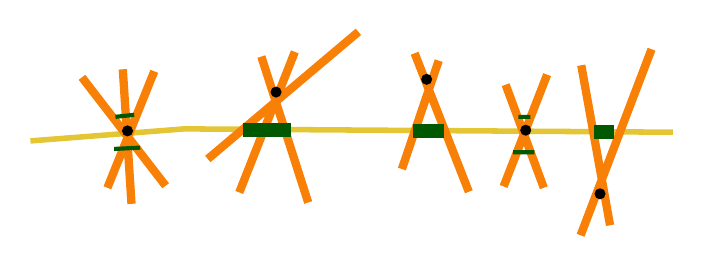
\begin{tikzpicture}[x=.85cm,y=.85cm]
\draw[yellow!55!brown,line width=2pt] (-.6,-.08)--(1.7,.10)--(9,.05);
\draw[orange!90!brown,line width=3pt] (.55,-.78)--(1.25,.96) (.17,.87)--(1.42,-.75) (.78,.99)--(.91,-1.02);
\draw[orange!90!brown,line width=3pt] (2.05,-.35)--(4.3,1.55) (2.52,-.85)--(3.35,1.25) (2.85,1.18)--(3.55,-1.00);
\draw[orange!90!brown,line width=3pt] (4.95,-.50)--(5.50,1.12) (5.14,1.23)--(5.95,-.84);
\draw[orange!90!brown,line width=3pt] (6.47,-.76)--(7.12,.91) (6.5,.76)--(7.07,-.78);
\draw[orange!90!brown,line width=3pt] (7.63,1.05)--(8.06,-1.34) (7.62,-1.49)--(8.68,1.29);
\draw[black!65!green,line width=5pt] (2.57,.08)--(3.29,.08) (5.11,.07)--(5.58,.07) (7.82,.05)--(8.12,.05);
\draw[black!65!green,line width=1.5pt] (.67,.28)--(.95,.31) (.65,-.20)--(1.04,-.18) (6.69,.28)--(6.87,.28) (6.61,-.25)--(6.93,-.25);
\foreach \x/\y in {.85/.07,3.07/.65,5.32/.84,6.80/.08,7.91/-.87}{\fill (\x,\y) circle(2pt);}
\end{tikzpicture}}

Chaque élément de $\operatorname{Sp}_0(D)$ définit un arc \deleted{(fermé)} sur $\widetilde D$, ces arcs étant mutuellement disjoints; chaque pt de $\operatorname{Gen}_0(D)$ définit un \deleted{\unsure{élément}}\inserted{pt} de $\widetilde D$, ces pt étant tous différents et non contenus dans les \deleted{\unsure{alternativement}} arcs précédents. Il en résulte une \uline{structure polygonale} sur l'ens $\operatorname{Sp}_0(D)\amalg\operatorname{Gen}_0(D)$, qui \deleted{\unsure{se}} s'identifie aussi à l'ens des arcs issus du sommet $D$ du graphe $\Gamma(\underline\Sigma)$. \deleted{Ce polygone a au moins}\inserted{Cet ens. a au moins} trois éléments je crois. \deleted{C'est} Il y en a \unsure{en} au moins quatre bien sûr si $\operatorname{card}S\cap D\geq2$, donc il suffit de regarder les cas $\operatorname{card}S\cap D\in\{0,1\}$. Dans le cas d'une $D$ ``stable'' i.e. $\operatorname{card}S\cap D=0$, il faut prouver qu'il y a au moins \deleted{deux} trois triangles de spécialisation, \unsure{disons}, dans le cas \deleted{de} $\operatorname{card}S\cap D=1$ \deleted{il f} (cas sous-stable) il faut montrer qu'il y en a au moins un.

\figure{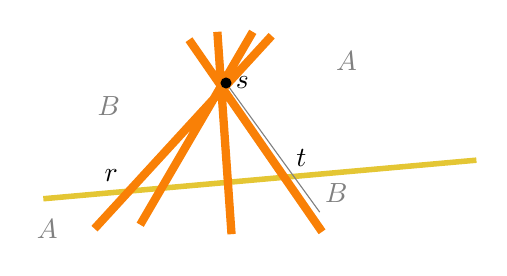
\begin{tikzpicture}[x=1cm,y=1cm]
\draw[yellow!55!brown,line width=2pt] (-.7,.13)--(4.8,.62);
\draw[gray,thin] (.63,-.10)--(1.62,1.6)--(2.81,-.04);
\draw[orange!90!brown,line width=3pt] (-.05,-.25)--(2.20,2.20) (.53,-.20)--(1.96,2.25) (1.69,-.32)--(1.51,2.25) (2.84,-.29)--(1.15,2.15);
\fill (1.62,1.6) circle(2pt);\node[right] at (1.62,1.6){$s$};
\node[above left] at (.37,.23){$r$};\node[above right] at (2.39,.42){$t$};
\node[gray] at (-.65,-.25){$A$};\node[gray] at (.13,1.31){$B$};\node[gray] at (3.15,1.88){$A$};\node[gray] at (3.02,.20){$B$};
\end{tikzpicture}}

a) Cas $D$ stable. On sait que $D$ forme au moins trois triangles (i.e. il y a au moins $3$ triangles de $\Sigma'$ adjacents à $D$), considérons en un. Il est immédiat qu'il est contenu dans un unique triangle de spécialisation $T$. Considérons les deux ``grands triangles'' \deleted{définis} $A$ et $B$ (cf figure) définis par $T$, \deleted{\unsure{adjacents}} adjacents le long de l'arc extérieur $(t,r)$ sur $D$, et \deleted{\unsure{ayant comme côtés}}\inserted{incidents resp. à $(s,r)$ et à $(s,t)$}. Dans chacun, il y a un triangle au moins de $\unsure{\widetilde\Sigma|\Sigma'}$, adjacent à $D$. Chacun de ces triangles est contenu à son tour dans un unique triangle de spécialisation, $T'$ resp. $T''$. D'où les trois triangles cherchés $T,T',T''$.

b) Cas $D$ sous-stable. \inserted{Soit $a$ le sommet de $\Sigma$ qui est \unsure{sur $D$}.} Il y a au moins \uline{trois} triangles \deleted{de} de $\Sigma'$ adj. à $D$, \deleted{\unsure{pour montrer}} \deleted{\unsure{on doit les considérer}}\inserted{Considérons une générisation $D'$ de $D$}, sur laquelle on ``éclate'' un arc $bc$ (cf. figure), \unsure{l'un|pour} des triangles de

\margin{12}

\scanpage{14}
\mspage{3}

\figure{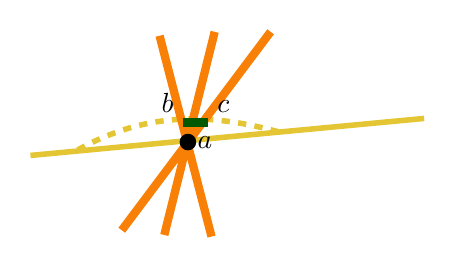
\begin{tikzpicture}[x=1cm,y=1cm]
\draw[yellow!55!brown,line width=2pt] (-2,-.17)--(3,.30);
\draw[yellow!55!brown,line width=2pt,dashed] (-1.4,-.1) .. controls(-.5,.40) and (.3,.36).. (1.15,.13);
\draw[orange!90!brown,line width=3pt] (-.36,1.35)--(.30,-1.2) (.34,1.40)--(-.30,-1.18) (1.05,1.40)--(-.84,-1.12);
\draw[black!65!green,line width=3pt] (-.06,.25)--(.25,.25);
\fill (0,0) circle(3pt);\node[right] at (0,0){$a$};\node[above left] at (-.06,.25){$b$};\node[above right] at (.25,.25){$c$};
\end{tikzpicture}}

spécialisation $(abc)$ de $D'$. Il y a au moins deux autres triangles de spécialisation pour $D'$, qui auront une base sur $D'$ \deleted{qui} qui rencontre $(b,c)$ au plus en un sommet. Si l'un d'eux ne contient ni $b$ ni $c$, on a gagné. Sinon, on a la figure

\margin{\deleted{\unsure{mais?}} \deleted{\unsure{fausse!}}}

\figure{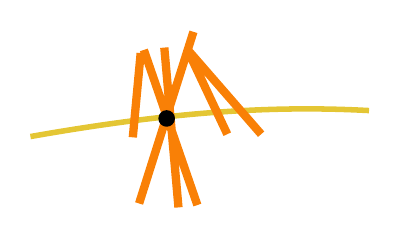
\begin{tikzpicture}[x=1cm,y=1cm]
\draw[yellow!55!brown,line width=2pt] (-1.7,-.15) .. controls(0,.15) and (1.3,.25)..(2.6,.18);
\draw[orange!90!brown,line width=3pt] (-.26,.95)--(.42,-1.02) (0,.98)--(.18,-1.05) (.37,1.18)--(-.32,-1.00) (-.30,.91)--(-.40,-.16) (.29,.96)--(.80,-.12) (.29,.96)--(1.23,-.12);
\fill (.03,.08) circle(3pt);
\end{tikzpicture}}

\figure{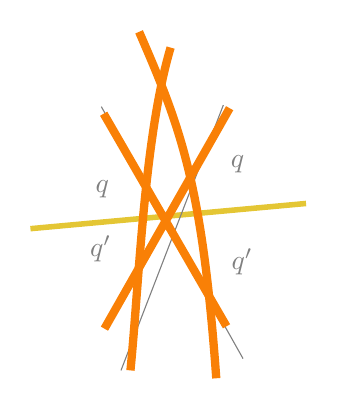
\begin{tikzpicture}[x=1cm,y=1cm]
\draw[yellow!55!brown,line width=2pt] (-1.8,-.10)--(1.7,.22);
\draw[gray,thin] (-.9,1.45)--(.9,-1.75) (.65,1.47)--(-.65,-1.9);
\draw[orange!90!brown,line width=3pt] (-.42,2.40) .. controls(.10,1.20) and (.38,.50)..(.56,-2.0);
\draw[orange!90!brown,line width=3pt] (-.02,2.20) .. controls(-.36,1.05) and (-.42,-.8)..(-.53,-1.9);
\draw[orange!90!brown,line width=3pt] (-.87,1.36)--(.69,-1.34) (.73,1.43)--(-.86,-1.37);
\node[gray,left] at (-.68,.40){$\unsure{q}$};\node[gray,right] at (.62,.72){$\unsure{q}$};\node[gray,left] at (-.65,-.35){$\unsure{q'}$};\node[gray,right] at (.63,-.52){$\unsure{q'}$};
\end{tikzpicture}}

Il y a effectivement un contre-exemple avec $\Sigma=\unsure{\mathrm{St}_4}$, et $D$ \deleted{\unsure{dans}} la position sous-stable qui évite les deux couloirs incidents à $a$, et coupe longitudinalement le troisième.

Mais je m'aperçois que dans la description de l'ens des sommets $P=\operatorname{PR}(\Sigma)$ de $\Gamma$, j'ai oublié les cas les plus importants --- les p.r. \uline{supercritiques}, correspondant aux droites de $\Sigma$ lui-$=$! Il faut que je décrive alors quelles sont les spécialisations vers un tel $\Delta$. Il est clair qu'elles \unsure{ne doit|ne dvt} se faire à \uline{partir d'une position stable} \inserted{(car ce sont des spécialisations \uline{immédiates},)} au contraire --- on doit avoir $\operatorname{Card}(S\cap D)=1$ i.e. $D$ sous-stable. Soit $S\cap D=\{a\}$, il faut que $a$ soit un sommet de $\Delta$, d'autre part, il doit y avoir un secteur biangulaire global dans $X$, défini par $D,\Delta$, qui soit un ``\uline{couloir}'' et la spécialisation se fait en suivant ce couloir, qu'on pourrait nommer \uline{couloir de spécialisation}.

\figure{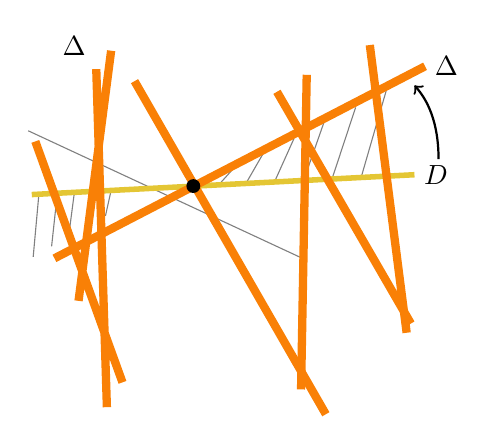
\begin{tikzpicture}[x=.9cm,y=.9cm]
\draw[gray,thin] (-2.45,.80)--(1.42,-1.0);
\draw[gray,thin] (-2.3,-.1)--(-2.38,-.98) (-2.04,-.09)--(-2.12,-.83) (-1.80,-.08)--(-1.88,-.69) (-1.55,-.06)--(-1.63,-.53) (-1.28,-.04)--(-1.36,-.40);
\draw[gray,thin] (.25,.05)--(.43,.25) (.63,.07)--(.86,.47) (1.03,.09)--(1.30,.69) (1.44,.11)--(1.72,.91) (1.84,.13)--(2.17,1.13) (2.25,.15)--(2.60,1.36);
\draw[yellow!55!brown,line width=2pt] (-2.4,-.1)--(3.0,.18);
\draw[orange!90!brown,line width=3pt] (-2.08,-1.00)--(3.15,1.71);
\draw[orange!90!brown,line width=3pt] (-2.35,.65)--(-1.12,-2.75) (-1.28,1.93)--(-1.74,-1.60) (-1.49,1.67)--(-1.34,-3.10) (-.95,1.50)--(1.75,-3.2);
\draw[orange!90!brown,line width=3pt] (1.06,1.35)--(2.95,-1.92) (1.48,1.59)--(1.40,-2.85) (2.37,2.01)--(2.89,-2.05);
\fill (-.12,.02) circle(2.5pt);
\node[above left] at (-1.5,1.72){$\Delta$};\node[right] at (3.15,1.71){$\Delta$};\node[right] at (3,.18){$D$};
\draw[->,thick] (3.34,.40) .. controls(3.34,.93) and (3.18,1.24)..(3.00,1.44);
\end{tikzpicture}}

Il peut y avoir aussi un couloir de spécialisation, sur chaque \unsure{vis} de $D\setminus\{a\}$. Quoi qu'il en soit, on considérera les couloirs de spécialisation \inserted{pour $D$} comme ``équivalents'' à un triangle de sp. pour $D$.

\margin{13}

\scanpage{15}
\mspage{4}

Quand il y en a un, l'autre vis de $D\setminus\{\unsure{a|s}\}$ reste libre pour \deleted{\unsure{encore}} être base de triangles de spécialisation pour $D$ (il y en a deux sur la figure ci-dessus). L'ennui, c'est que les \deleted{\unsure{arcs de}}\inserted{\unsure{ou les couloirs de}} spécialisation ne forment pas, avec les autres spéc. et gén. immédiates une structure polygonale \inserted{naturelle}. \deleted{Mais}
\margin{\unsure{mais?} cf plus bas}
\deleted{si $D$ est orienté ou pas}

Peut-être est-il plus instructif de partir de $\Delta$, et regarder l'ens. de ce qu'il convient d'appeler les ``générisations'' \inserted{(immédiates)}. J'en vois de deux

\figure{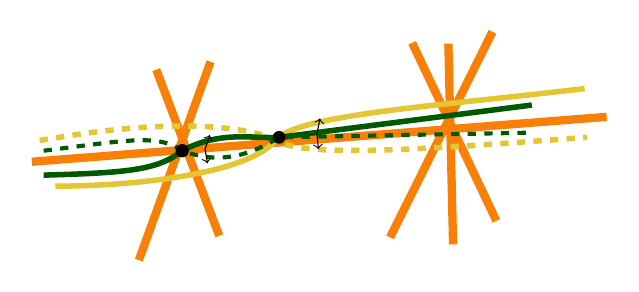
\begin{tikzpicture}[x=1cm,y=1cm]
\draw[orange!90!brown,line width=3pt] (-2.6,-.17)--(4.7,.40);
\draw[orange!90!brown,line width=3pt] (-1.02,1.00)--(-.22,-1.11) (-.33,1.10)--(-1.24,-1.42);
\draw[orange!90!brown,line width=3pt] (2.23,1.34)--(3.30,-.92) (2.69,1.33)--(2.75,-1.22) (3.25,1.48)--(1.95,-1.13);
\draw[yellow!55!brown,line width=2pt] (-2.30,-.48) .. controls(-1.2,-.48) and(.2,-.30)..(.50,.11) .. controls(.80,.43) and (2.5,.53)..(4.42,.76);
\draw[yellow!55!brown,line width=2pt,dashed] (-2.5,.10) .. controls(-.8,.40) and(.1,.28)..(.50,.11) .. controls(.8,-.15) and(2.8,.02)..(4.45,.14);
\draw[green!35!black,line width=2pt] (-2.45,-.34) .. controls(-1.4,-.31) and(-1.0,-.28)..(-.69,-.03) .. controls(-.2,.23) and(.2,.12)..(.54,.14) --(3.75,.55);
\draw[green!35!black,line width=1.5pt,dashed] (-2.45,-.03) .. controls(-1.4,.10) and(-1.0,.19)..(-.69,-.03) .. controls(-.2,-.22) and(.2,-.07)..(.54,.14)--(3.77,.20);
\fill (-.69,-.03) circle(2.4pt);\fill (.54,.14) circle(2.3pt);
\draw[->,thin] (-.40,-.01)--(-.34,.17);\draw[->,thin] (-.40,-.01)--(-.37,-.19);
\draw[->,thin] (1.02,.18)--(1.06,.38);\draw[->,thin] (1.02,.18)--(1.04,-.01);
\end{tikzpicture}}

types, \uline{les stables}, \deleted{et les sous-stables}. Pour les stables, j'en vois deux pour chaque côté, correspondant aux $2$ orientations superficielles le long de l'arête.

\margin{les stables ne sont pas des gén. \uline{immédiates} pourtant, \unsure{ces gén. se} \uline{factorisent} par les sous stables}

Pour les sous-stables, j'en vois également deux pour chaque sommet, correspondant aux deux orientations de $X$ en ce sommet. Ainsi l'ens des \deleted{\unsure{vis}} générisations correspond à l'ens des sommets et des arêtes \unsure{de ce vrai} polygône topologique, image inverse de $\Delta$ dans $\widetilde X$. On fera attention que ce polygône n'est \unsure{\uline{pas}|\deleted{pas}} canoniquement isom. au polygône des vis qu'on avait regardé pour les p.r. $D$ non supercritiques --- le choix d'un isom. dépend du choix d'une orientation de $\Delta$. Tjrs est-il que si $\nu$ est le nb de sommets de $\Delta$, l'ens des générisations \inserted{immédiates} de $\Delta$ s'identifie aux sommets d'un \deleted{\unsure{ens.}} polygône \unsure{croisé} d'ordre \uline{$2\nu+2\nu=4\nu$}$^*$, rev. d'ordre $2$ du collier défini par $\Delta$. L'une des orientations de ce polygône est liée donc à l'une des orientations de $\Delta$ lui-$=$.

\margin{$^*$ ou, d'ordre $2\nu$ seulement en se bornant aux gén. \uline{immédiates}}
\margin{14}

\scanpage{16}
\mspage{5}

\figure{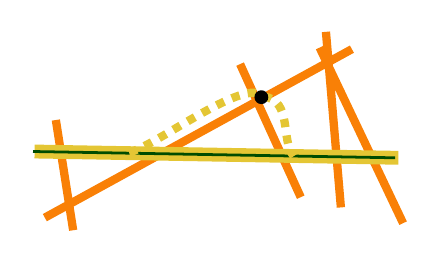
\begin{tikzpicture}[x=1cm,y=1cm]
\draw[orange!90!brown,line width=3pt] (-2.1,-.74)--(1.8,1.40) (-1.96,.50)--(-1.74,-.90) (.38,1.21)--(1.15,-.48) (1.39,1.42)--(2.45,-.81) (1.47,1.62)--(1.66,-.61);
\draw[yellow!55!brown,line width=5pt] (-2.23,.10)--(2.39,.02);
\draw[green!30!black,line width=1pt] (-2.25,.10)--(2.35,.02);
\draw[yellow!55!brown,line width=3pt,dashed] (-1.03,.09) .. controls(-.7,.16) and(.45,1.06)..(.68,.80) .. controls(1.05,.74) and (.89,.25)..(1.06,.04);
\fill (.65,.79) circle(2.5pt);
\end{tikzpicture}}

Revenant à une p.r. $D$ sous-stable passant par $a\in S$, on peut considérer que \deleted{\unsure{les}} (si $\widetilde D$ désigne le rev. des vis) un couloir de spécialisation correspond à un \uline{arc ouvert} de $\widetilde D$, d'extrémités les deux sommets $a',a''$ de $\widetilde D$ au-dessus de $a$. \deleted{En identifiant} \deleted{De façon} Ainsi on peut dire que \deleted{les générisations et} spécialisations de $D$ sont données par des arcs ouverts de $\widetilde D\setminus\{a',a''\}$, mutuellement disjoints, donc contenus dans l'une ou l'autre comp. conn. $\widetilde D_1,\widetilde D_2$ de $\widetilde D\setminus\{a',a''\}$. \deleted{Il y en a}\inserted{Ainsi}, on voit qu'elles forment une \unsure{structuration polygonale des arcs} ``$a',a''$'', et comme sur $\widetilde D_1,\widetilde D_2$ il y a au moins un arc de spécialisation, on voit que le nb total de sommets du polygône de spécialisation-générisation est au moins égal à quatre. \deleted{\unsure{C'est}}

\uline{Ainsi} Dans le graphe \inserted{strict orienté} $\Gamma(\underline\Sigma)$ (où on n'oubliera pas comme sommets les p.r. supercritiques), \deleted{\unsure{chacun des arêtes}}\inserted{pour tt sommet $D$}, l'ens des \deleted{arêtes} arcs qui en sortent $(\simeq\operatorname{Spec}_0(D)\amalg\operatorname{Gen}_0(D))$ est de cardinal au moins $3$ (et au moins $4$ si $D$ n'est pas stable \inserted{i.e. admet une générisation}). Il est muni d'une structure polygonale \inserted{naturelle}, dont l'ens des orientations est \inserted{can. isom. à} l'ens des orientations de $D$. Pour tt flè. de spécialisation \inserted{$D\longrightarrow D'$}, on trouve une iso. can. entre $\omega(D)$ et $\omega(D')$.

[NB L'ens des générisations \inserted{$\operatorname{Gen}_0(D)$} \inserted{de $D$} s'identifie à l'image \deleted{des} inverse de $D\cap S$ dans $\widetilde D$, où pour $D$ non supercritique, $\widetilde D$ désigne le rev. des vis, et pour $D$ supercritique, le rev. image inverse dans $\widetilde X$. Toute flèche

\margin{15}

\scanpage{17}
\mspage{6}

de spécialisation $D\mathbin{-}D'$ définit une flèche $\operatorname{Gen}_0(D)\hookrightarrow\operatorname{Gen}_0(D')$ injective, dont le complémentaire est formé de deux \deleted{sommets} éléments \deleted{$\unsure{a}$}.

\deleted{\unsure{Immersion}}\inserted{Plongement} cellulaire canonique de $\Gamma(\underline\Sigma)$ dans une surface \deleted{\unsure{combinatoire}}\inserted{$\operatorname{Str}(\underline\Sigma)$ (la surface structurale)}

Sommets stables: toutes les arêtes qui en sortent \uline{partent} de $D$
\figure{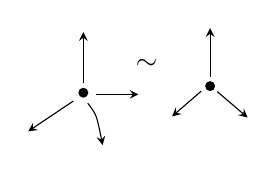
\begin{tikzpicture}[x=.7cm,y=.7cm,>=stealth]
\fill (0,0) circle(1.8pt);\draw[->] (0,.18)--(0,1.1);\draw[->] (-.18,-.15)--(-1,-.70);\draw[->] (.08,-.19)..controls(.24,-.4)..(.35,-.95);\draw[->] (.23,-.03)--(1,-.03);
\node at (1.15,.52){$\sim$};
\fill (2.3,.12) circle(1.8pt);\draw[->] (2.3,.28)--(2.3,1.17);\draw[->] (2.14,.03)--(1.61,-.43);\draw[->] (2.43,.02)--(2.98,-.45);
\end{tikzpicture}}

Sommets sous-stables: il y a exactt \uline{deux} arêtes qui \uline{arrivent} à $D$
\figure{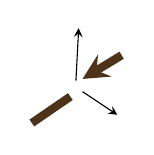
\begin{tikzpicture}[x=.7cm,y=.7cm,>=stealth]
\draw[->] (0,.17)--(.05,1.12);\draw[->] (.12,-.03)--(.75,-.45);
\draw[->,brown!40!black,line width=3pt] (-.8,-.60)--(-.1,-.12) (.83,.63)--(.12,.20);
\end{tikzpicture}}

Sommets critiques: au moins quatre arêtes qui arrivent à $D$
\figure{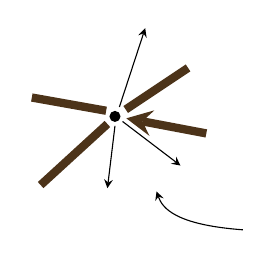
\begin{tikzpicture}[x=.8cm,y=.8cm,>=stealth]
\fill (0,0) circle(2pt);\draw[->] (.07,.15)--(.48,1.4);\draw[->] (0,-.15)--(-.12,-1.14);\draw[->] (.12,-.08)--(1.04,-.78);
\draw[->,brown!40!black,line width=3pt] (-1.32,.30)--(-.14,.09) (-1.18,-1.09)--(-.12,-.12) (1.16,.77)--(.17,.11) (1.45,-.27)--(.18,-.03);
\draw[->] (2.03,-1.80).. controls(.95,-1.72) and (.75,-1.45)..(.66,-1.19);
\end{tikzpicture}}

Sommets critiques \deleted{\unsure{et}} extrémaux: toutes les arêtes en $D$ \uline{arrivent} à $D$
\figure{
\begin{tikzpicture}[x=.7cm,y=.7cm,>=stealth]
\fill (0,0) circle(2pt);\draw[->,brown!40!black,line width=3pt] (-.85,.85)--(-.12,.11) (.77,.86)--(.11,.12) (-.81,-.92)--(-.10,-.12) (.81,-.88)--(.12,-.13);
\end{tikzpicture}}

\uline{Toute arête} de $\Gamma(\underline\Sigma)$ est munie d'un \uline{poids} $(\in\mathbf N^*)$ qui \inserted{est le} \deleted{\unsure{pour une arête de spécialisation}} \deleted{\unsure{également exprimé}} \inserted{\unsure{nb d'arêtes}} \deleted{de} $D$ (ou resp. de $\Sigma'$, interceptées par l'arc de spécialisation) --- dans le cas de la figure ci-contre, correspondant au triangle de spécialisation $T$.

\figure{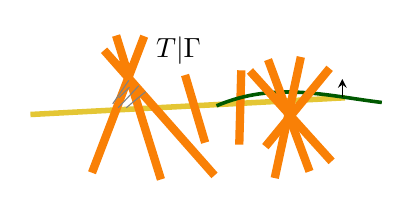
\begin{tikzpicture}[x=.85cm,y=.85cm,>=stealth]
\draw[yellow!55!brown,line width=2pt] (-1.6,-.05)--(3.1,.20);
\draw[orange!90!brown,line width=3pt] (-.68,-.92)--(.1,1.12) (-.32,1.13)--(.35,-1.02) (-.50,.91)--(1.15,-.96) (.71,.54)--(1.01,-.47) (1.55,.61)--(1.52,-.50);
\draw[gray,thin] (-.28,.20)--(-.12,.36) (-.37,.11)--(-.13,.46) (-.29,.05)--(.02,.38) (-.17,.05)--(.12,.29);
\node[above right] at (.13,.55){$\unsure{T|\Gamma}$};
\draw[green!35!black,line width=1.3pt] (1.18,.08)..controls(2.05,.45) and (2.82,.23)..(3.65,.13);
\foreach \a/\b/\c/\d in {1.68/.60/2.90/-.75,1.95/.77/2.57/-.90,2.44/.81/2.05/-1.0,2.87/.64/1.91/-.53}{\draw[orange!90!brown,line width=3pt](\a,\b)--(\c,\d);}
\draw[->] (3.06,.21)--(3.06,.48);
\end{tikzpicture}}

Tout secteur cellulaire local de $\operatorname{Str}(\underline\Sigma)$ en un sommet $D$ correspond à un arc de $\widetilde D$, \deleted{correspondant à l'arc}\inserted{simple} \uline{l'arc} compris entre deux arcs de spécialisation consécutifs, ou deux \deleted{arcs de} sommets de \deleted{spécialisation}\inserted{générisation} consécutifs (sur $\widetilde D$, sans aucun arc de spécialisation entre), ou les cas mixtes; le nb d'arêtes sur cet arc (au sens de $\Sigma'$) est appelé encore \uline{poids} du secteur angulaire. Avec ces données, on trouve une \uline{carte cellulaire} \deleted{pondérée} \uline{à graphe orienté}, et à arêtes et ``coins'' \uline{pondérés}. On a d'autre part, pour tt sommet $D$,

\margin{\deleted{\unsure{de toutes les}} somme des \inserted{pondérations de} toutes les arêtes en $D$, et des \inserted{pondérations de} tous les coins en $D$ \deleted{$\unsure{\longleftarrow}$} est égale à $2n$ (où $n=\operatorname{card}\Sigma$)}
\margin{16}

\scanpage{18}
\mspage{7}
\margin{17}

Plus précisément, considérons le polygône combinatoire déduit du polygône combinatoire $\operatorname{Pol}(D)$ de $D$ sur $\operatorname{Str}(\underline\Sigma)$, en ``éclatant'' chaque sommet (correspondant à une arête de $\Gamma(\underline\Sigma)$ en $D$) en autant de sommets que l'indique son poids, et en plaçant sur chaque arête (correspondant à un coin de $\operatorname{Str}$ en $D$) autant de pts que l'indique son poids. On trouve un polygône $\widehat{\operatorname{Pol}}(D)$, \deleted{\unsure{Ceci dit,}} dont les sommets correspondent aux arêtes découpées sur \deleted{$\unsure{D}$} $\widetilde D$, visualisé comme un contour parallèle à $D$, \inserted{par les $\Delta_i$ ($\Sigma$);} (donc ses \uline{arêtes} correspondent aux sommets découpés par les $\Delta_i$ sur $\widetilde D$ --- \deleted{\unsure{de}} par $\Delta_i$ \deleted{\unsure{les éléments}} Si $I$ est l'ens d'indices pour $\Sigma$, $\widetilde I$ l'ens d'indices pour l'ens des $\vec\Delta_i$ orientés, on trouve donc une correspondance biunivoque can.
\[
\widetilde I\simeq\text{ens des arêtes de }\widehat P(D)
\]
d'où la relation \deleted{\unsure{de}} numérique plus haut. \deleted{\unsure{Cette}} Comme $\widehat P(D)$ est donc d'ordre $2n$, il admet une antipodie, $\widetilde I$ aussi --- et la bijection est compatible avec les antipodies.

\margin{\uline{NB} Le $\unsure{\widetilde{\widehat P}(D)|\widehat{\widehat P}(D)}$ défini \unsure{comme l'ens} des sommets de $\widehat P(D)$ qui étaient ``\unsure{au dessus}'' de sommets de $P(D)$, est stable pour l'antipodie.}

\deleted{\unsure{Ainsi} \illegible{2}} \unsure{À présent} examinons à part le cas de $D$ supercritique, soit \deleted{$\unsure{D}$}
\[
D\equiv\Delta=\Delta_{i_0},
\]
auquel cas il n'y a \deleted{\unsure{pas}} que des arêtes de généristé, issues de $D_j\to\Delta$, qui correspondent aux \deleted{\unsure{éléments}} \inserted{pts} de $\widetilde\Delta$ ($={}$ image inv. de $\Delta$ dans $\widetilde X$) qui sont au dessus des sommets sur $\Delta$.

\figure{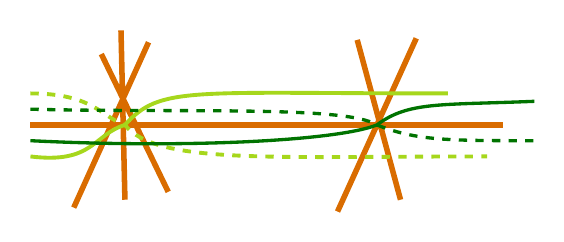
\begin{tikzpicture}[x=1cm,y=1cm]
\draw[orange!85!black,line width=2pt] (0,0)--(6,0);
\draw[orange!85!black,line width=2pt] (.55,-1.05)--(1.5,1.05) (1.2,-.95)--(1.15,1.2) (1.75,-.85)--(.9,.9);
\draw[orange!85!black,line width=2pt] (3.9,-1.1)--(4.9,1.1) (4.7,-.95)--(4.15,1.08);
\draw[yellow!65!green,line width=1.4pt] (0,-.4)..controls(.8,-.5)and(.8,-.12)..(1.2,0)..controls(1.65,.5)and(2,.4)..(5.3,.4);
\draw[yellow!65!green,line width=1.4pt,dashed] (0,.4)..controls(.8,.4)and(.9,.1)..(1.2,0)..controls(1.6,-.5)and(3,-.4)..(5.8,-.4);
\draw[green!45!black,line width=1.2pt] (0,-.2)..controls(2,-.3)and(3.9,-.2)..(4.4,0)..controls(4.8,.3)and(5.2,.25)..(6.4,.3);
\draw[green!45!black,line width=1.2pt,dashed] (0,.2)..controls(2,.15)and(4,.25)..(4.4,0)..controls(4.9,-.2)and(5.3,-.2)..(6.4,-.2);
\end{tikzpicture}}

\unsure{Choisissons} une orientation de $\Delta$, qui permet d'identifier $\widetilde\Delta$ en une des vis de $\Delta$. Nous affectons chaque arête \inserted{de $\Gamma(\underline\Sigma)$} issue de $\Delta$, \unsure{correspondante|correspondant} à \unsure{une généristé} $s\in S\cap\Delta$, des ``poids'' (\unsure{modifiés p.r.} à la définition précédente) égal au \deleted{\unsure{distinctes de $\Delta$},} \inserted{Nb.} des pdroites ($\Sigma_i$ \deleted{\unsure{qui sont}} \deleted{$\unsure{\Delta}$} \uline{distinctes de $\Delta$} qui passent en $s$, i.e. le nb de \uline{sommets} découpés au voisinage de $s$ par une ``parallèle'' (un côté) à $\Delta$.

\figure{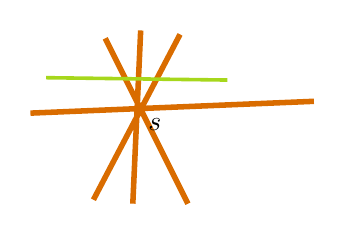
\begin{tikzpicture}[x=1cm,y=1cm]
\draw[orange!85!black,line width=2pt] (-1.4,0)--(2.2,.15) (-.6,-1.1)--(.5,1) (-.1,-1.15)--(0,1.05) (.6,-1.15)--(-.45,.95);
\draw[yellow!65!green,line width=1.3pt] (-1.2,.45)--(1.1,.42);
\node at (.18,-.15) {$s$};
\end{tikzpicture}}

Si nous ``éclatons'' chaque arête de $\Gamma(\underline\Sigma)$, en autant de sommets de

\scanpage{19}
\mspage{8}
\margin{18}

$\operatorname{Pol}(D)$, en autant de sommets que l'indique son poids, on trouve un nouveau polygône combinatoire \inserted{$\widehat P(\Delta)$}, d'ordre $2(n-1)$, semblable à celui découpé par les $\Delta_i$ ($i\ne i_0$) sur une \uline{parallèle} à $\Delta$. Et on trouve une bijection canonique
\[
\widetilde{I\setminus\{i_0\}}\simeq\text{ens des \uline{sommets} de }\widehat P(\Delta_{i_0})
\]
compatible avec les antipodies.

\margin{NB Cette bijection dépend du choix d'une orientation de $\Delta_{i_0}$ --- en le changeant, on trouve la précédente composée avec l'antipodisme.}

\deleted{\figure{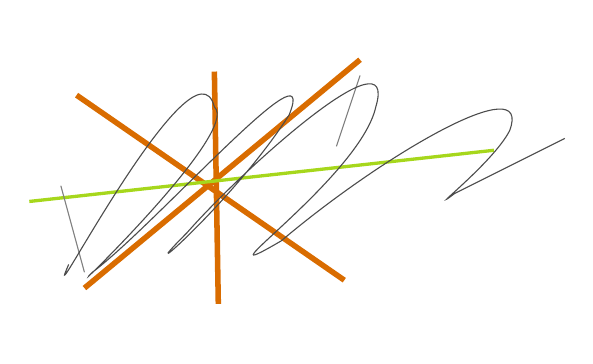
\begin{tikzpicture}[x=1cm,y=1cm]
\draw[orange!85!black,line width=2pt] (-1.7,-1.3)--(1.8,1.6) (-1.8,1.15)--(1.6,-1.2) (0,-1.5)--(-.05,1.45);
\draw[yellow!65!green,line width=1.2pt] (-2.4,-.2)--(3.5,.45);
\draw[gray,thin] (-1.7,-1.1)--(-2,0) (1.5,.5)--(1.8,1.4);
\draw[black!70] (-1.9,-1)..controls(-2.3,-1.9)and(-.3,2)..(-.05,1)..controls(.3,.7)and(-2,-1.5)..(-1.6,-1.1)..controls(-.8,-.5)and(1.3,1.9)..(.9,.9)..controls(.2,-.2)and(-1.2,-1.4)..(-.4,-.6)..controls(.3,.2)and(2.3,2)..(2,1)..controls(1.8,.1)and(-.4,-1.4)..(.8,-.7)..controls(2.1,.4)and(4,1.5)..(3.7,.7)..controls(3.5,.3)and(2.6,-.4)..(3,-.1)--(4.4,.6);
\end{tikzpicture}}}

\figure{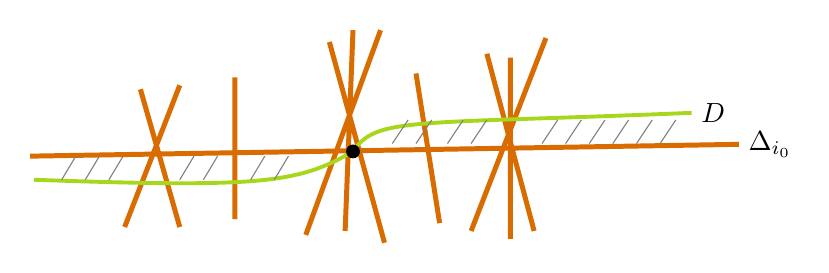
\begin{tikzpicture}[x=1cm,y=1cm]
\draw[orange!85!black,line width=1.8pt] (0,0)--(9,.15);
\draw[orange!85!black,line width=1.8pt] (1.2,-.9)--(1.9,.9) (1.9,-.9)--(1.4,.85) (2.6,-.8)--(2.6,1) (3.5,-1)--(4.45,1.6) (4,-.95)--(4.1,1.6) (4.5,-1.1)--(3.8,1.45) (5.2,-.85)--(4.9,1.05) (6.1,-1.05)--(6.1,1.25) (5.6,-.95)--(6.55,1.5) (6.4,-.95)--(5.8,1.3);
\draw[yellow!65!green,line width=1.4pt] (.05,-.3)..controls(2.9,-.4)and(3.4,-.35)..(4.1,.06)..controls(4.4,.5)and(4.8,.4)..(8.4,.55);
\foreach \x in {.4,.7,1,1.9,2.2,2.8,3.1}{\draw[gray,thin] (\x,-.3)--+( .18,.3);}
\foreach \x in {4.6,4.9,5.3,5.6,6.5,6.8,7.1,7.4,7.7,8}{\draw[gray,thin] (\x,.16)--+(.2,.3);}
\fill (4.1,.06) circle (2.5pt);
\node[right] at (8.4,.55) {$D$};\node[right] at (9,.15) {$\Delta_{i_0}$};
\end{tikzpicture}}

On aimerait comparer la pondération modifiée d'une arête en $\Delta$, avec sa pondération ordinaire. On trouve pour la pondération ordinaire $\nu_0$
\[
\begin{aligned}
\nu_0&=\text{Nb d'arêtes découpées sur la \unsure{ligne} $\unsure{D|\Delta}$ par $\Sigma$ le long}\\
&\qquad\text{du couloir}=\text{nb d'arêtes en }D=\deleted{\unsure{\operatorname{Card}(S\cap D)}}\ n-\nu.
\end{aligned}
\]
donc
\[
\nu+\nu_0=n
\]
donc la pondération modifiée résulte de la pondération ordinaire (si on connaît $n$. --- mais $n$ est déduit de la pondération ordinaire par les formules locales $\sum\text{de toutes les pondérations en }D=2n$ (où $D$ est un sommet non supercritique, p.ex. stable).

\deleted{\unsure{A}} On a ainsi trouvé une application canonique
\diagram{\begin{tikzcd}[ampersand replacement=\&,column sep=large]
\underbrace{\text{Sommets de }\Gamma(\underline\Sigma)}_{(=\operatorname{Pr}(\underline\Sigma))}\setminus\underbrace{\Sigma}_{\substack{\text{p.r. super}\\\text{critiques}}} \arrow[r] \& \substack{\text{ens des structures}\\\text{polygonales sur }\widetilde I\\\text{compatibles avec l'antipodisme,}}
\end{tikzcd}}
et il ne devrait pas être difficile de montrer que cette application est \uline{injective}. Il faudrait de plus, pour bien faire, voir :

1) Comment ``varient'' les $P(\unsure{D|\Delta})$, $\widehat P(\unsure{D|\Delta})$ le long d'une flèche de spécialisation,

\scanpage{20}
\mspage{9}
\margin{19}

et

2°) Comment interpréter toute la structure de graphe orienté à plongement cellulaire, avec pondérations des arêtes et des coins, en termes de l'interprétation de ses sommets \deleted{\unsure{en termes}} \inserted{comme} des str. polygonales sur $\widetilde I$.

\deleted{\unsure{Pour}}

\figure{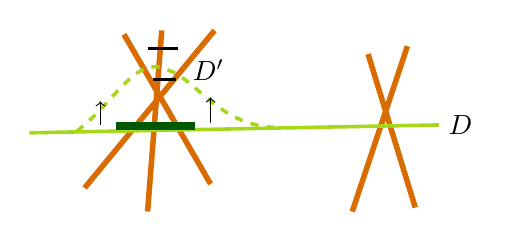
\begin{tikzpicture}[x=1cm,y=1cm]
\draw[orange!85!black,line width=2pt] (-.8,-.7)--(.85,1.3) (.8,-.65)--(-.3,1.25) (0,-1)--(.18,1.3) (2.6,-1)--(3.3,1.1) (3.4,-.95)--(2.8,1);
\draw[yellow!65!green,line width=1.3pt] (-1.5,0)--(3.7,.1);
\draw[yellow!65!green,line width=1.3pt,dashed] (-.9,.02)..controls(-.4,.4)and(-.15,1)..(.25,.8)..controls(.6,.7)and(.9,.1)..(1.6,.07);
\draw[green!35!black,line width=3pt] (-.4,.09)--(.6,.09);
\draw[black,line width=1.2pt] (.07,.68)--(.36,.68) (.01,1.07)--(.38,1.07);
\draw[->] (-.6,.1)--(-.6,.4);\draw[->] (.8,.12)--(.8,.45);
\node[right] at (3.7,.1) {$D$};\node[right] at (.45,.8) {$D'$};
\end{tikzpicture}}

Pour 1°) L'examen de la situation \inserted{($D\to D'$ dans le cas ``ordinaire'' ($D'$ non supercritique))} montre que $\unsure{\widehat{\operatorname{Pol}}(D)}$ et $\unsure{\widehat{\operatorname{Pol}}(D')}$, i.e. l'ens des arêtes sur $\widetilde{\widetilde D}$ et sur $\widetilde{\widetilde D'}$ (où le $\approx$ indique la ``parallèle'') \inserted{i.e. des demi-arêtes en $D$ et en $D'$} sont les ``$=$'', \deleted{\unsure{et}} \uline{sauf} \deleted{sur les} au voisinage des deux paquets de points antipodiques, correspondant \deleted{aux} en $D$ à \inserted{l'éclatement de} l'arête de spécialisation issue de $D$ (\unsure{et sur l'antipodique}), et en $D'$ l'inverse. De façon plus précise,

\figure{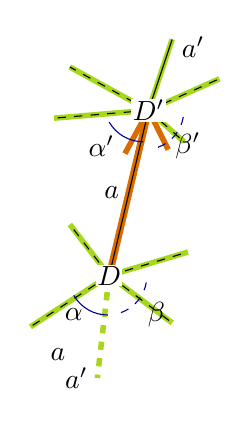
\begin{tikzpicture}[x=1cm,y=1cm]
\coordinate (D) at (0,0);\coordinate (E) at (.5,2.1);
\draw[orange!85!black,line width=2.5pt] (D)--(E);
\draw[->,black] (D)--(E) node[midway,left] {$a$};
\foreach \p in {(-1,-.65),(-.5,.65),(.8,-.6),(1,.3)}{\draw[yellow!65!green,line width=2pt] (D)--\p;\draw[dashed] (D)--\p;}
\draw[yellow!65!green,line width=2pt,dashed] (0,0)--(-.15,-1.3);\node[left] at(-.15,-1.3){$a'$};
\foreach \p in {(-.5,2.65),(-.7,2),(.95,1.7),(1.4,2.5)}{\draw[yellow!65!green,line width=2pt] (E)--\p;\draw[dashed] (E)--\p;}
\draw[yellow!65!green,line width=2pt] (E)--(.8,3);\draw[->] (.8,3)--(E);\node[right]at(.8,2.9){$a'$};
\draw[orange!85!black,line width=2pt] (E)--(.2,1.55) (E)--(.75,1.6);
\draw[blue!60!black] (-.45,-.25) arc[start angle=210,end angle=270,radius=.5];\node at(-.45,-.5){$\alpha$};
\draw[blue!60!black,dashed] (.15,-.47) arc[start angle=290,end angle=350,radius=.5];\node at(.6,-.5){$\beta$};
\draw[blue!60!black] (0,1.95) arc[start angle=210,end angle=270,radius=.5];\node at(-.1,1.65){$\alpha'$};
\draw[blue!60!black,dashed] (.62,1.63) arc[start angle=290,end angle=350,radius=.5];\node at(1,1.65){$\beta'$};
\node[fill=white,inner sep=.5pt] at(D){$D$};\node[fill=white,inner sep=.5pt]at(E){$D'$};
\node at(-.65,-1){$\deleted{\unsure{a}}$};
\end{tikzpicture}}

\figure{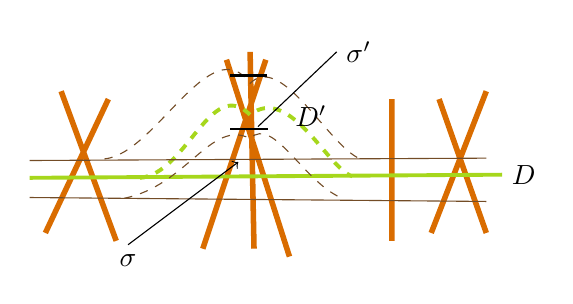
\begin{tikzpicture}[x=1cm,y=1cm]
\draw[orange!85!black,line width=2pt] (.2,-.7)--(1,1) (1.1,-.8)--(.4,1.1) (2.2,-.9)--(3,1.5) (3.3,-1)--(2.5,1.5) (2.85,-.9)--(2.8,1.6) (4.6,-.8)--(4.6,1) (5.1,-.7)--(5.8,1.1) (5.8,-.7)--(5.2,1);
\draw[yellow!65!green,line width=1.4pt] (0,0)--(6,.04);
\draw[yellow!65!green,line width=1.4pt,dashed] (1.4,0)..controls(2,.05)and(2.3,1.3)..(2.8,.8)..controls(3.3,1.2)and(3.8,.1)..(4.1,.02);
\draw[brown!60!black] (0,.22)--(5.8,.25) (0,-.25)--(5.8,-.3);
\draw[brown!60!black,dashed] (.95,.24)..controls(1.6,.3)and(2.3,1.9)..(2.8,1.2)..controls(3.2,1.6)and(3.8,.4)..(4.2,.24);
\draw[brown!60!black,dashed] (1.2,-.26)..controls(2,-.1)and(2.3,.75)..(2.8,.5)..controls(3.1,.8)and(3.5,-.1)..(4,-.27);
\draw[black,line width=1pt] (2.55,1.3)--(3.01,1.3) (2.55,.62)--(3.03,.62);
\draw[->] (1.25,-.85)--(2.65,.2);\node[below]at(1.25,-.85){$\sigma$};
\draw (3.9,1.6)--(2.9,.65);\node[right]at(3.9,1.6){$\sigma'$};
\node[right] at(6,.04){$D$};\node[right]at(3.25,.78){$D'$};
\end{tikzpicture}}

\uline{on trouve un isomorphisme canonique entre $\widehat P(D)$ et $\widehat P(D')$} transformant l'un des sommets $\sigma$ de $\widehat P(D)$ provenant de $\bar a$ en \deleted{\unsure{un}} l'un \uline{\unsure{antipodique}} \deleted{\unsure{que}} de l'un des sommets $\sigma'$ de $\widehat P(D')$ correspondant à $\bar a$. Une autre façon de le dire est celle-ci : Désignons par $a'$ l'arête de spécialisation ``opposée'' à $a$ (en $D'$), on trouve un isom des polygônes $\operatorname{Pol}(D)$ au \deleted{$\operatorname{Pol}(D')$,} \deleted{\unsure{un polygône}} \deleted{$\operatorname{Pol}(D')$, transformant} \deleted{\unsure{transformant en} $a$ \unsure{et l'image}} polygône déduit \deleted{\unsure{de}} de $\operatorname{Pol}(D')$ en retirant le sommet $a$, de sorte que $a$ aille sur $a'$.

\margin{\unsure{annulé;} cf plus bas !}

\deleted{Cet isomorp} \deleted{De plus,} on peut \inserted{donc} trouver un unique côté $\gamma$ de $D$, tel que le polygône \deleted{\unsure{déduit}} $\operatorname{Pol}'(D)$ déduit de $\operatorname{Pol}(D)$ en plaçant un point $a''$ dessus, soit isom. à $\operatorname{Pol}(D')$ par un isom prolongeant le précédent. De plus, cet isom est compatible avec les pondérations dans le sens suivant : deux \deleted{sommets} \inserted{sommets des polygônes (ou arêtes de $\Gamma(\underline\Sigma)$)} qui se correspondent ont $=$ pondérations (\unsure{en|on} donnant à $a''$ la pondération de $\alpha$), et aussi

\scanpage{21}
\margin{20}

\figure{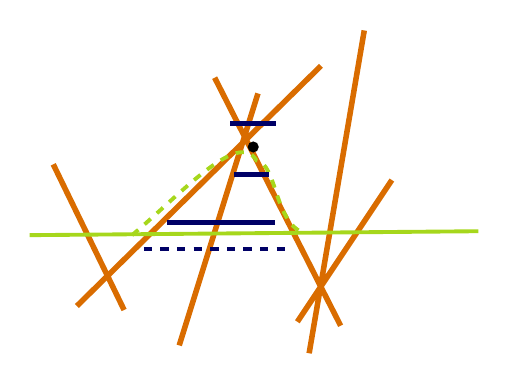
\begin{tikzpicture}[x=1cm,y=1cm]
\draw[orange!85!black,line width=2pt] (-1.4,-.9)--(1.7,2.15) (-1.7,.9)--(-.8,-.95) (-.1,-1.4)--(.9,1.8) (.35,2)--(1.95,-1.15) (1.55,-1.5)--(2.25,2.6) (1.4,-1.1)--(2.6,.7);
\draw[yellow!65!green,line width=1.4pt] (-2,0)--(3.7,.05);
\draw[yellow!65!green,line width=1.4pt,dashed] (-.7,0)..controls(-.1,.5)and(.65,1.35)..(.88,.95)..controls(1.15,.9)and(1.1,.15)..(1.5,.02);
\draw[blue!40!black,line width=1.6pt] (-.25,.16)--(1.12,.16) (.55,1.42)--(1.13,1.42) (.6,.77)--(1.04,.77);
\draw[blue!40!black,line width=1.4pt,dashed] (-.55,-.18)--(1.3,-.18);
\fill (.84,1.12) circle (2pt);
\end{tikzpicture}}

{\ttfamily\begin{tabular}{l}
\unsure{********************************************************************************}\\
*JESNEWS DU \unsure{03/08/1982|30/08/1982} C68 CADARACHE *\\
\unsure{********************************************************************************}\\
* DEPUIS LE 1/7/82 LES ALIAS DES COMMANDES LIBRARIAN *\\
* LIBGET (LG) ET LIBSAVE (LS) SONT SUPPRIMES, *\\
* POUR EVITER UNE POSSIBILITE DE CONFLIT AVEC *\\
* LE MEME ALIAS DES COMMANDES STANDARD IBM. *\\
* ******** *\\
* ATTENTION *\\
* MISE EN SERVICE LE VENDREDI 30/7/82 A 9H00 DE LA DEUXIEME PHASE DE GAF *\\
* SUR 168 CADARACHE. *\\
* ELLE PERMET D'UTILISER DANS LA CDE. KEEP TSO ET DANS LA PROCEDURE KEEP *\\
* BATCH UNE POSSIBILITE D'AFFECTATION DE TYPE DE SAUVEGARDE AU NIVEAU DU *\\
* FICHIER.CETTE POSSIBILITE EST VIVEMENT CONSEILLEE. *\\
* POUR PLUS AMPLES INFORMATIONS VOIR NOTE TECHNIQUE CISI MVS140,LA NOTE *\\
* MVS 145 ETANT SUPPRIMEE. *\\
* *\\
* EXEMPLES D'UTILISATION: *\\
* *\\
* BATCH: DSN=NOM.DU.FICHIER.A.SAUVEGARDER,DELAY=TYPE DE SAUVEGARDE *\\
* *\\
* TSO: *\\
* K DA('NOM DU FICHIER A SAUVEGARDER') DELAY(TYPE DE SAUVEGARDE) *\\
* *\\
* TYPES DE SAUVEGARDE: *\\
* *\\
* W SAUVEGARDE HEBDO. *\\
* D SAUVEGARDE JOURNALIERE. *\\
* NOS SAUVEGARDE MENSUELLE. *\\
* * PARAMETRE PAR DEFAUT. *\\
* *\\
\unsure{********************************************************************************}
\end{tabular}}

{\ttfamily\begin{tabular}{l}
\unsure{*******************************************************************}\\
* *\\
* - J E S N E W S F R 1 - LE 16/08/82 *\\
* *\\
*-----------------------------------------------------------------*\\
* *\\
* DEPUIS LE LUNDI 12 JUILLET 82, LES CLASSES DE TRAVAUX D ET E *\\
* SERONT ETENDUES POUR UNE TAILLE MEMOIRE SUPERIEURE A 1024 K *\\
* SE REPORTER A LA NOTE TECHNIQUE MVS141. *\\
* *\\
*-----------------------------------------------------------------*\\
* A PARTIR DU LUNDI 9 AOUT 1982, IL SERA POSSIBLE D'IMPRIMER *\\
* SUR XEROX 9700 (DESTINATION SAC) DES FICHIERS UTILISANT LE *\\
* COUPLE DE JEUX DE CARACTERES : (GS15,GT15) *\\
* *\\
*-----------------------------------------------------------------*\\
* *\\
* LE 16/08/82 : *\\
*------------- *\\
* -LE 370/168 SERA ARRETE DU VENDREDI 20 AOUT A 19H JUSQU'AU *\\
* LUNDI 23 AOUT A 8H.( MISE A NIVEAU TECHNIQUE.). *\\
* *\\
\unsure{*******************************************************************}
\end{tabular}}

\scanpage{22}
\mspage{10}
\margin{21}

deux secteurs angulaires (ou arêtes de $\operatorname{Pol}'(D)$, $\operatorname{Pol}(D')$) quand celles en $D$ sont pondérées, i.e. à l'exception \unsure{des deux cas des} arêtes \deleted{\unsure{de}} $\alpha,\beta$ \deleted{\unsure{des demi-arêtes}} qui découpent l'arête $\gamma$, et qui ne sont pas encore pondérées. La formule des pondérations implique alors qu'on doit avoir, pour les arêtes $\alpha',\beta'$ correspondantes de $\operatorname{Pol}(D')$
\[
\deleted{\operatorname{poids}(\alpha')+\operatorname{poids}(a'')+}
\]
\[
\operatorname{poids}(\alpha')+\operatorname{poids}(\beta')+\operatorname{poids}(a)=\operatorname{poids}(\gamma)
\]

\uline{NB} Il est commode d'augmenter le polygône $\operatorname{Pol}(D)$ en $\unsure{\overline{\operatorname{Pol}}(D)^*}$, en rajoutant, en tt sommet \deleted{\unsure{qui ne}} \inserted{correspondant} à une arête de spécialisation \deleted{\unsure{quelconque}} $a:D\mathbin{-}D'$ de $\Gamma(\underline\Sigma)$, une ``antipodique'' mais considérée comme arête \deleted{\unsure{orientée}} à bout libre (ayant une origine, mais pas d'extrémité) --- ceci ne rajoute pas d'autres sommets à $\Gamma(\underline\Sigma)$, seult des arêtes libres. Mais tte flèche de spécialisation $D\to D'$ induit un iso
\[
P^*(D)\mathbin{-}P^*(D')
\]

\figure{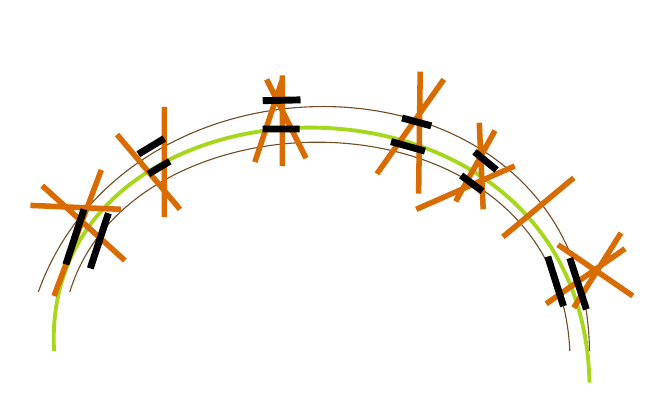
\begin{tikzpicture}[x=1cm,y=1cm]
\draw[yellow!65!green,line width=1.4pt] (-3.5,-.5)..controls(-3.7,3.2)and(3.2,3.5)..(3.3,-.9);
\draw[brown!60!black] (-3.7,.25)..controls(-2.5,3.6)and(3.25,3.4)..(3.3,-.5);
\draw[brown!60!black] (-3.3,.25)..controls(-2.5,2.9)and(2.9,2.9)..(3.05,-.5);
\draw[orange!85!black,line width=2pt] (-3.5,.2)--(-2.9,1.8) (-3.65,1.6)--(-2.6,.65) (-3.8,1.35)--(-2.65,1.3);
\draw[orange!85!black,line width=2pt] (-2.1,1.2)--(-2.1,2.6) (-2.7,2.25)--(-1.9,1.3);
\draw[orange!85!black,line width=2pt] (-.95,1.9)--(-.6,2.95) (-.6,1.85)--(-.6,3) (-.3,1.95)--(-.8,2.95);
\draw[orange!85!black,line width=2pt] (.6,1.75)--(1.45,2.95) (1.13,1.5)--(1.15,3.05);
\draw[orange!85!black,line width=2pt] (1.6,1.4)--(2.1,2.3) (1.95,1.3)--(1.9,2.4) (1.1,1.3)--(2.35,1.85);
\draw[orange!85!black,line width=2pt] (2.2,.95)--(3.1,1.7);
\draw[orange!85!black,line width=2pt] (2.75,.1)--(3.75,.8) (3.1,.05)--(3.7,1) (2.9,.85)--(3.85,.2);
\draw[black,line width=2.5pt] (-3.35,.6)--(-3.12,1.3) (-3.04,.55)--(-2.81,1.25) (-2.43,2)--(-2.1,2.2) (-2.3,1.75)--(-2.03,1.91) (-.85,2.68)--(-.37,2.69) (-.85,2.32)--(-.38,2.32) (.92,2.46)--(1.29,2.36) (.78,2.16)--(1.21,2.04) (1.84,2.03)--(2.12,1.8) (1.67,1.73)--(1.94,1.53) (3.05,.68)--(3.26,.03) (2.77,.7)--(2.97,.07);
\end{tikzpicture}}

La réflexion en termes de $P(D)\mathbin{-}P(D')$ est trompeuse, en effet \unsure{par} \inserted{\unsure{en le|dans le} triangle $T$ spécialisation} les triangles de spécialisation (\unsure{non}, en dehors \inserted{s'il y en a} attenant à $T$ \deleted{peuvent} \inserted{sont} disponibles comme tels --- il faudrait donc indiquer la \uline{relation d'adjacence} des triangles de spécialisation de \deleted{$\unsure{\Gamma(\underline\Sigma)}$} $D$, comme faisant partie de la structure de $\Gamma(\underline\Sigma)$ ---

\margin{\uline{NB} elle est déterminée en fait par la structure des pondérations.}

\figure{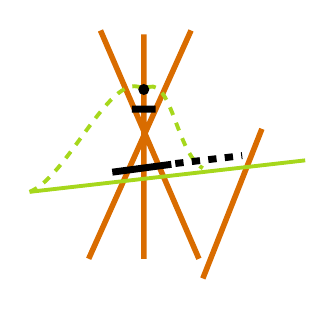
\begin{tikzpicture}[x=1cm,y=1cm]
\draw[orange!85!black,line width=2pt] (-.65,-1.25)--(.65,1.65) (.75,-1.25)--(-.5,1.65) (.05,-1.25)--(.05,1.6) (.8,-1.5)--(1.55,.4);
\draw[yellow!65!green,line width=1.4pt] (-1.4,-.4)--(2.1,0);
\draw[yellow!65!green,line width=1.4pt,dashed] (-1.4,-.4)..controls(-.9,-.2)and(-.35,1.2)..(.05,.9)..controls(.4,1.15)and(.45,.1)..(.8,-.1);
\fill (.05,.9) circle (2pt);
\draw[black,line width=2.5pt] (-.1,.65)--(.2,.65) (-.35,-.15)--(.4,-.05);
\draw[black,line width=2.5pt,dashed] (.45,-.04)--(1.3,.06);
\end{tikzpicture}}

et la structure supplémentaire s'obtiendrait en collant d'abord au $\operatorname{Pol}(D)$ les triangles de spécialisation (s'il y en a) qui sont attenants à $T$, soit $\operatorname{Pol}(D,\unsure{a})$ \deleted{\unsure{Ce}} ce nouveau polygône. On peut aussi, \unsure{tout autant}, augmenter \deleted{$\operatorname{Pol}$} $\operatorname{Pol}(D)$, \deleted{$\operatorname{Pol}(D')$}, en y incluant des arcs des \unsure{faux bords} des ``pseudo-triangles de spécialisation'', dont

\margin{oui, et semble plus élégant}

\scanpage{23}
\mspage{11}
\margin{22}

une des extrémités serait un sommet de $\Sigma$, comme

\figure{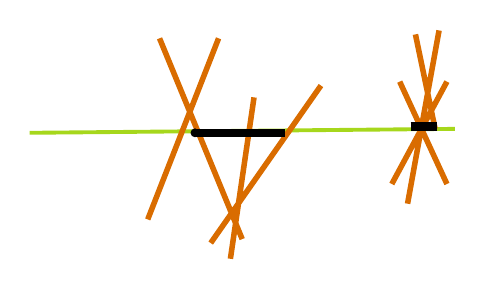
\begin{tikzpicture}[x=1cm,y=1cm]
\draw[yellow!65!green,line width=1.4pt] (-2.2,0)--(3.2,.05);
\draw[orange!85!black,line width=2pt] (-.7,-1.1)--(.2,1.2) (.5,-1.35)--(-.55,1.2) (.35,-1.6)--(.65,.45) (.1,-1.4)--(1.5,.6) (2.4,-.65)--(3.1,.65) (3.1,-.65)--(2.5,.65) (2.6,-.9)--(3,1.3) (2.95,.05)--(2.7,1.25);
\draw[black,line width=3pt] (-.1,0)--(1.04,0) (2.64,.08)--(2.97,.08);
\fill(-.1,0)circle(1.6pt);
\end{tikzpicture}}

(on lui fait correspondre une arête libre de $\Gamma(\underline\Sigma)$, sans autre sommet au bout); \uline{il serait pratique} d'inclure, comme dit plus haut, les antipodiques de \inserted{ts} ces arcs (de spécialisation, ou de pseudo-spécialisation --- pour un arc de vraie spécialisation, \deleted{\unsure{il en est}} l'antipodique est \unsure{soit} de spécialisation, soit de pseudo-spécialisation) --- également en bouts libres. Soit $\operatorname{Pol}^*(D)$ ce polygône (plus grand que celui précédemment désigné sous ce vocable). On trouve alors un \deleted{\unsure{bon}} iso de $\operatorname{Pol}^*(D)$ avec un \uline{sous-polygône} de $\operatorname{Pol}^*(D')$, mais ce n'est pas néc. un iso, car de nouveaux arcs de pseudo-spécialisation \inserted{(ou triangles)} $t$ peuvent être créés par spécialisation, dans le cas où l'une ou l'autre des deux faces adjacentes au triangle $T$ sur l'une de ses \unsure{deux} faces latérales est un carré. Donc \unsure{il peut alors y avoir} deux \inserted{\unsure{voisins de}} sommets \inserted{\unsure{contigus}} dans l'image de

\figure{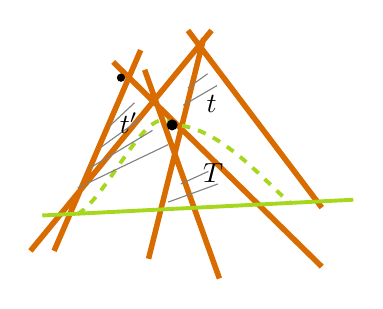
\begin{tikzpicture}[x=1cm,y=1cm]
\coordinate(A)at(0,1.1);\coordinate(B)at(-.65,1.7);\coordinate(C)at(.35,2.05);
\draw[orange!85!black,line width=2pt] (-1.8,-.5)--(.5,2.3) (-1.5,-.5)--(-.4,2.05) (-.75,1.9)--(1.9,-.7) (-.3,-.6)--(.4,2.2) (.6,-.85)--(-.35,1.8) (.2,2.3)--(1.9,.05);
\draw[yellow!65!green,line width=1.4pt] (-1.65,-.05)--(2.3,.15);
\draw[yellow!65!green,line width=1.4pt,dashed] (-1.2,-.03)..controls(-.8,.2)and(-.3,1.45)..(0,1.1)..controls(.6,1.1)and(1.2,.35)..(1.5,.11);
\draw[gray] (-1.2,.3)--(-.05,.85) (-1.05,.55)--(-.25,1.03) (-.9,.82)--(-.4,1.18) (-.8,1.08)--(-.48,1.38) (.14,1.35)--(.57,1.6) (.2,1.57)--(.45,1.75) (.11,.35)--(.46,.51) (-.05,.12)--(.58,.35);
\fill(A)circle(2pt);\fill(B)circle(1.5pt);
\node at(-.55,1.12){$t'$};\node at(.5,1.37){$t$};\node at(.52,.49){$T$};
\end{tikzpicture}}

\figure{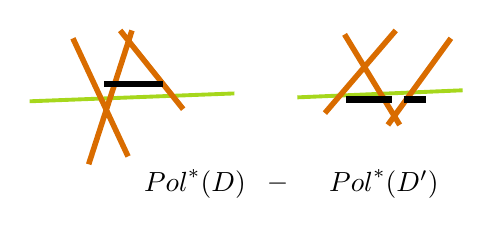
\begin{tikzpicture}[x=1cm,y=1cm]
\draw[yellow!65!green,line width=1.4pt] (-1.1,0)--(1.5,.1) (2.3,.05)--(4.4,.14);
\draw[orange!85!black,line width=2pt] (-.35,-.8)--(.2,.9) (.15,-.7)--(-.55,.8) (.05,.9)--(.85,-.1) (2.65,-.15)--(3.55,.9) (3.6,-.3)--(2.9,.85) (3.45,-.3)--(4.25,.8);
\draw[black,line width=2.5pt] (-.15,.22)--(.6,.22) (2.92,.02)--(3.5,.02) (3.65,.02)--(3.94,.02);
\node at(1,-1.05){$\operatorname{Pol}^*(D)$};\node at(2.05,-1.05){$-$};\node at(3.4,-1.05){$\operatorname{Pol}^*(D')$};
\end{tikzpicture}}

\margin{\uline{NB} la pondération du polygône $\operatorname{Pol}^*(D)$ est stable par antipodie.}

L'introduction de $\operatorname{Pol}^*(D)$ est intéressante, puisqu'elle est stable par antipodisme. Si on veut exprimer la compatibilité avec les pondérations, on dira que deux \deleted{arêtes} \inserted{sommets} qui se correspondent ont $=$ pondérations, ainsi que deux arêtes qui se correspondent. Quand $\operatorname{Pol}^*(D)\mathbin{-}\operatorname{Pol}^*(D')$ n'est pas un iso, alors il y a \deleted{les} un ou deux des sommets adjacents \deleted{aux} aux sommets $(D',a)$, $(D',a')$ de $\operatorname{Pol}^*(D')$ qui manquent.

\margin{\uline{NB} La pondération d'une \uline{arête} de $\operatorname{Pol}^*(D)$ peut être nulle --- \deleted{p.ex} entre \deleted{\unsure{deux adjacents}} \inserted{un} arc de \deleted{spécialisation} générisation, \unsure{et} un arc de ps.-spéc. adjacent cf figure ci dessus et aussi entre l'antip. d'un arc de spéc et un autre arc de spécialisation.}

\scanpage{24}
\mspage{12}
\margin{23}

\figure{\begin{tikzpicture}[x=1cm,y=1cm]
\draw (-2.3,-.15)..controls(-1.2,.9)and(1.3,.8)..(2.4,-.35);
\draw (-2,.02)--(-2.05,.15) (-1.15,.48)--(-1.18,.61) (-.1,.56)--(-.12,.65);
\node[above]at(-2.05,.17){$x$};\node[above]at(-1.18,.62){$b$};\node[above]at(-.12,.66){$a$};
\end{tikzpicture}}

Si $b$ manque ds $\operatorname{Pol}^*(D)$, et sur l'arc $\overset{\frown}{ax}$ de $\operatorname{Pol}^*(D')$, ($x$ étant l'autre sommet de $\operatorname{Pol}^*(D')$ adjacent à $b$) on doit avoir
\[
\begin{aligned}
&\text{pondération de $\overset{\frown}{a,x}$ dans $\operatorname{Pol}^*(D)$}\\
&\qquad=\text{somme des pondérations de}\\
&\qquad\overset{\frown}{x,b},\ b,\ \overset{\frown}{b,a}\text{ dans }\operatorname{Pol}^*(D').
\end{aligned}
\]
[Pour exprimer commodément cette \unsure{égalité}, il faudrait développer la notion de pondération d'un sous-polygône d'un polygône pondéré, \deleted{\unsure{de}} de telle façon que les déploiements du polygône \inserted{pondéré} initial et du sous-polygône soient can. isom.]

La question se pose si les \deleted{\unsure{deux}} applications $\operatorname{Pol}^*(D)\mathbin{-}\operatorname{Pol}^*(D')$ peuvent se déduire des autres structures de $\Gamma^*(\underline\Sigma)$ (\deleted{\unsure{par structure}} cellularisation et \deleted{\unsure{la}} pondération).

Il faudrait d'abord passer en revue les \unsure{structures|structure} des \unsure{polygônes|polygône} $\operatorname{Pol}^*(D)$ (en d'abord $D$ non supercritique).

a) Parmi ses sommets, \deleted{il y a les} i.e. les arêtes de $\Gamma^*(\unsure{\underline\Sigma|D})$ en $D$, il y a les sommets de \uline{spécialisation} (arêtes \deleted{\unsure{entrantes}} \inserted{partant} de $D$), les arêtes de générisation (ce sont celles arrivant à $D$), et enfin les sommets neutres (arêtes libres en $D$, non-topologiques, arêtes dont l'autre extrémité est un ``bout'' au sens d'avant). Notons

a) L'ens des \deleted{arêtes} \inserted{sommets (ou arêtes)} de générisation est stable par l'antipodisme.

b) Si $a$ est une \deleted{arête} \inserted{sommet} de spécialisation, son antipodique n'est pas \deleted{arête} \inserted{sommet} de spécialisation.

c) Une \deleted{arête} \inserted{sommet} qui n'est ni \deleted{arête} de générisation, ni de spécialisation, ni antipodique d'une telle \inserted{(ou les deux)} est donc soit une ps. spécialisation, soit antipodique d'une telle, ce qui \unsure{implique} \inserted{au moins} qu'il est adjacent à un sommet de générisation, et la pondération de l'arête qui les joint est nulle, et réciproquement

\figure{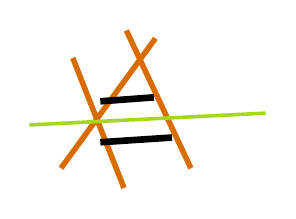
\begin{tikzpicture}[x=1cm,y=1cm]
\draw[orange!85!black,line width=2pt] (-.7,-.55)--(.5,1.1) (.1,-.8)--(-.55,.85) (.95,-.55)--(.13,1.2);
\draw[yellow!65!green,line width=1.3pt] (-1.1,0)--(1.9,.15);
\draw[black,line width=2.4pt] (-.2,.3)--(.48,.35) (-.2,-.22)--(.71,-.16);
\end{tikzpicture}}

\scanpage{25}
\mspage{13}
\margin{24}

Il ne semble pas que la structure de graphe orienté cellularisé pondéré de $\Gamma^*(\underline\Sigma)$ permette de distinguer, parmi les \deleted{sommets} arêtes issues d'un sommet $D$ i.e. les sommets de $\operatorname{Pol}^*(D)$, celles et ceux qui correspondent à des triangles de ps. spécialisation (parmi les \deleted{\unsure{paires de sommets}} \inserted{sommets incidents} à des arêtes \deleted{\unsure{de poids}} de $\operatorname{Pol}^*(D)$ de poids nul, dont \deleted{\unsure{l'antipodique est un sommet}} l'un au moins soit sommet de générisation).

\margin{mais si ! cf ci-contre !}

Cette distinction peut se déduire si on dispose des applications de spécialisation \deleted{\unsure{et des}} $\operatorname{Pol}^*(D)\longrightarrow\operatorname{Pol}^*(D')$ : les sommets de ps. spécialisation sont distingués, parmi les précédents, comme \deleted{aux} les ``spécialisés'' des sommets de spécialisation véritables.

La prochaine question est donc si les applications de spécialisation
\[
\operatorname{Pol}^*(D)\longrightarrow\operatorname{Pol}^*(D')
\]
sont déductibles des structures précédentes. \uline{Mais bien sûr}, via l'\deleted{effet} isom correspondant sur les polygônes déployés, car il suffit de

\unsure{a)} savoir \unsure{qu'ils sont} de $=$ ordre (\unsure{calculable|découle})

b) de savoir \deleted{l'effet} du morphisme sur l'ens des deux orientations, ce qui est connu, et

c) de savoir l'image d'un sommet particulier \inserted{$(D,a)$} de $\widehat{\operatorname{Pol}}^*(D)$, qui est \unsure{connu} comme l'antipodique, dans $\widehat{\operatorname{Pol}}(D')$, du sommet $(D',a)$ !

En fait, chaque fois qu'on a une 2-carte \inserted{(avec bouts isolés i.e. arêtes libres)} dont les \deleted{\unsure{deux}} (vrais) sommets sont d'ordre $2$, et dont les arêtes et coins sont pondérés [avec pondérations des arêtes $\ge0$], \deleted{\unsure{et où}} et la pondération totale de chaque sommet \deleted{est} (somme des pondérations des \deleted{\unsure{inc}} \inserted{arcs} et coins incidents) est cte, on trouve des isom de transport entre les polygônes locaux déployés, qui forment donc un syst. local sur la surface sous-jacente à la carte !

\scanpage{26}
\mspage{14}
\margin{25}

Dans le cas actuel, il se trouve que cet iso. des \unsure{deux pol.} \deleted{\unsure{déployés|définis}} \inserted{\unsure{en question}} pour induire \unsure{de lui-même} $\operatorname{Pol}^*(D)\longrightarrow\operatorname{Pol}^*(D')$ ayant les propriétés \unsure{signalées}.

Il faudrait examiner à part la situation de spécialisation vers un $\Delta$ supersingulier.

24.12. Finalement, il apparaît que c'est le polygône $\unsure{\operatorname{Pol}^{\wedge}(D)|\operatorname{Pol}^{*}(D)}$ qui est ``le bon'', ou encore mieux, le polygône dual ; \unsure{le passage} \deleted{\unsure{d'un}} au dual revient à passer à la carte \uline{duale} de celle considérée hier --- c'est la carte duale qui est la plus intuitive encore. À partir \unsure{des|de} positions relatives, on visualise le polygône \unsure{dual} $\operatorname{Pol}(D)$ (\unsure{nouvelle} \unsure{version|dessin} !) comme \deleted{le bord} associé au pôle $D$, bord d'un petit voisinage tubulaire autour de $D$, ou encore bord du disque $\Delta(D)$ fermé complt de l'intérieur de ce voisinage tubulaire, et la carte qui nous intéresse peut être considérée comme obtenue en recollant les disques $\Delta(D)$, d'une façon naturelle que je viens de \unsure{m'expliquer} --- ou plutôt, \deleted{\unsure{ce}} qu'on déduit de ces disques en prenant \inserted{pour chaque $\Delta(D)$} sur le bord les ``arêtes libres'' (i.e. celles qui ne sont arêtes de spécialisation ni de générisation) \inserted{marquées en vert et bleu ici}, et en les repliant par le milieu, de sorte qu'on trouve un disque \inserted{$\Delta'(D)$} dans lequel les arêtes \inserted{repliées} précédentes apparaissent comme \inserted{autant de} segments allant du bord vers l'intérieur. Si on garde le tracé du \deleted{\unsure{le}} syst. de droites (en rouge) à l'intérieur de $\Delta'(D)$ (cf figure ci-contre, voisinage du bord) \unsure{on donne|on dénoue} des points doubles

\figure{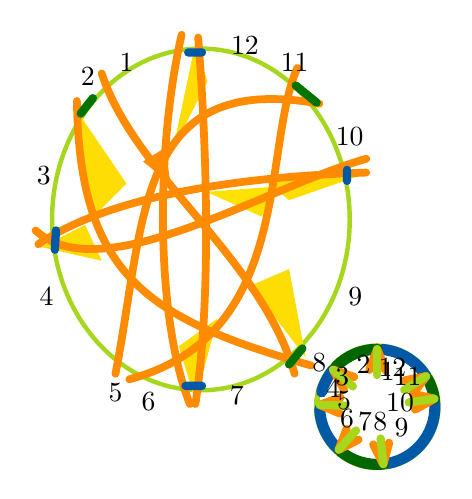
\begin{tikzpicture}[x=0.7cm,y=0.7cm,line cap=round,line join=round]
\draw[yellow!65!green,line width=1.6pt] (0,0) ellipse (2.7 and 3.1);
\fill[yellow!80!orange] (-.1,3.2)--(-.5,1.3)--(.12,2.5)--cycle;
\fill[yellow!80!orange] (-2.2,1.9)--(-2,0)--(-1.35,.65)--cycle;
\fill[yellow!80!orange] (-2.9,-.5)--(-1.8,-.75)--(-2.1,-.1)--cycle;
\fill[yellow!80!orange] (-.1,-3.3)--(.3,-1.8)--(-.4,-2.3)--cycle;
\fill[yellow!80!orange] (1.9,-2.5)--(.9,-1.2)--(1.6,-.9)--cycle;
\fill[yellow!80!orange] (2.9,.8)--(1.1,.75)--(1.6,.35)--cycle;
\fill[orange!90!yellow] (-.65,1.3)--(-1.05,1.05)--(-.55,.65)--cycle;
\fill[yellow!85!orange] (.1,.5)--(1.1,.05)--(1.4,.6)--cycle;
\draw[orange!90!yellow,line width=2.8pt] (-2.25,2.15) .. controls (-2.2,-1) and (-1,-1.8) .. (2,-2.65);
\draw[orange!90!yellow,line width=2.8pt] (-1.8,2.65) .. controls (-1.2,.8) and (1.1,-.7) .. (1.7,-2.8);
\draw[orange!90!yellow,line width=2.8pt] (-.35,3.35) .. controls (-.8,1.4) and (-.85,-1.7) .. (-.2,-3.35);
\draw[orange!90!yellow,line width=2.8pt] (-.05,3.3) .. controls (.1,1.4) and (.2,-1.4) .. (-.1,-3.35);
\draw[orange!90!yellow,line width=2.8pt] (-2.95,-.45) .. controls (-1.4,.6) and (1.5,.8) .. (3,.85);
\draw[orange!90!yellow,line width=2.8pt] (-3,-.2) .. controls (-1.8,-1.3) and (1.2,.6) .. (3,1.1);
\draw[orange!90!yellow,line width=2.8pt] (-1.55,-2.8) .. controls (-1,0) and (-1.2,2.7) .. (2.15,2.1);
\draw[orange!90!yellow,line width=2.8pt] (-1.3,-2.9) .. controls (1.7,-2.1) and (1.1,1.3) .. (1.75,2.75);
\draw[blue!65!green,line width=3pt] (-2.65,-.55)--(-2.63,-.2) (-.28,-3.02)--(.02,-3.02) (2.65,.7)--(2.65,.9) (-.23,3.03)--(.02,3.03);
\draw[green!45!black,line width=3pt] (-2.18,1.92)--(-1.96,2.2) (1.72,2.43)--(2.1,2.12) (1.6,-2.63)--(1.84,-2.34);
\node at (-1.35,2.85) {$\unsure{1}$};\node at (-2.05,2.6) {$\unsure{2}$};\node at (-2.85,.8) {$3$};\node at (-2.8,-1.4) {$4$};\node at (-1.55,-3.15) {$5$};\node at (-.95,-3.3) {$6$};\node at (.65,-3.2) {$7$};\node at (2.15,-2.6) {$8$};\node at (2.8,-1.4) {$9$};\node at (2.7,1.5) {$10$};\node at (1.7,2.85) {$\unsure{11}$};\node at (.8,3.15) {$12$};
\begin{scope}[shift={(3.2,-3.4)},scale=.55]
\draw[yellow!65!green,line width=2pt] (0,0) circle (2);
\draw[blue!65!green,line width=4pt] (85:1.9) arc(85:32:1.9) (7:1.9) arc(7:-80:1.9) (-132:1.9) arc(-132:-178:1.9) (165:1.9) arc(165:140:1.9);
\draw[green!40!black,line width=4pt] (136:1.9) arc(136:90:1.9) (30:1.9) arc(30:8:1.9) (-84:1.9) arc(-84:-130:1.9);
\foreach \a in {90,140,178,-132,-84,8,32}{\draw[orange!90!yellow,line width=3pt] (\a:1.9)--({\a-12}:1.25) (\a:1.9)--({\a+12}:1.25);\draw[yellow!65!green,line width=3pt] (\a:1.9)--(\a:1.05);}
\node at (.35,1.15) {$1$};\node at (-.45,1.4) {$2$};\node at (-1.15,1) {$3$};\node at (-1.45,.6) {$4$};\node at (-1.1,.2) {$5$};\node at (-1,-.4) {$6$};\node at (-.4,-.5) {$7$};\node at (.1,-.5) {$8$};\node at (.8,-.7) {$9$};\node at (.75,.15) {$10$};\node at (1,1) {$11$};\node at (.5,1.3) {$\unsure{12}$};
\end{scope}
\end{tikzpicture}}

\scanpage{27}
\margin{26}
\figure{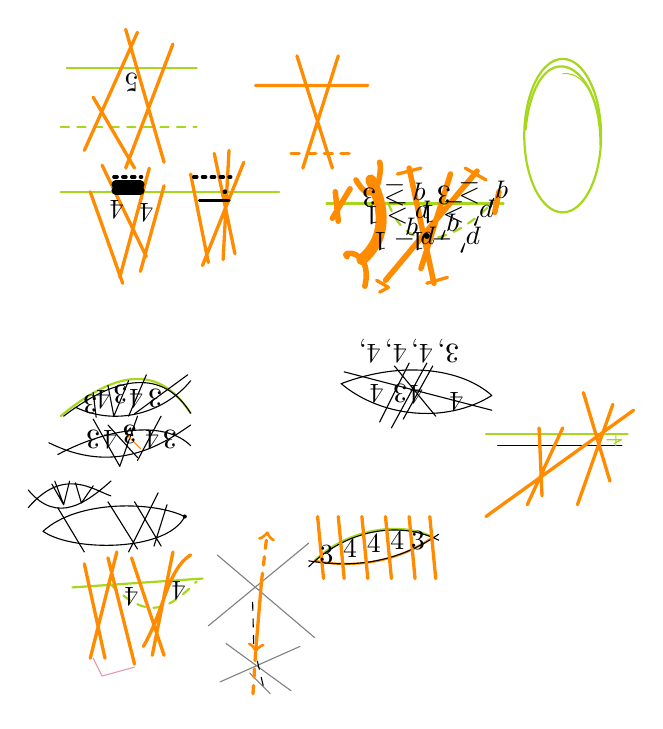
\begin{tikzpicture}[x=.75cm,y=.75cm,line cap=round,line join=round]
\begin{scope}[shift={(0,0)}]
\draw[yellow!65!green,thick] (-1.1,.8)--(1.1,.8);\draw[yellow!65!green,thick,dashed] (-1.2,-.2)--(1.1,-.2);
\draw[orange!90!yellow,very thick] (-.8,-.6)--(.1,1.4) (-.1,1.45)--(.55,-.8) (-.65,.3)--(.05,-.9) (-.1,-.9)--(.7,1.2);
\node[rotate=180] at (0,.55) {$5$};
\end{scope}
\begin{scope}[shift={(3,0)}]
\draw[orange!90!yellow,very thick] (-.9,.5)--(1,.5) (-.2,1)--(.4,-.9) (.5,1)--(-.1,-.9);\draw[orange!90!yellow,very thick,dashed] (-.3,-.65)--(.7,-.65);
\end{scope}
\begin{scope}[shift={(7.3,-.35)}]
\draw[yellow!65!green,thick] (0,0) ellipse(.65 and 1.3);\draw[yellow!65!green,thick] (-.63,.1) .. controls (-.45,1.8) and (.65,1.3) .. (.64,-.15);\draw[yellow!65!green] (0,1.05) .. controls (.45,1.1) and (.65,.4) .. (.65,-.1);
\end{scope}
\begin{scope}[shift={(0,-2)}]
\draw[yellow!65!green,thick] (-1.2,.7)--(2.5,.7);
\draw[orange!90!yellow,very thick] (-.5,1.15)--(.25,-.4) (.3,1.1)--(-.2,-.75) (-.7,.7)--(-.15,-.85) (.55,.8)--(.15,-.65);
\draw[line width=3pt] (-.27,.72)--(.15,.72) (-.27,.82)--(.15,.82);\draw[very thick,dotted] (-.3,.95)--(.17,.95);
\node[rotate=180] at (-.25,.4) {$4$};\node[rotate=180] at (.25,.35) {$4$};
\draw[orange!90!yellow,very thick] (1,1)--(1.3,-.5) (1.4,1.35)--(1.75,-.35) (1.65,1.4)--(1.55,-.45) (1.9,1.2)--(1.2,-.55);
\fill (1.58,.7) circle(.04);\draw[very thick] (1.15,.55)--(1.65,.55);\draw[very thick,dotted] (1.05,.95)--(1.68,.95);
\end{scope}
\begin{scope}[shift={(5,-2.2)}]
\draw[yellow!65!green,thick] (-1.7,.7)--(1.3,.7);\draw[yellow!65!green,thick,dashed] (-.65,.7)..controls(-.3,-.25)and(.5,.1)..(1.1,.7);
\draw[orange!90!yellow,line width=2pt] (-1.6,.45)--(-1.3,.95) (-1.55,.9)--(-1.5,.4) (-.3,1.3)--(.12,-.65) (-.7,-.6)--(.85,1.25) (-.1,-.4)--(.4,1.2) (1.15,.55)--(1.22,.9);
\draw[orange!90!yellow,line width=2pt] (-1.2,1.1)..controls(-.85,.5)and(-.75,1.3)..(-.8,1.4) (-1.05,-.7)..controls(-.9,-.05)and(-1.5,-.1)..(-1.35,-.2);
\draw[orange!90!yellow,line width=4pt] (-.95,1.1)..controls(-.65,.5)and(-.75,.05)..(-1.1,-.25);
\draw[orange!90!yellow,very thick] (-.5,1.2)--(-.1,1.3) (.65,1.3)--(1,1.1) (-.85,-.6)--(-.65,-.72)--(-.8,-.8) (0,-.65)--(.35,-.55);
\fill (0,.15) circle(.05);
\node[rotate=180] at (-.38,.1) {$p-1$};\node[rotate=180] at (-.25,.3) {$q$};\node[rotate=180] at (-.5,.55) {$p\ge1$};\node[rotate=180] at (-.55,.85) {$q\ge3$};
\node[rotate=180] at (.32,.08) {$p'-1$};\node[rotate=180] at (.38,.3) {$q'$};\node[rotate=180] at (.52,.53) {$p'\ge1$};\node[rotate=180] at (.78,.85) {$q'\ge3$};
\end{scope}
\begin{scope}[shift={(0,-5.1)}]
\draw[yellow!65!green,thick] (-1.2,0)..controls(0,1)and(.6,.65)..(1,.05);\draw (-1.15,0)..controls(-.1,.8)and(.6,.7)..(1,.05) (-.95,.15)..controls(-.2,-.2)and(.6,.1)..(1,.6);
\draw (-.6,-.02)--(-.65,.4) (-.3,0)--(-.4,.52) (-.3,0)--(-.05,.6) (-.05,0)--(.25,.7) (.05,.04)--(.95,.7);
\foreach \x/\y/\v in {-.7/.2/3,-.48/.28/4,-.19/.36/3,.08/.3/4,.4/.3/3}{\node[rotate=180] at(\x,\y){$\v$};}
\end{scope}
\begin{scope}[shift={(4.8,-4.8)}]
\draw (-1.25,.25)..controls(-.2,.65)and(.8,.5)..(1.3,.05)..controls(.5,-.45)and(-.6,-.3)..cycle;
\draw (-1.2,.45)--(1.3,-.2) (-.35,.55)--(.35,-.3) (-.1,.6)--(-.6,-.4) (.2,.6)--(-.4,-.5) (.3,.55)--(-.2,-.35);
\foreach \x/\y/\v in {-.65/.08/4,-.25/.08/3,.02/.07/4,.7/-.05/4}{\node[rotate=180] at(\x,\y){$\v$};}\node[rotate=180] at (-.1,.8) {$3,4,4,4,$};
\end{scope}
\begin{scope}[shift={(7.2,-5.7)}]
\draw[yellow!65!green,thick] (-1.2,.3)--(1.2,.3);\draw (-1,.1)--(1.1,.1);
\draw[orange!90!yellow,very thick] (-1.2,-1.1)--(1.3,.7) (.45,1)--(.9,-.5) (.95,.8)--(.35,-.9) (-.3,.4)--(-.25,-.75) (.1,.4)--(-.5,-.9);
\draw[yellow!65!green] (1,.3)--(1,.1) (.85,.2)--(1.1,.2)--(.97,.14);
\end{scope}
\begin{scope}[shift={(0,-5.9)}]
\draw (-1.25,.15)..controls(-.3,.65)and(.6,.7)..(1,.3) (-1.4,.35)..controls(-.3,-.2)and(.5,.3)..(1,.65);
\draw (-.65,.75)--(-.2,-.05) (-.4,.65)--(.1,.1) (-.2,-.05)--(.1,.8) (.1,.05)--(.5,.8);
\draw[orange] (-.1,.5)--(.15,.25);\draw (-.1,.5)--(-.02,.6)--(.02,.47)--cycle;
\foreach \x/\v in {-.65/3,-.36/4,.35/4,.65/3}{\node[rotate=180]at(\x,.4){$\v$};}\node[rotate=180]at(-.03,.49){$\unsure{3}$};
\end{scope}
\begin{scope}[shift={(-.75,-6.65)}]
\draw (-1,0)..controls(-.4,.7)and(.1,.3)..(.4,.2) (-1,.3)..controls(-.5,-.3)and(0,.1)..(.4,.45);
\draw (-.6,.4)--(-.4,.05)--(-.3,.45) (-.4,.05)--(-.55,.45) (-.2,.42)--(-.1,.08)--(.1,.37);
\end{scope}
\begin{scope}[shift={(-.1,-7.2)}]
\draw (-1.4,.15)..controls(-.8,.7)and(.5,.65)..(1,.4)..controls(.7,-.2)and(-.9,-.2)..cycle;
\draw (-1.15,.55)--(-.7,-.2) (-.3,.65)--(.2,-.15) (.15,.65)--(.6,-.1) (.05,-.2)--(.55,.8) (.48,-.1)--(.7,.6);\fill(1,.4)circle(.035);
\end{scope}
\begin{scope}[shift={(4.1,-7.15)},rotate=180]
\draw[yellow!65!green,thick] (-1,0)..controls(-.4,-.3)and(.5,-.1)..(1,.4);\draw[orange!90!yellow,thick] (-1,0)..controls(-.3,.5)and(.5,.5)..(1,.4);
\draw (-1.1,-.05)..controls(-.3,.5)and(.5,.5)..(1.1,.4) (-1.1,.05)..controls(-.4,-.3)and(.5,-.1)..(1.1,.5);
\foreach \x in {-.95,-.6,-.2,.2,.6,.95}{\draw[orange!90!yellow,very thick] (\x,-.35)--({\x-.1},.7);}
\foreach \x/\y/\v in {-.75/.05/3,-.4/.05/4,0/.1/4,.4/.2/4,.8/.3/3}{\node at(\x,\y){$\v$};}
\end{scope}
\begin{scope}[shift={(0,-8.5)}]
\draw[yellow!65!green,thick] (-1,.5)--(1.2,.65);\draw[yellow!65!green,dashed,thick] (-.35,.55)..controls(.3,-.1)and(.65,.15)..(1.1,.6);
\draw[orange!90!yellow,very thick] (-.8,.9)--(-.45,-.7) (-.25,1.1)--(-.7,-.7) (-.4,1)--(.05,-.8) (0,1)--(.55,-.65) (.7,1.1)--(.35,-.65) (.2,-.5)..controls(.55,.1)and(.6,.8)..(1,1.05);
\draw[purple!40] (-.65,-.7)--(-.5,-1)--(.05,-.85);\node[rotate=180]at(0,.35){$\unsure{4}$};\node[rotate=180]at(.8,.45){$\unsure{4}$};
\end{scope}
\begin{scope}[shift={(2.2,-8.45)}]
\draw[gray] (-.75,1)--(.9,-.4) (-.9,-.2)--(.8,1.2) (-.7,-1.15)--(.65,-.55) (-.6,-.5)--(.5,-1.3) (-.2,-1)--(.15,-1.35);
\draw[orange!90!yellow,very thick,->] (0,.55)--(-.1,-.65);\draw[orange!90!yellow,very thick,dashed,->] (0,.55)--(.1,1.4);\draw[orange!90!yellow,very thick,dashed] (-.1,-.65)--(-.15,-1.45);\draw[black,dashed] (-.15,.2)--(-.13,-.6) (-.07,-.8)--(.05,-1.3);
\end{scope}
\end{tikzpicture}}

\texttt{//*\quad CRAY2\quad 0352\qquad \unsure{I|1}}
\figure{%
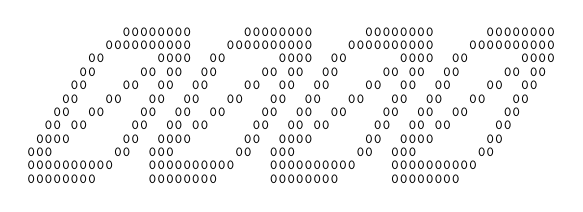
\begin{tikzpicture}[x=.11cm,y=.17cm]
\foreach \x/\y in {11/0,12/0,13/0,14/0,15/0,16/0,17/0,18/0,9/-1,10/-1,11/-1,12/-1,13/-1,14/-1,15/-1,16/-1,17/-1,18/-1,7/-2,8/-2,15/-2,16/-2,17/-2,18/-2,6/-3,7/-3,13/-3,14/-3,16/-3,17/-3,5/-4,6/-4,11/-4,12/-4,15/-4,16/-4,4/-5,5/-5,9/-5,10/-5,14/-5,15/-5,3/-6,4/-6,7/-6,8/-6,13/-6,14/-6,2/-7,3/-7,5/-7,6/-7,12/-7,13/-7,1/-8,2/-8,3/-8,4/-8,11/-8,12/-8,0/-9,1/-9,2/-9,10/-9,11/-9,0/-10,1/-10,2/-10,3/-10,4/-10,5/-10,6/-10,7/-10,8/-10,9/-10,0/-11,1/-11,2/-11,3/-11,4/-11,5/-11,6/-11,7/-11,25/0,26/0,27/0,28/0,29/0,30/0,31/0,32/0,23/-1,24/-1,25/-1,26/-1,27/-1,28/-1,29/-1,30/-1,31/-1,32/-1,21/-2,22/-2,29/-2,30/-2,31/-2,32/-2,20/-3,21/-3,27/-3,28/-3,30/-3,31/-3,19/-4,20/-4,25/-4,26/-4,29/-4,30/-4,18/-5,19/-5,23/-5,24/-5,28/-5,29/-5,17/-6,18/-6,21/-6,22/-6,27/-6,28/-6,16/-7,17/-7,19/-7,20/-7,26/-7,27/-7,15/-8,16/-8,17/-8,18/-8,25/-8,26/-8,14/-9,15/-9,16/-9,24/-9,25/-9,14/-10,15/-10,16/-10,17/-10,18/-10,19/-10,20/-10,21/-10,22/-10,23/-10,14/-11,15/-11,16/-11,17/-11,18/-11,19/-11,20/-11,21/-11,39/0,40/0,41/0,42/0,43/0,44/0,45/0,46/0,37/-1,38/-1,39/-1,40/-1,41/-1,42/-1,43/-1,44/-1,45/-1,46/-1,35/-2,36/-2,43/-2,44/-2,45/-2,46/-2,34/-3,35/-3,41/-3,42/-3,44/-3,45/-3,33/-4,34/-4,39/-4,40/-4,43/-4,44/-4,32/-5,33/-5,37/-5,38/-5,42/-5,43/-5,31/-6,32/-6,35/-6,36/-6,41/-6,42/-6,30/-7,31/-7,33/-7,34/-7,40/-7,41/-7,29/-8,30/-8,31/-8,32/-8,39/-8,40/-8,28/-9,29/-9,30/-9,38/-9,39/-9,28/-10,29/-10,30/-10,31/-10,32/-10,33/-10,34/-10,35/-10,36/-10,37/-10,28/-11,29/-11,30/-11,31/-11,32/-11,33/-11,34/-11,35/-11,53/0,54/0,55/0,56/0,57/0,58/0,59/0,60/0,51/-1,52/-1,53/-1,54/-1,55/-1,56/-1,57/-1,58/-1,59/-1,60/-1,49/-2,50/-2,57/-2,58/-2,59/-2,60/-2,48/-3,49/-3,55/-3,56/-3,58/-3,59/-3,47/-4,48/-4,53/-4,54/-4,57/-4,58/-4,46/-5,47/-5,51/-5,52/-5,56/-5,57/-5,45/-6,46/-6,49/-6,50/-6,55/-6,56/-6,44/-7,45/-7,47/-7,48/-7,54/-7,55/-7,43/-8,44/-8,45/-8,46/-8,53/-8,54/-8,42/-9,43/-9,44/-9,52/-9,53/-9,42/-10,43/-10,44/-10,45/-10,46/-10,47/-10,48/-10,49/-10,50/-10,51/-10,42/-11,43/-11,44/-11,45/-11,46/-11,47/-11,48/-11,49/-11}{\node[inner sep=0pt,font=\ttfamily\tiny] at (\x,\y) {0};}
\end{tikzpicture}%
}
\figure{%
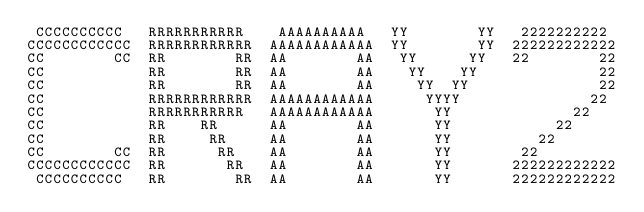
\begin{tikzpicture}[x=.11cm,y=.17cm]
\foreach \x/\y in {1/0,2/0,3/0,4/0,5/0,6/0,7/0,8/0,9/0,10/0,0/-1,1/-1,2/-1,3/-1,4/-1,5/-1,6/-1,7/-1,8/-1,9/-1,10/-1,11/-1,0/-2,1/-2,10/-2,11/-2,0/-3,1/-3,0/-4,1/-4,0/-5,1/-5,0/-6,1/-6,0/-7,1/-7,0/-8,1/-8,0/-9,1/-9,10/-9,11/-9,0/-10,1/-10,2/-10,3/-10,4/-10,5/-10,6/-10,7/-10,8/-10,9/-10,10/-10,11/-10,1/-11,2/-11,3/-11,4/-11,5/-11,6/-11,7/-11,8/-11,9/-11,10/-11}{\node[inner sep=0pt,font=\ttfamily\tiny] at (\x,\y) {C};}
\foreach \x/\y in {14/0,15/0,16/0,17/0,18/0,19/0,20/0,21/0,22/0,23/0,24/0,14/-1,15/-1,16/-1,17/-1,18/-1,19/-1,20/-1,21/-1,22/-1,23/-1,24/-1,25/-1,14/-2,15/-2,24/-2,25/-2,14/-3,15/-3,24/-3,25/-3,14/-4,15/-4,24/-4,25/-4,14/-5,15/-5,16/-5,17/-5,18/-5,19/-5,20/-5,21/-5,22/-5,23/-5,24/-5,25/-5,14/-6,15/-6,16/-6,17/-6,18/-6,19/-6,20/-6,21/-6,22/-6,23/-6,24/-6,14/-7,15/-7,20/-7,21/-7,14/-8,15/-8,21/-8,22/-8,14/-9,15/-9,22/-9,23/-9,14/-10,15/-10,23/-10,24/-10,14/-11,15/-11,24/-11,25/-11}{\node[inner sep=0pt,font=\ttfamily\tiny] at (\x,\y) {R};}
\foreach \x/\y in {29/0,30/0,31/0,32/0,33/0,34/0,35/0,36/0,37/0,38/0,28/-1,29/-1,30/-1,31/-1,32/-1,33/-1,34/-1,35/-1,36/-1,37/-1,38/-1,39/-1,28/-2,29/-2,38/-2,39/-2,28/-3,29/-3,38/-3,39/-3,28/-4,29/-4,38/-4,39/-4,28/-5,29/-5,30/-5,31/-5,32/-5,33/-5,34/-5,35/-5,36/-5,37/-5,38/-5,39/-5,28/-6,29/-6,30/-6,31/-6,32/-6,33/-6,34/-6,35/-6,36/-6,37/-6,38/-6,39/-6,28/-7,29/-7,38/-7,39/-7,28/-8,29/-8,38/-8,39/-8,28/-9,29/-9,38/-9,39/-9,28/-10,29/-10,38/-10,39/-10,28/-11,29/-11,38/-11,39/-11}{\node[inner sep=0pt,font=\ttfamily\tiny] at (\x,\y) {A};}
\foreach \x/\y in {42/0,43/0,52/0,53/0,42/-1,43/-1,52/-1,53/-1,43/-2,44/-2,51/-2,52/-2,44/-3,45/-3,50/-3,51/-3,45/-4,46/-4,49/-4,50/-4,46/-5,47/-5,48/-5,49/-5,47/-6,48/-6,47/-7,48/-7,47/-8,48/-8,47/-9,48/-9,47/-10,48/-10,47/-11,48/-11}{\node[inner sep=0pt,font=\ttfamily\tiny] at (\x,\y) {Y};}
\foreach \x/\y in {57/0,58/0,59/0,60/0,61/0,62/0,63/0,64/0,65/0,66/0,56/-1,57/-1,58/-1,59/-1,60/-1,61/-1,62/-1,63/-1,64/-1,65/-1,66/-1,67/-1,56/-2,57/-2,66/-2,67/-2,66/-3,67/-3,66/-4,67/-4,65/-5,66/-5,63/-6,64/-6,61/-7,62/-7,59/-8,60/-8,57/-9,58/-9,56/-10,57/-10,58/-10,59/-10,60/-10,61/-10,62/-10,63/-10,64/-10,65/-10,66/-10,67/-10,56/-11,57/-11,58/-11,59/-11,60/-11,61/-11,62/-11,63/-11,64/-11,65/-11,66/-11,67/-11}{\node[inner sep=0pt,font=\ttfamily\tiny] at (\x,\y) {2};}
\end{tikzpicture}%
}

\diagram{\begin{array}{lllllllllll}
\texttt{****A}&\texttt{END}&\texttt{JOB 352}&\texttt{CRAY2}&\texttt{ROOM}&\texttt{3.11.31 PM 19 AUG 82}&\texttt{R6.PR1}&\texttt{SYS JES2}&\texttt{JOB 352}&\texttt{END}&\texttt{A****}\\
\texttt{****A}&\texttt{END}&\texttt{JOB 352}&\texttt{CRAY2}&\texttt{ROOM}&\texttt{3.11.31 PM 19 AUG 82}&\texttt{R6.PR1}&\texttt{SYS JES2}&\texttt{JOB 352}&\texttt{END}&\texttt{A****}\\
\texttt{****A}&\texttt{END}&\texttt{JOB 352}&\texttt{CRAY2}&\texttt{ROOM}&\texttt{3.11.31 PM 19 AUG 82}&\texttt{R6.PR1}&\texttt{SYS JES2}&\texttt{JOB 352}&\texttt{END}&\texttt{A****}\\
\texttt{****A}&\texttt{END}&\texttt{JOB 352}&\texttt{CRAY2}&\texttt{ROOM}&\texttt{3.11.31 PM 19 AUG 82}&\texttt{R6.PR1}&\texttt{SYS JES2}&\texttt{JOB 352}&\texttt{END}&\texttt{A****}\\
\texttt{****A}&\texttt{END}&\texttt{JOB 352}&\texttt{CRAY2}&\texttt{ROOM}&\texttt{3.11.31 PM 19 AUG 82}&\texttt{R6.PR1}&\texttt{SYS JES2}&\texttt{JOB 352}&\texttt{END}&\texttt{A****}\\
\texttt{****A}&\texttt{END}&\texttt{JOB 352}&\texttt{CRAY2}&\texttt{ROOM}&\texttt{3.11.31 PM 19 AUG 82}&\texttt{R6.PR1}&\texttt{SYS JES2}&\texttt{JOB 352}&\texttt{END}&\texttt{A****}
\end{array}}

\scanpage{28}
\margin{27}

artificiels aux bord du disque, \unsure{sûrement rédhibitoires}, i.e. \unsure{certaines|certains} ps. droites de $\Delta(D)$, qui \unsure{se rencontraient} pas dans $\Delta(D)$, vont se rencontrer sur le bord de $\Delta'(D)$ \deleted{\unsure{;} }. Si on fait par contre les recollements \deleted{\unsure{sur}} \inserted{des} $\Delta(D)$, sans faire les identifications qui mènent aux $\Delta'(D)$, on trouve une \uline{surface à bord} (\inserted{bord} en vert), d'où à nouveau, en bouchant les trous \inserted{par des disques $\Delta_\alpha$}, une surface sans bord compacte. (On obtient la surface envisagée au début en contractant \inserted{chacun des} ces disques en \deleted{\unsure{des}} un point.) La surface cellulaire à bord obtenue est telle que les pts du bord sont \deleted{doubles ou triples} \inserted{tous d'ordre 2 ou trois}, et chaque sommet est sur le bord, elle se déduit de la carte sans bord par le procédé canonique, consistant à enlever un petit disque autour de chaque sommet. En tous cas, les trous à boucher dans la surface à bord correspondent exactement aux sommets de la surface sans bord.

\margin{\unsure{avec un grain de sel} $\nearrow$}

\uline{25.12}

Il faudrait regarder la \unsure{relation} entre $\operatorname{Pol}(D)$ et $\operatorname{Pol}(D')$, quand $D\longrightarrow D'$ et $D'$ supercritique. Il faudrait déjà \uline{définir} $\operatorname{Pol}(D')$, i.e. $\operatorname{Pol}(\Delta)$ quand $\Delta\in\Sigma$, comme l'une des \unsure{générisations} de $\Delta$, avec une structure polygonale convenable dessus. On a vu que les \deleted{\unsure{spécialisations}} \unsure{générisations} de $\Delta$ correspondent aux sommets sur $\widetilde\Delta$, image inverse de $\Delta$ dans $\widetilde X$. D'ailleurs pour un sommet $s$ de $\Delta$,

\figure{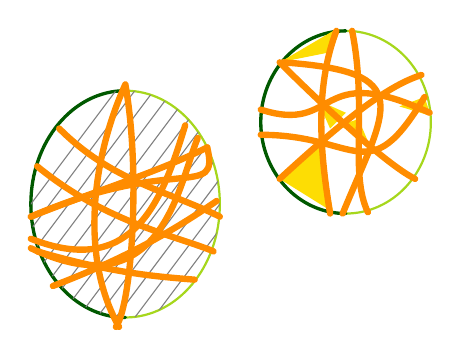
\begin{tikzpicture}[x=.8cm,y=.8cm,line cap=round,line join=round]
\begin{scope}[shift={(0,0)}]
\draw[yellow!65!green,thick] (0,0) ellipse(1.5 and 1.8);\draw[green!35!black,very thick] (90:1.5 and 1.8) arc(90:270:1.5 and 1.8);
\begin{scope}\clip (0,0) ellipse(1.5 and 1.8);\foreach \t in {-3,-2.7,...,2}{\draw[gray] (\t,-2)--({\t+3},2);}\end{scope}
\draw[orange!90!yellow,line width=2.3pt] (0,1.9)..controls(-.5,.8)and(-.75,-.8)..(-.1,-1.95) (0,1.9)..controls(.25,.5)and(.1,-1.6)..(-.15,-1.95);
\draw[orange!90!yellow,line width=2.3pt] (-1.05,1.2)..controls(-.2,.35)and(.7,.2)..(1.5,-.2) (-1.4,.6)..controls(-.3,-.3)and(.8,-.5)..(1.4,-.75);
\draw[orange!90!yellow,line width=2.3pt] (-1.5,-.2)..controls(-.5,.2)and(.5,.5)..(1.3,.9) (-1.5,-.55)..controls(.15,-1.2)and(.6,.1)..(.95,1.25);
\draw[orange!90!yellow,line width=2.3pt] (-1.5,-.7)..controls(.6,-1.7)and(.85,.35)..(1.15,1.05) (-1.15,-1.3)..controls(-.1,-.9)and(.65,-.5)..(1.45,.05);
\draw[orange!90!yellow,line width=2.3pt] (-1.4,-.75)..controls(-.2,-1.1)and(.5,-1.15)..(1.1,-1.2) (-1.5,-.2)..controls(.8,.8)and(1.5,.05)..(1.3,.9);
\end{scope}
\begin{scope}[shift={(3.5,1.3)}]
\draw[yellow!65!green,thick] (0,0) ellipse(1.35 and 1.45);\draw[green!35!black,very thick] (90:1.35 and 1.45) arc(90:270:1.35 and 1.45);
\fill[yellow!80!orange] (-1.05,.95)--(-.2,1.45)--(-.3,1.1)--cycle;
\fill[yellow!80!orange] (-1.05,-.9)--(-.42,-.3)--(-.2,-1.43)--cycle;
\fill[yellow!80!orange] (-.45,.35)--(-.25,-.1)--(0,.15)--cycle;
\fill[yellow!80!orange] (.2,.05)--(.35,-.3)--(-.1,-.05)--cycle;
\fill[yellow!80!orange] (1.25,.4)--(1.35,.1)--(.85,.25)--cycle;
\draw[orange!90!yellow,line width=2.3pt] (-.15,1.45)..controls(-.55,.4)and(-.35,-.8)..(-.25,-1.45) (.1,1.45)..controls(.35,.2)and(.05,-.8)..(.35,-1.43);
\draw[orange!90!yellow,line width=2.3pt] (-1.05,.95)..controls(-.2,.1)and(.7,-.7)..(1.1,-.9) (-1.35,.2)..controls(-.1,-.2)and(-.5,1)..(1.33,.15);
\draw[orange!90!yellow,line width=2.3pt] (-1.35,-.2)..controls(.2,-.2)and(.35,-1.1)..(1.25,.4) (-1.05,-.9)..controls(.2,.25)and(.75,.6)..(1.2,.75);
\draw[orange!90!yellow,line width=2.3pt] (-1,.95)..controls(1.15,.8)and(.65,.25)..(-.05,-1.45);
\end{scope}
\end{tikzpicture}}

\scanpage{29}
\margin{28}

les pts de $\widetilde\Delta$ au dessus de $s$ i.e. les orientations de $X$ en $s$, correspondent aux \inserted{deux} vis de $\Delta\setminus\{s\}$ dans $X$. La spécialisation $D\mathbin{-}D'$ définit une de ces vis (celle balayée par la spécialisation), et on trouve un isom. combinatoire canonique entre les segments combinatoires correspondants : la vis de spécialisation sur $D$, et celle correspondant à \inserted{l'intérieur de} la vis balayée de $D'\setminus\{s\}$, \inserted{i.e. le \uline{\unsure{découpage}} de $D'$ \unsure{suivant} $s$.} (En termes de $D'$, le choix d'un \deleted{point} \inserted{sommet} $\widetilde s$ de $\widetilde{D'}$, \uline{d'où} un antipodique $\widetilde s^-$, partage $\widetilde{D'}$ en deux arcs, correspondant aux deux orientations de $\widetilde{D'}$ en les considérant comme \deleted{les} deux arcs \uline{orientés} d'origine $\widetilde s$, extrémité $\widetilde s^-$).

\deleted{L'antipodisme de $\widetilde{D'}$ qui \unsure{échange les deux} \inserted{échange $\widetilde s,\widetilde s^-$} \unsure{soit l'identité ou}}

\deleted{\unsure{Il y a un unique autre} \deleted{\unsure{isom}} combinatoire \inserted{$\ne\mathrm{id}$} \unsure{qui identifie} ces deux arcs, et qui \deleted{\unsure{les deux arcs}} --- par cet isom, on peut identifier les deux arcs combinatoires obtenus, d'où un arc combinatoire canonique.}

L'antipodisme définit un isom canonique entre ces deux arcs, qui permet \inserted{donc} d'identifier combinatoirement, \inserted{\unsure{soit} $\unsure{\mathbb{I}|\mathrm{I}}(D',s)$} \unsure{ce} segment combinatoire. D'où ce qu'on peut dire, c'est qu'on a un isom combinatoire canonique
\diagram{\begin{tikzcd}[ampersand replacement=\&]
\begin{gathered}\text{Vis de spécialisation}\\\text{de $D$ utilisée}\end{gathered}\arrow[r,"\sim"]\&\unsure{\mathbb{I}|\mathrm{I}}(D',s)
\end{tikzcd}}

\scanpage{30}
\margin{29}
\figure{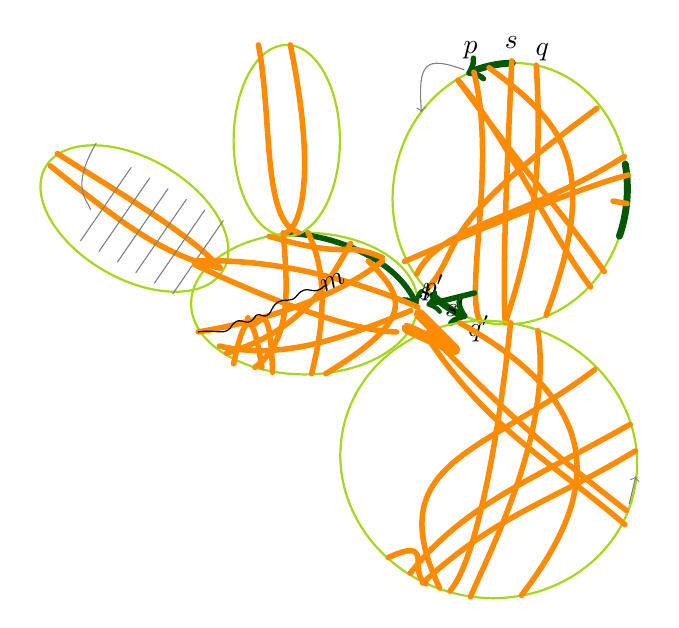
\begin{tikzpicture}[x=.9cm,y=.9cm,line cap=round,line join=round]
\draw[yellow!65!green,thick] (0,0) ellipse(1.6 and 1);
\draw[green!35!black,line width=2pt,->] (-.2,.99)..controls(.5,.95)and(1.3,.6)..(1.59,-.03);
\begin{scope}[shift={(-2.4,1.2)},rotate=-30]
\draw[yellow!65!green,thick] (0,0) ellipse(1.45 and .85);
\draw[orange!90!yellow,line width=2pt] (-1.4,.25)..controls(-.2,.2)and(.8,.2)..(1.4,0) (-1.4,.05)..controls(-.1,-.15)and(.6,-.25)..(1.4,0);
\foreach \x in {-.5,-.2,.1,.4,.7,1}{\draw[gray] (\x,-.65)--({\x+.1},.6);}
\draw[gray] (-1,.65)..controls(-1,-.1)and(-.7,-.1)..(-.6,-.2);
\end{scope}
\draw[yellow!65!green,thick] (-.25,2.3) ellipse(.75 and 1.35);
\draw[orange!90!yellow,line width=2pt] (-.65,3.65)..controls(-.45,2.6)and(-.6,1.15)..(-.08,1) (-.2,3.65)..controls(.1,2.2)and(.05,1.2)..(-.25,1);
\draw[orange!90!yellow,line width=2pt] (-1.55,.6)..controls(-.4,.65)and(.8,.3)..(1.6,-.05) (-1.55,.55)..controls(-.5,.05)and(.7,-.4)..(1.3,-.4);
\draw[orange!90!yellow,line width=2pt] (-.5,.95)..controls(.7,.6)and(.5,.9)..(1.1,.65) (-.3,1)..controls(-.25,.3)and(-.15,-.5)..(-.7,-.9) (.05,1)..controls(.4,.3)and(.2,-.6)..(.1,-.99);
\draw[orange!90!yellow,line width=2pt] (-1.5,-.4)..controls(-.3,-.2)and(.6,.2)..(1.1,.6) (-1.2,-.6)..controls(-.3,-.8)and(.5,-.5)..(1.5,-.1) (-1.1,-.7)..controls(-.1,-.4)and(.3,.2)..(.65,.85);
\draw[orange!90!yellow,line width=2pt] (-1,-.85)..controls(-.8,.1)and(-.7,-.3)..(-.6,-.9) (-.45,-.97)..controls(-.5,.4)and(-.7,-.6)..(-.8,-.2) (.3,-.99)..controls(1.6,-.2)and(1.4,.1)..(.9,.6);
\draw[black,line width=.45pt] (-1.5,-.4)..controls(-1.25,-.36)and(-1.15,-.45)..(-1.05,-.35)..controls(-.92,-.12)and(-.84,-.35)..(-.72,-.22)..controls(-.64,-.05)and(-.56,-.3)..(-.46,-.08)..controls(-.35,.14)and(-.19,-.03)..(-.1,.12)..controls(.05,.3)and(.12,.08)..(.28,.25);
\node[rotate=25] at(.4,.3){$\unsure{m}$};
\begin{scope}[shift={(2.9,1.55)},rotate=-10]
\draw[yellow!65!green,thick] (0,0) ellipse(1.65 and 1.85);
\draw[green!35!black,line width=2.5pt,->] (100:1.65 and 1.85) arc(100:123:1.65 and 1.85);
\draw[green!35!black,line width=2.5pt] (-10:1.65 and 1.85) arc(-10:22:1.65 and 1.85);
\draw[green!35!black,line width=2.5pt,->] (-120:1.65 and 1.85) arc(-120:-100:1.65 and 1.85);
\draw[orange!90!yellow,line width=2pt] (-.8,1.6)..controls(-.25,.4)and(-.4,-1.5)..(-.1,-1.85) (-.3,1.85)..controls(-.1,.3)and(.1,-1.2)..(.25,-1.8) (.05,1.85)..controls(.45,.2)and(.4,-.8)..(.25,-1.8);
\draw[orange!90!yellow,line width=2pt] (-1,1.45)..controls(-.2,.8)and(.6,-.4)..(1.35,-1.1) (-.6,1.7)..controls(.6,1.1)and(1.2,.6)..(.8,-1.6);
\draw[orange!90!yellow,line width=2pt] (-1.1,-1.35)..controls(-.9,-.6)and(.3,-.3)..(1.5,.8) (-1.3,-1.2)..controls(-1,-1)and(1,.3)..(1.6,.55) (-.9,-1.5)..controls(-.5,-.8)and(-1,-.7)..(1,1.4);
\draw[orange!90!yellow,line width=2pt] (-1,1.45)..controls(.3,.2)and(.8,-.15)..(1.5,-.85);
\draw[orange!90!yellow,line width=2pt] (1.45,.15)--(1.65,.15);
\node at(-.9,1.9){$p$};\node at(-.35,2.1){$\unsure{s}$};\node at(.1,2.05){$q$};
\node at(-.83,-1.5){$\unsure{p'}$};\node at(-.48,-1.7){$\unsure{s'}$};\node at(-.1,-1.95){$\unsure{q'}$};
\end{scope}
\begin{scope}[shift={(2.6,-2.2)},rotate=-12]
\draw[yellow!65!green,thick] (0,0) ellipse(2.1 and 1.95);
\draw[orange!90!yellow,line width=2pt] (-.1,1.95)..controls(.05,.6)and(.15,-1.4)..(-.15,-1.93) (.3,1.92)..controls(.8,.6)and(.3,-1.2)..(.15,-1.95);
\draw[orange!90!yellow,line width=2pt] (-1.2,1.58)..controls(-.1,.8)and(.8,.3)..(2.05,-.3) (-1.25,1.55)..controls(-.1,.4)and(.9,.15)..(2.07,-.5);
\draw[orange!90!yellow,line width=2pt] (-.8,1.8)..controls(1.65,1.05)and(1.55,-.3)..(.85,-1.78);
\draw[orange!90!yellow,line width=2pt] (-1.1,-1.65)..controls(-.5,-1.2)and(-.8,-1.8)..(-.5,-1.9) (-.75,-1.8)..controls(-.2,-.7)and(.6,-.2)..(1.85,.9) (-.55,-1.9)..controls(.3,-.7)and(1,-.4)..(2, .55) (-.3,-1.92)..controls(-1.5,-.35)and(-.1,.05)..(1.2,1.55);
\draw[gray,->] (2.07,-.2)--(2.08,.2);
\end{scope}
\draw[orange!90!yellow,line width=4pt] (1.62,-.15)--(2.12,-.65) (1.45,-.35)--(2.1,-.65);
\draw[green!35!black,line width=2pt,->] (2.4,.15)--(1.72,-.02);
\node at(1.7,.14){$\unsure{s}$};
\draw[gray,->] (2.25,3.3)..controls(1.7,3.5)and(1.6,3.4)..(1.65,2.7);
\end{tikzpicture}}

\diagram{\begin{array}{rll}
\texttt{1}&\texttt{//CRAY2\quad JOB\quad '\unsure{*********|**********},\qquad ',',\qquad ',}&\texttt{JOB 0352}\\
&\texttt{// MSGLEVEL=(1,1),MSGCLASS=A}&\\
\texttt{2}&\texttt{// EXEC CSSBATCH}&\\
\texttt{3}&\texttt{XXCSSBATCH PROC REG=100K,P=''}&\texttt{00010000}\\
\texttt{4}&\texttt{XXCSSBATCH EXEC PGM=CRBATCH,REGION=\&REG,PARM=\&P}&\texttt{00020000}\\
\texttt{5}&\texttt{XXSTEPLIB DD DSN=CISI.PROD.CSSBATCH.V1.YY01,DISP=SHR}&\texttt{00030003}\\
\texttt{6}&\texttt{XXSYSUT1 DD DSN=\&\&SYSUT1,UNIT=\unsure{SYSTSO|SYSTS0},SPACE=(TRK,30),DISP=(NEW,DELETE)}&\texttt{00031006}\\
\texttt{7}&\texttt{XXSYSUDUMP DD SYSOUT=*}&\texttt{00040000}\\
\texttt{8}&\texttt{XXCRJIF DD DSN=SYS1.CR.JIF,DISP=SHR}&\texttt{00050000}\\
\texttt{9}&\texttt{XXSYSIN DD DDNAME=CRAYIN}&\texttt{00060000}\\
\texttt{10}&\texttt{//CRAYIN DD *}&
\end{array}}

\scanpage{31}
\margin{30}

Considérons un graphe comb. $\Gamma=(S,\vec A,\sigma_0,\unsure{\alpha})$ avec une semi-circularisation (structure polygonale \inserted{donnée} sur l'ens des sommets issus d'une \unsure{arête} donnée) et \deleted{pour tout} d'isom de transport
\[
\varphi_{\vec a}:\underbrace{\omega(\vec A_s)}_{\omega_s}\mathbin{-}\underbrace{\omega(\vec A_t)}_{\omega_t}\qquad\text{pour }\vec a:s\longrightarrow t
\]
(satisfaisant la seule condition
\[
\varphi_{-\vec a}=\varphi_{\vec a}^{-1}
\]
)

On suppose pour simplifier que les ordres des sommets sont $\ge3$ (sinon il faut se donner, pour les sommets d'ordre $1\le\nu\le2$, une structure de polygône combinatoire ayant $\vec A_s$ comme ens des sommets, i.e. avec un ens de deux orientations, de façon à pouvoir \unsure{en tenir} à la donnée des $\varphi_{\vec a}$). La surface associée aux $\varphi_{\vec a}$ est obtenue ainsi : on considère la réalisation topologique canonique \inserted{par disque polygonal} du polygône dual de chaque $\vec A_s$ (ce qui peut se faire via une décomposition barycentrique de $\overline A_s$, qui donne une réalisation simultanée pour \deleted{les deux} $\overline A_s$ et pour le polygône dual, chaque réalisation $\operatorname{Dis}_s$ apparaissant comme réunion de $2\nu_s$ \uline{drapeaux} correspondant aux repères de $\vec A_s$ --- i.e. les arêtes de ces polygônes correspondent aux \deleted{faces} \inserted{sommets} de $\vec A_s$, i.e. aux arêtes \deleted{\unsure{de}} de $\Gamma$ \deleted{\unsure{d'}} d'origine $s$.

\margin{cas $\nu_s=1,2$ n'est pas exclu}

\figure{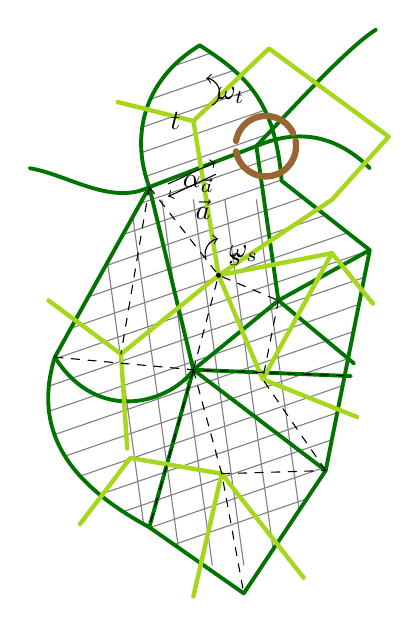
\begin{tikzpicture}[x=.8cm,y=.8cm,line cap=round,line join=round]
\begin{scope}\clip (-2,-.7)..controls(-2.4,-2)and(-1.6,-2.8)..(-.5,-3.4)--(1,-4.45)--(2.3,-2.5)--(3,1)--(1.6,2.1)..controls(1.5,3.4)and(1,3.8)..(.3,4.25)..controls(-.6,3.7)and(-.8,2.8)..(-.5,2)--cycle;
\foreach \y in {-4.5,-4.1,...,4}{\draw[gray] (-2.5,\y)--(3.3,{\y+2});}\foreach \x in {-.5,0,.5,1,1.5,2}{\draw[gray] (\x,-4)--({\x-.8},1.8);}\end{scope}
\draw[green!45!black,line width=1.4pt] (-2,-.7)..controls(-2.4,-2)and(-1.6,-2.8)..(-.5,-3.4)--(1,-4.45)--(2.3,-2.5)--(3,1)--(1.6,2.1)..controls(1.5,3.4)and(1,3.8)..(.3,4.25)..controls(-.6,3.7)and(-.8,2.8)..(-.5,2)--cycle;
\draw[green!45!black,line width=1.4pt] (-2,-.7)..controls(-1.3,-1.8)and(-.15,-1.4)..(.2,-.9)--(1.55,.2)--(3,1);
\draw[green!45!black,line width=1.4pt] (-.5,-3.4)--(.2,-.9)--(-.5,2)--(1.2,2.65)..controls(2,3)and(2.6,2.7)..(3,2.3);
\draw[green!45!black,line width=1.4pt] (.2,-.9)--(2.3,-2.5) (.2,-.9)--(2.7,-1) (1.2,2.65)--(1.55,.2)--(2.75,-.8);
\draw[green!45!black,line width=1.4pt] (1.2,2.65)..controls(2,3.5)and(2.7,4.25)..(3.1,4.5) (-.5,2)..controls(-1.1,1.7)and(-1.8,2.2)..(-2.4,2.3);
\draw[yellow!65!green,line width=1.6pt] (-1.6,-3.35)--(-.8,-2.3)--(.65,-2.55)--(1.95,-4.2) (.65,-2.55)--(.2,-4.5);
\draw[yellow!65!green,line width=1.6pt] (-2.1,.2)--(-.95,-.65)--(-.85,-2.15) (-.95,-.65)--(.6,.6)--(2.4,.95)--(3.05,.15);
\draw[yellow!65!green,line width=1.6pt] (-1,3.35)--(.2,3.05)--(.6,.6)--(1.3,-1.05)--(2.4,.95) (1.3,-1.05)--(2.8,-1.65);
\draw[yellow!65!green,line width=1.6pt] (.2,3.05)--(1.4,4.2)--(3.3,2.8)--(2.4,1.8)--(.6,.6);
\draw[dashed] (-2,-.7)--(.2,-.9)--(2.7,-1) (-.5,2)--(.6,.6)--(1.55,.2) (-.5,2)--(-.95,-.65) (.2,-.9)--(.6,.6) (.2,-.9)--(-.5,-3.4) (.2,-.9)--(.65,-2.55)--(1,-4.45) (.65,-2.55)--(2.3,-2.5) (1.55,.2)--(1.3,-1.05)--(2.3,-2.5);
\draw[brown!80!black,line width=2.3pt] (1.35,2.65) ++(10:.48) arc(10:-170:.48);\draw[brown!80!black,line width=2.3pt] (1.35,2.65) ++(25:.48) arc(25:170:.48);
\fill (.6,.6) circle(.04);\node[above right]at(.6,.6){$s$};\node[left]at(.15,3.05){$t$};
\draw[->] (.4,.85) arc(200:100:.25);\node at(1,.95){$\omega_s$};\draw[->] (.5,3.3) arc(-60:85:.23);\node at(.8,3.45){$\omega_t$};
\draw[->] (-.2,2.05)--(.55,2.4);\draw[<-] (-.2,1.85)--(.55,2.2);\node at(.35,1.65){$\vec a$};\node at(.28,2.05){$\unsure{\alpha_{\vec a}}$};
\end{tikzpicture}}

Ceci dit, on \uline{recolle}, pour tte $\vec a\in\vec A$ \deleted{$\unsure{\sigma_0}$}, posant $s=\operatorname{or}(\vec a)$, $t=\operatorname{ex}(\vec a)=\operatorname{or}(\unsure{\sigma\vec a|\alpha\vec a})$, \deleted{l'arête de $\operatorname{Dis}_s$} l'arête $\alpha_{\vec a}$ de $\operatorname{Dis}_s$ correspondant à $\vec a$, avec l'arête $\alpha_{-\vec a}$ de $\operatorname{Dis}_t$ correspondant à $-\vec a$, moyennant un isom \deleted{linéaire} \inserted{affine} sur les arêtes (donc défini \deleted{\unsure{par le choix}} d'une bijection sur les ens d'extrémités) \deleted{\unsure{avec le choix qui est donné}} \inserted{dont le choix est déterminé} à l'aide de l'isom de transport $\varphi_{\vec a}$ : la vérité, c'est que si les orientations $\omega_s$ de \deleted{$\operatorname{Dis}_s$} $\unsure{\vec A_s|\overline A_s}$, i.e. de $\operatorname{Dis}_s$, et $\omega_t$ de $\unsure{\vec A_t|\overline A_t}$, i.e. de $\operatorname{Dis}_t$, se correspondent, alors l'isom d'identification
\[
\psi_{\vec a}:\alpha_{\vec a}\xrightarrow{\sim}\alpha_{-\vec a}
\]
doit \deleted{\unsure{préserver}} \uline{renverser} les orientations induites par $\omega_s$ sur $\alpha_{\vec a}$ resp. $\omega_t$ sur $\alpha_{-\vec a}$.

\scanpage{32}
\margin{31}

Par ces identifications, on trouve une surface topologique \inserted{(\unsure{compacte sans bords})}, dans laquelle la réalisation topologique de $|\Gamma|$ de $\Gamma$ est canoniquement plongée. Les faces orientées de cette surface se réalisent comme les orbites sous l'opération $\rho_f$ sur l'ens \deleted{$\unsure{\vec A}$} $\operatorname{Rep}$ des couples $(\vec a,\omega)$, où $\vec a\in\vec A$, $\omega\in\underline\omega_s\overset{\mathrm{def}}=\underline\omega(\vec A_s)$, opération définie par
\[
\deleted{\rho_f(\vec a,\unsure{\omega})=}
\qquad\text{où }\boxed{\omega_t=\varphi_{\vec a}\omega_s\in\underline\omega(\unsure{A_s|A_t})}
\]
\[
\left\{\begin{aligned}
\rho_f(\vec a,\omega_s)&=(\vec b,\deleted{\unsure{\varphi_{\vec a}\omega_s}}\inserted{\omega_t})\\
\vec b&=\rho_{\omega_t}^{-1}(\deleted{\unsure{\sigma}}-\vec a)
\end{aligned}\right.
\qquad\begin{gathered}\text{et où }b\in\vec A_t\\(t=\operatorname{ex}(\vec a))\\\text{est donné par}\end{gathered}
\]
où $\rho_{\omega_t}$ est la permutation circulaire sur $\vec A_t$ définie par l'orientation $\omega_t$. C'est aussi l'opération de rotation autour des sommets de la carte duale $C^*$, définie par les faces en question.

Si on veut une description combinatoire complète de la carte $C$ définie par $(\Gamma,(\unsure{\pi_s})_{s\in S},(\varphi_{\vec a})_{\vec a\in\vec A})$, il faut expliciter les opérations $\sigma_0,\sigma_1,\sigma_2$ sur $\operatorname{Rep}C$, ens. des repères. On trouve
\margin{str. pol. sur $\vec A_s$}
\[
\left\{\begin{aligned}
\sigma_0(\vec a,\omega_s)&=(-\vec a,-\varphi_{\vec a}\omega_s)\\
\sigma_2(\vec a,\omega_s)&=(\vec a,-\omega_s)\\
\sigma_1(\vec a,\omega_s)&=(\deleted{\unsure{\vec a}}\rho_{\omega_s}(a),-\omega_s)
\end{aligned}\right.
\]
\figure{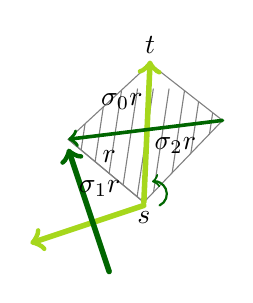
\begin{tikzpicture}[x=.8cm,y=.8cm,line cap=round]
\draw[gray] (0,0)--(-1.2,1)--(.1,2.2)--(1.25,1.3)--cycle;
\draw[gray] (-1.2,1)--(1.25,1.3) (-1.2,1)--(0,0);
\begin{scope}\clip(0,0)--(-1.2,1)--(.1,2.2)--(1.25,1.3)--cycle;\foreach\x in {-1.4,-1.15,...,1.2}{\draw[gray](\x,-.2)--({\x+.3},1.8);}\end{scope}
\draw[yellow!65!green,line width=2pt,->] (0,0)--(.1,2.25);\draw[yellow!65!green,line width=2pt,->] (0,-.05)--(-1.8,-.65);
\draw[green!40!black,line width=2pt,->] (-.55,-1.1)--(-1.2,.85);\draw[green!40!black,line width=1.3pt,->](1.25,1.3)--(-1.2,1);
\draw[green!40!black,thick,->](.25,-.05)arc(-65:100:.2);
\node[below]at(0,0){$s$};\node[above]at(.1,2.2){$t$};\node at(-.55,.72){$r$};\node at(-.35,1.6){$\sigma_0r$};\node at(.5,.9){$\sigma_2r$};\node at(-.7,.22){$\unsure{\sigma_1r}$};
\end{tikzpicture}}

Soit encore, en termes de repères $r$ des $\vec A_s$, en interprétant
\[
\operatorname{Rep}(C)\simeq\coprod_{s\in S}\underbrace{\operatorname{Rep}(\vec A_s)}_{\text{ens des drapeaux}}
\]
\margin{\deleted{\unsure{par le côté}} $\vec a$.}
\[
\left\{\begin{aligned}
\sigma_0(r)&=\deleted{\unsure{(\vec a,\omega)\text{ repère de l'arête}}}\ r',\quad\text{défini par }\left\{\begin{aligned}\unsure{ar_{r'}|a_{r'}}&=-\vec a\\\omega_{r'}&=-\varphi_{\vec a}\omega_r)\end{aligned}\right.\\
\sigma_1(r)&=\widetilde\sigma_0(r)\\
\sigma_2(r)&=\widetilde\sigma_1(r)
\end{aligned}\right.
\]
où $\widetilde\sigma_0^s,\widetilde\sigma_1^s$ sont les opérations sur $\operatorname{Rep}(\vec A_s)$ habituelles, $\widetilde\sigma_i^s$ changeant le composant \inserted{du drapeau} de dimension $i$, pas l'autre.

En termes de ces opérations, on trouve
\[
\left\{\begin{aligned}
\rho_{\mathrm{som}}&=\sigma_2\sigma_{\unsure{1|4}}\deleted{\unsure{\xi}}=\widetilde\sigma_0^s\widetilde\sigma_1^s=\widetilde\rho^s\\
\rho_{\mathrm{face}}&=\sigma_1\sigma_0
\end{aligned}\right.
\]
\inserted{sur $\operatorname{Rep}_s=\operatorname{Rep}(\vec A_s)$}
\margin{opération de rotation \unsure{sur l'ens} des rep. d'un polygone comb.)}
Donc
\[
\rho_{\mathrm{som}}\rho_f=\sigma_2\sigma_0\overset{\mathrm{def}}=\sigma
\qquad\sigma(\vec a,\omega_s)=(-\vec a,\varphi_{\vec a}(\omega_s)).
\]

\scanpage{33}
\margin{32}

La subdivision barycentrique de $C$, qui est aussi celle de $C^*$, est apparente sur la description donnée, ses faces sont les drapeaux qui ont servi de composants pour la construction des $\operatorname{Dis}_s=|\vec A_s|$. (Cf traits \figure{\begin{tikzpicture}[baseline=-.5ex]\draw[green!40!black,thick](0,0)--(.6,0);\draw[yellow!65!green,thick](.8,0)--(1.4,0);\draw[dashed](1.6,0)--(2.2,0);\end{tikzpicture}})

On va donner une autre construction, de la surface $\mathcal X$ sous-jacente à $C$, qui s'obtient intuitivement en \unsure{traçant|tirant} des petits disques \deleted{\unsure{les}} autour des sommets de la \deleted{face} \inserted{carte} duale, \inserted{(centres des faces de $C$)} et \unsure{enlevant|incluant} les portions d'arêtes de $C^*$ (bleues) qui se trouvent à l'intérieur. La \uline{surface à bord} déduite de $\unsure{C^a|C^*}$ en enlevant les disques, avec la décomposition cellulaire définie par la construction précédente (dont les faces de $\unsure{C'}$ étant \unsure{réalisées|représentées} par les $\operatorname{Dis}_s$ ($s\in S$)), s'obtient en remplaçant les $\operatorname{Dis}_s$ par les $\operatorname{Dis}'_s$, obtenus en ``enlevant les coins'' de ces plaques polygonales. Chaque $\vec A_s$ est remplacé par le polygone combinatoire ``doublé'' $\unsure{\vec A'_s}$ (\deleted{\unsure{l'ens des sommets}} \inserted{dont les \deleted{sommets} arêtes sont les} repères de $\vec A_s$), \deleted{dont le} d'ordre $\unsure{2\nu}$, et en prenant le polygone dual, dont les ``arêtes'' \inserted{\unsure{d'inertie}} sont en corr. biunivoque avec les \deleted{repères} \inserted{arêtes de $\vec A_s$} \deleted{de $\vec A_s$}, et les ``arêtes de recollement'' avec les \deleted{\unsure{qui sont les repères, c'est les sommets}} \inserted{sommets de $\vec A_s$} \deleted{\unsure{qui sont}}. Ceci dit, en recollant les $\operatorname{Dis}_s$ ($s\in S$) suivant les arêtes de recollement seulement, on trouve une carte à bord dont les faces sont les $\operatorname{Dis}'_s$, et les comp. connexes du bord sont en corr. $1-1$ avec l'ens des faces de $C$ i.e. les sommets de $C^*$ --- donc ce sont les orbites sous le groupe diédral $\langle\sigma_1,\sigma_0\rangle$ contenant $\langle\rho_f\rangle$ comme un sous-groupe d'indice (1 ou) 2. Notons que dans le procédé de recollement précédent, chaque composante connexe \deleted{\unsure{d'inertie|d'intérieur}} du bord apparaît comme un polygone topologique, \unsure{d'indice égal à l'ordre|l'indice égale l'ordre}

\figure{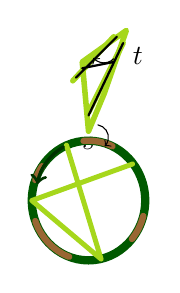
\begin{tikzpicture}[x=.8cm,y=.8cm,line cap=round,line join=round]
\draw[yellow!65!green,line width=2pt] (0,1.1)--(-.1,2.2)--(.6,2.7)--(.25,1.7)--cycle;
\draw[yellow!65!green,line width=2pt] (-.25,1.9)--(.4,2.6) (0,1.4)--(.55,2.5);
\draw[black,thick] (-.2,1.95)--(.45,2.6) (0,1.35)--(.55,2.5) (-.1,2.1)--(.4,2.2);
\draw[black,->] (.4,2.25)arc(-45:-140:.22);\node[right]at(.55,2.3){$t$};\node[below]at(0,1.15){$s$};
\draw[green!35!black,line width=3pt] (0,0) ellipse(.9 and .95);
\draw[yellow!65!green,line width=1.8pt] (-.35,.88)--(.2,-.93) (-.9,0)--(.7,.58) (-.9,0)--(.2,-.93);
\draw[brown!80!black,line width=2.3pt] (65:.9 and .95)arc(65:95:.9 and .95) (145:.9 and .95)arc(145:160:.9 and .95) (200:.9 and .95)arc(200:250:.9 and .95) (-15:.9 and .95)arc(-15:-40:.9 and .95);
\draw[green!20!black,very thick,->] (-.4,.85)arc(120:170:.85);\draw[black,->] (.15,1.2)arc(80:-45:.2);
\end{tikzpicture}}

\diagram{\begin{array}{lllll}
\texttt{PAGE 1}&\texttt{ON=CELMPQRSTV}&\texttt{08/19/82-15:06:51}&\texttt{CFT 1.09(06/28/82)}&\texttt{PAGE 1}
\end{array}}
\diagram{\begin{array}{rrl}
\texttt{1}&\texttt{1.}&\texttt{PROGRAM CRAY7}\\
\texttt{2}&\texttt{2.}&\texttt{WRITE(6,1)}\\
\texttt{3}&\texttt{3.}&\texttt{1 FORMAT(' BONJOUR')}\\
\texttt{4}&\texttt{4.}&\texttt{STOP}\\
\texttt{5}&\texttt{5.}&\texttt{END}
\end{array}}

\scanpage{34}
\margin{33}
du sommet correspondant de $C^*$. De façon plus précise, les côtés correspondent biunivoquement aux \uline{arêtes} du polygone local des arêtes \deleted{de} issues de $\unsure{\sigma|s}$, ou encore aux sommets de $\Gamma$ incidents à la face.

Plus précisément encore, le polygône comb. associé à cette comp. connexe du bord est can. isom. au \uline{dual} du polygône combinatoire correspondant à la face envisagée de $C$. \unsure{(}

Dans le cas qui nous intéresse, provenant d'un syst. de ps. droites $\Sigma$, en prenant la carte \unsure{structurelle} de toutes les positions relatives, il se trouve que l'ordre de toutes ces faces est (un diviseur de) 4. De plus, parmi les \inserted{quatre} côtés des diverses comp. connexes du bord, correspondant donc à un \uline{coin} de la carte $C$, il y en a un qui est \uline{privilégié}

Mais la propriété de ``type'' qui le distingue ne dépend pas \inserted{(en général)} que du sommet correspondant de $C$ \inserted{i.e. de $\Gamma$}, mais bien du coin \deleted{\unsure{qui la}} particulier envisagé. Donc il n'y a \deleted{\unsure{pas}} guère d'espoir, en général, de réaliser \inserted{le graphe sous-jacent à} $C$ comme réunion de deux \deleted{cartes $C_0,C$} graphes $\gamma,\gamma^*$, correspondants topologiquement à deux \deleted{\unsure{graphes d}} \inserted{cartes} \unsure{duales} sur $\mathcal X$, duales l'une de l'autre.

Soit $\underline\Sigma=(X,\Sigma)$ un syst. de pseudo-droites, et $L\deleted{D}$ une position relative (non triviale). On prend une \deleted{petite}\inserted{étroite} bande \inserted{(de Möbius) $\beta_L$} autour de $L$, dont le bord $\widetilde L$ peut être vu comme rev. à deux feuillets de $\unsure{L|D}$ (\uline{\unsure{rev.|rec.} des vis}), et le complémentaire de $\mathring\beta_L$ est un disque, \deleted{$\unsure{D_L=\Delta_L}$} soit $\Delta_L$. Toute $D_i\in\Sigma$ coupe $\partial\Delta_L=\deleted{\unsure{D}}\widetilde L$ \deleted{\unsure{sur}} en exactement deux points, et sa trace sur \deleted{$\unsure{D_{\Delta_L}}$} sur $\Delta_L$ est un segment (ainsi que sa trace dans $\beta_L$).

\scanpage{35}
\margin{34}
\figure{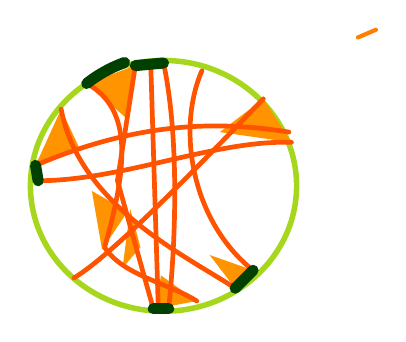
\begin{tikzpicture}[x=.65cm,y=.65cm,line cap=round,line join=round]
\draw[yellow!65!green,line width=2pt] (0,0) ellipse (2.6 and 2.45);
\fill[orange!85!yellow] (-1.5,2)--(-.7,1.3)--(-.55,2.35)--cycle;
\fill[orange!85!yellow] (-2.5,.4)--(-1.65,.75)--(-2,1.5)--cycle;
\fill[orange!85!yellow] (1.95,1.7)--(1.1,1.05)--(2.5,.85)--cycle;
\fill[orange!85!yellow] (-1.4,-.1)--(-.7,-.5)--(-1.2,-1.25)--cycle;
\fill[orange!85!yellow] (-.65,-.45)--(-.45,-1.2)--(-.8,-1.6)--cycle;
\fill[orange!85!yellow] (.65,-2.25)--(-.05,-1.75)--(-.15,-2.4)--cycle;
\fill[orange!85!yellow] (1.4,-2)--(.9,-1.35)--(1.75,-1.65)--cycle;
\draw[orange!65!red,line width=1.7pt] (-1.5,2) .. controls (-.6,1.5) and (-.7,.4) .. (-1.15,-1.2) .. controls (-.8,-1.75) and (.1,-1.9) .. (.65,-2.25);
\draw[orange!65!red,line width=1.7pt] (-.55,2.35)--(-.9,.1)--(-.2,-2.4);
\draw[orange!65!red,line width=1.7pt] (-.25,2.4)--(-.1,-2.45);
\draw[orange!65!red,line width=1.7pt] (0,2.4) .. controls (.3,1) and (.25,-1) .. (.1,-2.4);
\draw[orange!65!red,line width=1.7pt] (.75,2.25) .. controls (.25,1.1) and (.55,-.7) .. (1.75,-1.65);
\draw[orange!65!red,line width=1.7pt] (1.95,1.7) .. controls (.75,.45) and (-1,-1.35) .. (-1.75,-1.8);
\draw[orange!65!red,line width=1.7pt] (-2.45,.1) .. controls (-.8,.1) and (1,.9) .. (2.5,.85);
\draw[orange!65!red,line width=1.7pt] (-2.5,.4) .. controls (-.4,1.3) and (1.2,1.25) .. (2.45,1.05);
\draw[orange!65!red,line width=1.7pt] (-2,1.5) .. controls (-1.65,-.4) and (.5,-1.4) .. (1.4,-2);
\draw[green!25!black,line width=4pt] (-1.5,2) arc (130:111:2.6 and 2.45);
\draw[green!25!black,line width=4pt] (-.55,2.35)--(0,2.4);
\draw[green!25!black,line width=4pt] (-2.5,.4)--(-2.45,.1);
\draw[green!25!black,line width=4pt] (-.2,-2.4)--(.1,-2.4);
\draw[green!25!black,line width=4pt] (1.4,-2)--(1.75,-1.65);
\draw[orange,line width=1.5pt] (3.8,2.9)--(4.15,3.05);
\end{tikzpicture}}
On trouve un ``syst. de cordes'' \inserted{$d_i=(D_i)_L$} dans $\Delta=\Delta_L$ qui a les propriétés suivantes

a) Deux $d_i$ se coupent en au plus un point, lequel est \uline{intérieur} à $\Delta$, et elles se croisent en ce point.

(Cela fait partie de la notion $:=$ de ``syst de cordes'', \inserted{\unsure{déf°}} avec la condition que les $d_i$ soient des segments topologiques et $\partial d_i=d_i\cap\partial\Delta$)

b) La relation dans $I$ ``$i=j$ ou \deleted{$\unsure{d_i\ne d_j}$} $\delta_i\cap\delta_j=\varnothing$'' \deleted{est} (``parallélisme'') est une relation d'équivalence, et \deleted{\unsure{si l'on}} si on a une classe \deleted{\unsure{d'équivalence de $\nu$ éléments}} \inserted{d'équi. $C$, \deleted{\unsure{qui a plus}} $\nu\geq2$}, alors l'ensemble des \inserted{$2\nu$} sommets correspondants est réparti en 2 paquets \inserted{$S',S''$} de $\nu$, \deleted{\unsure{un}} [naturellement \inserted{\unsure{non-}}antipodiques] (NB cela a un sens rigoureusement combinatoire, les \unsure{bds $\partial\delta$} des segments du syst. étant une \unsure{paire})] \inserted{avec \deleted{\unsure{les}} $\delta\cap S'$ et $\delta\cap S''$ réduits à un point pour t\textsuperscript{t} $\delta\in C$}, et les sommets des ch. des deux paquets, forment vis à vis de $C$ fixe, $(s_1,s_2,\ldots,s_\nu)$ avec deux sommets consécutifs adjacents. [Cette partition de l'ens. \deleted{\unsure{des}} des $2\nu$ sommets est unique.]
\margin{[ ] est supprimé}

Ces conditions combinatoires nécessaires pour que le syst. de cordes soit isomorphe à celui d'une position relative p.r. à un $\Sigma$ convenable, est aussi suffisante. Elles impliquent que si on choisit un représentant dans chaque classe de parallélisme on trouve un syst. de cordes strict (i.e. \unsure{tot.\textsuperscript{t} par-ordré}).

Pour $C$ donné, considérons les arcs topologiques interceptés par les ensembles $S',S''$ on trouve deux arcs (topologiques, ou combinatoires), appelés \uline{arcs de générisation} relatifs à $L$ (et à $C$). L'ens. de tous ces arcs, que $L$ oscille. (marqués en bleu), \inserted{divisé par l'antipodisme,} est en corr. biunivoque avec l'ensemble $L\cap S$ ($S=S(\Sigma)$). \deleted{En}

On définit de plus les \uline{arcs de spécialisation}, en considérant les triangles formés par le système de cordes, adjacents à $\partial\Delta$. On considère les ensembles de sommets

\scanpage{36}
\margin{35}
$\sigma$ ayant les propriétés suivantes \inserted{$\operatorname{card}\sigma\geq2$, et}

a) \deleted{il existe un} \inserted{$\sigma$} forme un arc combinatoire sur l'ens. des sommets du syst. de cordes.

b) Les $D_{i(s)}$ passant par les $s\in\sigma$ sont mutuellement \unsure{disjoints|distincts}, et passent par un même sommet (\unsure{bien sûr unique}) $\deleted{\unsure{a}}\inserted{t}$, et toute \deleted{droite}\inserted{corde} passant par $t$ est parmi les $D_{i(s)}$.

c) \deleted{Tout} Les $s\in\sigma$, (ce qui revient au $=$, \deleted{\unsure{l'enveloppe du petit triangle intercepté}}, les $s$ extrêmes) n'appartiennent pas à un arc de \deleted{spécialisation} générisation, ou ce qui revient au $=$, ne sont pas \deleted{\unsure{réunis}} \inserted{\unsure{au-dessus d'}} un sommet $S$ de $\Sigma$.

\figure{\begin{tikzpicture}[x=.7cm,y=.7cm,line cap=round]
\draw[yellow!70!green,line width=2pt] (-2,0)--(2.5,.1);
\draw[orange!70!red,line width=1.5pt] (-1.7,-.6)--(-.25,1.05)--(.4,1.79);
\draw[orange!70!red,line width=1.5pt] (-.65,-.5)--(-.25,1.05)--(-.03,1.9);
\draw[orange!70!red,line width=1.5pt] (.1,-.8)--(-.25,1.05)--(-.42,1.95);
\draw[orange!70!red,line width=1.5pt] (1.2,-.55)--(-.25,1.05)--(-.95,1.82);
\fill (-.25,1.05) circle(1.4pt) node[right]{$t$};
\fill (-1.17,0.02) circle(1.4pt) node[below]{$s_0$};
\fill (-.51,.04) circle(1.4pt) node[below]{$s_1$};
\fill (-.05,.04) circle(1.4pt) node[below right]{$s_2$};
\fill (.65,.06) circle(1.4pt) node[below right]{$s_3$};
\end{tikzpicture}}
Sous ces conditions, et supposant (comme tjrs par \unsure{ailleurs}) le système $\Sigma$ non trivial, \deleted{\unsure{alors}} il existe pour t\textsuperscript{t} $s\in\sigma$ un unique côté d'extrémités $(t,s)$, et pour $s,s'\in\sigma$ adjacents, un unique triangle de \inserted{$\Sigma$ de} sommets $t,s,s'$. La réunion de tous ces triangles s'appelle un triangle de spécialisation. Sa base, qui est l'arc géom. intercepté par l'arc combinatoire $\sigma$, est appelé un arc de spécialisation (ordinaire) \deleted{\unsure{Il y a aussi}} Tous ces arcs (fermés) sont \deleted{Il y a aussi des arcs de spécialisation} mutuellement disjoints. \deleted{exceptionnels, qui \unsure{se}}

On va aussi définir des \uline{arcs} de spécialisation exceptionnels, qui correspondent aux couloirs de $\overline\Sigma\cup D$ admettant $D$ comme mur et tels que le sommet du couloir est sommet de $\overline\Sigma$, \deleted{\unsure{L}} \inserted{et que} \deleted{\unsure{L ne rencontre aucun sommet}} l'intérieur de \deleted{un}\unsure{tel} \inserted{(la vis)} couloir le long de $L$ est un arc sur $\partial\Delta=\widetilde D$, qui est un des deux arcs extrêmes délimités par la classe d'équivalence de cordes définie par $s$.

\figure{\begin{tikzpicture}[x=.7cm,y=.7cm,line cap=round]
\draw[yellow!75!green,line width=3pt] (-3.8,-.12) .. controls(-2,-.2) and(0,.22)..(4,.3);
\draw[green!30!black,line width=2.4pt] (-3.8,0)..controls(-2,-.1)and(0,.28)..(4,.4);
\draw[orange!70!red,line width=1.3pt] (-3.3,-1.3)--(3.7,2.2) node[right]{$D_1$};
\draw[orange!70!red,line width=1.3pt] (-2.1,1.65)--(-.85,-1.25) node[right]{$D_2$};
\draw[orange!70!red,line width=1.3pt] (-1.3,-1.5)--(-.95,1.7);
\draw[orange!70!red,line width=1.3pt] (-3.4,.7)--(-2,-1.8);
\draw[orange!70!red,line width=1.3pt] (-2.7,1)--(-2.7,-1.9);
\draw[orange!70!red,line width=1.3pt] (-2.45,1)--(-2,-1.8);
\draw[orange!70!red,line width=1.3pt] (.95,-1)--(1,2.05);
\draw[orange!70!red,line width=1.3pt] (1.5,-.9)--(2.2,2.2);
\draw[orange!70!red,line width=1.3pt] (1.65,2.1)--(2.65,-.8);
\draw[orange!70!red,line width=1.3pt] (3,-.9)--(3,2.55);
\draw[orange!70!red,line width=1.3pt] (3.55,-.7)--(2.85,2.5);
\node[below right] at(-1.1,.05){$s$};
\node[yellow!60!green,right]at(4,.35){$L$};\draw[->] (3.7,-.05)--(4.1,0);
\end{tikzpicture}}

\figure{\begin{tikzpicture}[x=.7cm,y=.7cm,line cap=round,line join=round]
\draw[yellow!65!green,line width=2pt] (0,0) ellipse(2.5 and 2.75);
\fill[orange!80!yellow] (-1.6,2.1)--(-.2,2.72)--(-.6,1.4)--cycle;
\fill[orange!80!yellow] (.7,2.6)--(1.5,2.2)--(1.05,1.8)--cycle;
\fill[orange!80!yellow] (-2.4,.6)--(-.6,.3)--(-2.15,1.25)--cycle;
\fill[orange!80!yellow] (-2.48,-.1)..controls(-1.4,-.6)and(-.5,-1)..(-.55,.25)--(-2.4,-.95)--cycle;
\fill[orange!80!yellow] (.7,.6)--(1.5,-.7)--(.6,-.2)--cycle;
\fill[orange!80!yellow] (1.65,-.8)--(2.2,-1)--(1.8,-1.65)--cycle;
\fill[orange!80!yellow] (-1.85,-1.9)--(-.35,-2.7)--(-.5,-1.9)--cycle;
\draw[orange!65!red,line width=1.7pt] (-1.6,2.1)--(2.2,-1);
\draw[orange!65!red,line width=1.7pt] (-.2,2.72)..controls(-.75,.5)and(-.8,-1.5)..(-.35,-2.7);
\draw[orange!65!red,line width=1.7pt] (.1,2.72)..controls(.1,1)and(-.15,-1.6)..(-.05,-2.75);
\draw[orange!65!red,line width=1.7pt] (.5,2.65)..controls(1.1,.6)and(.4,-1.8)..(0,-2.75);
\draw[orange!65!red,line width=1.7pt] (.7,2.6)..controls(2.1,.7)and(2.4,-.4)..(1.8,-1.65);
\draw[orange!65!red,line width=1.7pt] (-2.15,1.25)--(2.2,-1);
\draw[orange!65!red,line width=1.7pt] (-2.4,.6)..controls(-.3,.3)and(1.4,.7)..(2.47,.55);
\draw[orange!65!red,line width=1.7pt] (-2.48,-.1)..controls(-.8,-.6)and(.9,-.1)..(2.1,1.5);
\draw[orange!65!red,line width=1.7pt] (-2.4,-.95)..controls(-.3,-1.2)and(-.65,1.1)..(1.5,2.2);
\draw[orange!65!red,line width=1.7pt] (-1.85,-1.9)..controls(-.4,-2.1)and(.8,-1.6)..(1.8,-1.65);
\draw[green!25!black,line width=4pt] (-.2,2.72) arc (95:262:2.5 and 2.75);
\draw[green!25!black,line width=3pt] (.7,2.6)--(1.5,2.2);
\draw[blue!40!green,line width=3pt] (-.2,2.72)--(.1,2.72);
\draw[blue!40!green,line width=3pt] (-.35,-2.7)--(0,-2.75);
\draw[->](-.9,2.85)..controls(-1.5,2.8)and(-1.7,2.5)..(-1.8,2.25);
\node[orange!70!red,above]at(-.3,2.75){$D_1$};\node[orange!70!red,above]at(.35,2.75){$D_2$};
\node[orange!70!red,below]at(-.5,-2.75){$D_1$};\node[orange!70!red,below]at(.25,-2.75){$D_2$};
\foreach \x/\y in {-1.5/2.1,-1.25/2.2,-1/2.3,-.75/2.3,-2.2/.7,-1.95/.65,-1.7/.6,-1.45/.55,-2.25/-.6,-2/-.65,-1.75/-.65,-1.5/-.7,-1.25/-.7,-1/-2.3,-.75/-2.4} {\draw[white,line width=1pt](\x,\y)--+( .16,.3);}
\end{tikzpicture}}
Ce n'est pas un arc de spécialisation ordinaire (car les \deleted{\unsure{deux}} extrémités sont dans le $=$ \deleted{deux} arc $D_1$) et on voit même que cet arc ne rencontre aucun arc de spécialisation \inserted{ordinaire} ni d'arc de générisation.

\scanpage{37}
\margin{36}
Il peut arriver que $L$ admette \uline{deux} arcs de spécialisation exceptionnels, ce qui est le cas ssi $L$ est \uline{\unsure{position}} ``bissectrice'' d'un couloir de $C$.

\figure{\begin{tikzpicture}[x=.6cm,y=.6cm,line cap=round]
\draw[yellow!70!green,line width=2pt] (0,0) ellipse(2.2 and 2.1);
\draw[green!25!black,line width=3pt] (.1,2.1) arc(87:267:2.2 and 2.1);
\draw[green!25!black,line width=3pt] (.35,2.07) arc(81:-88:2.2 and 2.1);
\draw[blue!50!green,line width=3pt] (.1,2.1)--(.35,2.07);
\draw[blue!50!green,line width=3pt] (-.12,-2.1)--(.25,-2.1);
\draw[orange!70!red,line width=1.5pt] (.1,2.1)..controls(-.7,.6)and(-.75,-1.2)..(-.12,-2.1);
\draw[orange!70!red,line width=1.5pt] (.3,2.07)--(.05,-2.1);
\draw[orange!70!red,line width=1.5pt] (.55,2.02)..controls(.75,.6)and(.4,-1.3)..(.25,-2.1);
\draw[orange!70!red,line width=1.5pt] (-1.75,1.3)--(2.15,.1);
\draw[orange!70!red,line width=1.5pt] (-2.15,.6)..controls(-1,.1)and(.8,-.6)..(1.9,-.65);
\draw[orange!70!red,line width=1.5pt] (-2.2,-.35)..controls(-.5,-.35)and(.9,.8)..(1.8,1.2);
\draw[orange!70!red,line width=1.5pt] (-1.5,-1.55)..controls(.15,-1.25)and(-1.2,1)..(1.4,1.6);
\draw[orange!70!red,line width=1.5pt] (-.65,.1)..controls(.7,-1.3)and(1.5,.1)..(2.15,.6);
\draw[black] (1.3,-.6)--(1.43,-.54)--(1.53,-.6)--(1.7,-.56);
\end{tikzpicture}}
Dans ce cas, il n'existe pas d'autre arc de spécialisation, et exactement deux arcs de générisation, et l'ensemble de ces quatre arcs est l'ensemble des \deleted{arcs}\inserted{côtés} d'une structure de polygone topologique sur $\widetilde D$.

Dans tous les cas, les deux \uline{arcs de transition} (i.e. de spécialisation ou de générisation) \inserted{distincts} ne se rencontrent que si l'un d'eux est un arc de spécialisation exceptionnel, l'autre un arc de générisation, et alors ils sont adjacents.

On appelle \uline{arcs d'inertie} \inserted{(ordinaires)} les \deleted{arcs de} adhérences des composantes connexes du complémentaire de la réunion de l'ensemble des arcs de transition, en leur ajoutant combinatoirement les deux sommets sur $\widetilde L$. Mieux,

\deleted{Ainsi le} on appelle \uline{sommets de transition} les sommets sur $\widetilde L$ qui sont extrémités d'arcs de transition. Ces sommets partagent $\widetilde L$ en des arcs, qui sont de trois types :

\[\left\{\begin{array}{p{0.84\linewidth}}
a) les arcs de générisation \\
b) les arcs de spécialisation (ordinaire et exceptionnelle) \\
c) les \deleted{arcs de} arcs qui ne sont ni de type a), ni de type b), et qu'on appelle \uline{arcs d'inertie}. (ils sont ``inertes'' dans le processus de transition d'une pos. rel. à une autre)
\end{array}\right.\]

\margin{\uline{arcs caractéristiques} qui sont les côtés du \uline{polygone caractéristique}}

Dans les cas où il n'y a pas d'arc de spécialisation exceptionnel, sur deux arcs \inserted{caractéristiques} adjacents, \deleted{\unsure{il}} un et un seul est un arc d'inertie, l'autre étant de générisation, ou de spécialisation. Deux arcs d'inertie ne sont jamais adjacents. Si deux arcs caractéristiques sont adjacents, \deleted{l'un de} et si aucun n'est un arc d'inertie, \inserted{alors} l'un \deleted{d'eux est un triangle} de spécialisation exceptionnel, l'autre est un arc de générisation. Parfois, le \deleted{arc} \unsure{ponctuel} (réduit au sommet qui

\scanpage{38}
\margin{37}
commun, i.e. \deleted{tout}\inserted{un} sommet qui est extrémité d'un arc de spéc. exceptionnel, s'appellera arc d'inertie exceptionnel (par abus de langage). Il peut être commode de l'élargir, en modifiant un peu la définition de l'arc de spécialisation exceptionnel, en le faisant s'arrêter un peu avant ses extrémités primitives (disons aux ``milieux des \deleted{l'arc} arêtes \inserted{\deleted{de} constitutives} extrêmes \deleted{(de $\widetilde L$} de l'arc de spécialisation initial) : arc de spécialisation (exceptionnel) ``rétréci''.

\figure{\begin{tikzpicture}[x=.6cm,y=.6cm,line cap=round]
\draw[yellow!70!green,line width=2pt] (0,0) ellipse(2.3 and 2.3);
\fill[orange!85!yellow] (-1.7,1.55)--(-.25,2.3)--(-.6,.85)--cycle;
\fill[orange!85!yellow] (.35,2.28)--(1,2.05)--(.65,1.35)--cycle;
\fill[orange!85!yellow] (1.5,1.75)--(1.9,1.3)--(1.5,1.1)--cycle;
\fill[orange!85!yellow] (-.65,.3)--(0,.1)--(-.1,-.55)--cycle;
\fill[orange!85!yellow] (-1.8,-1.45)--(-.25,-2.28)--(-.6,-.95)--cycle;
\draw[orange!70!red,line width=1.5pt] (-.25,2.3)..controls(-.8,.6)and(-.9,-1)..(-.25,-2.28);
\draw[orange!70!red,line width=1.5pt] (.05,2.3)--(.05,-2.3);
\draw[orange!70!red,line width=1.5pt] (.35,2.28)..controls(.75,.4)and(.65,-1.4)..(.5,-2.25);
\draw[orange!70!red,line width=1.5pt] (-1.7,1.55)--(2.3,-.3);
\draw[orange!70!red,line width=1.5pt] (-2.2,-.9)--(1.9,1.3);
\draw[orange!70!red,line width=1.5pt] (-1.8,-1.45)..controls(-.1,-1.1)and(1.5,-1.3)..(1.5,1.75);
\draw[orange!70!red,line width=1.5pt] (-1.2,-1.95)..controls(.75,-.4)and(-.6,.65)..(1,2.05);
\draw[green!25!black,line width=3.5pt] (-1.2,1.95) arc(122:249:2.3 and 2.3);
\draw[green!25!black,line width=3.5pt] (1.5,1.75)--(1.9,1.3);
\draw[blue!45!green,line width=4pt] (-.25,2.3)--(.35,2.28);
\draw[blue!45!green,line width=4pt] (-.25,-2.28)--(.5,-2.25);
\foreach \x/\y in {-1.35/1.6,-1.1/1.7,-.85/1.75,-.6/1.9,-1.4/-1.6,-1.15/-1.7,-.9/-1.8,-.65/-1.9} {\draw[white,line width=1pt](\x,\y)--+(.15,.3);}
\end{tikzpicture}}
Le bénéfice, c'est que les \unsure{C} les arcs de \deleted{spécialisation}\inserted{transition} sont mutuellement disjoints dans tous les cas, et \inserted{de} deux arcs caractéristiques rétrécis adjacents, \deleted{\unsure{il}} un et un seul est arc de neutralité (au \deleted{sens} ``rétréci''), sans avoir à faire d'exception.

Comme le nom l'indique, les arcs de générisation servent à \deleted{\unsure{définir}} \inserted{réaliser} une opération de générisation, qui consiste à ``croiser les brins'' au dessus dudit arc, de façon que lui et son antipodique cessent d'être arcs de générisation.

\figure{\begin{tikzpicture}[x=.52cm,y=.52cm,line cap=round]
\draw[yellow!70!green,line width=2pt] (0,0) ellipse(1.65 and 1.65);
\fill[orange!85!yellow] (-1.4,1)--(-.85,.25)--(-1.65,.3)--cycle;
\fill[orange!85!yellow] (-.45,.1)--(-.15,-.4)--(.35,-.2)--cycle;
\draw[orange!70!red,line width=1.5pt] (-.1,1.65)..controls(-.8,.2)and(-.8,-.4)..(-.2,-1.65);
\draw[orange!70!red,line width=1.5pt] (.3,1.63)..controls(.8,.3)and(.5,-.9)..(.15,-1.65);
\draw[orange!70!red,line width=1.5pt] (-1.65,.3)..controls(-.3,.7)and(.9,.3)..(1.65,-.1);
\draw[orange!70!red,line width=1.5pt] (-1.4,1)--(-.8,.2)--(1.55,-.65);
\draw[orange!70!red,line width=1.5pt] (-1.55,-.85)..controls(-.1,-.5)and(.9,.65)..(1.4,1);
\draw[green!30!black,line width=3pt](-.1,1.65)--(.3,1.63);\draw[green!30!black,line width=3pt](-.2,-1.65)--(.15,-1.65);
\node[above]at(-.2,1.7){$D$};\node[above]at(.35,1.7){$D'$};\node[below]at(-.3,-1.7){$D$};\node[below]at(.3,-1.7){$D'$};
\draw[|->] (2,.1)--(2.65,.1);\draw[|->](2.65,-.55)--(2,-.55);
\node[inner sep=0pt] at (4.5,0) {\deleted{\begin{tikzpicture}[x=.52cm,y=.52cm,line cap=round]
\draw[yellow!70!green,line width=2pt](0,0)ellipse(1.5 and 1.7);
\draw[orange!70!red,line width=1.5pt](-.3,1.7)..controls(-.2,.2)and(.3,-.8)..(.55,-1.6);
\draw[orange!70!red,line width=1.5pt](.4,1.65)..controls(.4,.3)and(.5,-.7)..(-.15,-1.7);
\draw[orange!70!red,line width=1.5pt](-1.45,.3)--(1.45,-.3);
\draw[orange!70!red,line width=1.5pt](-1.4,-.55)--(1.2,1.1);
\draw[orange!70!red,line width=1.5pt](-1.4,.3)--(-.45,1.9)--(-1.1,-.85)--(.2,1.7)--(-.6,-.9)--(1.1,.4)--(.2,-1.15)--(1,-.9)--(.6,-1.5);
\draw[black,line width=.8pt](-1.35,.35)--(-.25,1.9)--(-1.3,-.55)--(.3,1.9)--(-.6,-1)--(.7,1.6)--(-.1,-1.1)--(1.2,.8)--(.5,-1.3)--(1.05,-.7)--(.7,-1.5);
\end{tikzpicture}}};
\begin{scope}[shift={(7.7,.3)}]
\draw[yellow!70!green,line width=2pt](0,0)ellipse(1.75 and 1.7);
\fill[orange!85!yellow](-1.5,1)--(-.9,.4)--(-1.7,.05)--cycle;
\draw[orange!70!red,line width=1.5pt](-.1,1.7)..controls(-.2,.5)and(-.6,-1.4)..(.1,-1.7);
\draw[orange!70!red,line width=1.5pt](.35,1.65)..controls(.5,.1)and(.4,-1)..(-.35,-1.65);
\draw[orange!70!red,line width=1.5pt](.65,1.6)..controls(1,.5)and(1,-.7)..(-.35,-1.65);
\draw[orange!70!red,line width=1.5pt](-1.75,.05)..controls(-.5,.7)and(.6,.25)..(1.75,-.2);
\draw[orange!70!red,line width=1.5pt](-1.5,1)--(-.9,.4)--(1.7,-.55);
\draw[orange!70!red,line width=1.5pt](-1.4,-1.1)..controls(0,-1)and(.8,.7)..(1.45,.95);
\draw[green!30!black,line width=3pt](-.35,-1.65)--(.1,-1.7);
\node[above]at(-.2,1.7){$D$};\node[above]at(.45,1.7){$D'$};\node[below]at(-.45,-1.75){$D'$};\node[below]at(.2,-1.75){$D$};
\end{scope}
\end{tikzpicture}}

(\uline{NB} Le polygone structural $\widetilde L$, à isom comb. canonique près, n'aura pas changé) par contre l'arc en question est devenu arc de spécialisation. Dans $X$, l'opération se visualise comme un antibalayage, en \uline{décollant} le sommet $s$ de $\overline\Sigma$ dans la direction opposée : celle où se trouve \unsure{l'arc} de générisation, qui ``pousse'' sur $L$, et en joignant $L$, donne l'arc de spécialisation correspondant.

\figure{\begin{tikzpicture}[x=.65cm,y=.65cm,line cap=round]
\draw[orange!70!red,line width=1.7pt](-.8,1)--(.5,-1);\draw[orange!70!red,line width=1.7pt](.55,1.2)--(-1,-1);
\draw[yellow!70!green,line width=2pt](-1.6,0)--(1.6,.1);\draw[yellow!70!green,dashed,line width=2pt](-1.6,.2)--(1.6,.3);
\draw[green!30!black,line width=3pt](-.35,.2)--(0,.22);
\node[above]at(-.85,1){$D$};\node[above]at(.6,1.2){$D'$};\draw[->](1.85,.1)--(1.85,-.35);
\draw[|->](3,.15)--(4.1,.15);\draw[|->](4.1,-.25)--(3,-.25);
\begin{scope}[shift={(5.7,0)}]
\draw[orange!70!red,line width=1.7pt](-.6,1.5)--(.4,-.7);\draw[orange!70!red,line width=1.7pt](.35,1.5)--(-.7,-.9);
\draw[yellow!70!green,line width=2pt](-1.1,-.35)--(1,-.35);\draw[yellow!70!green,dashed,line width=2pt](-1.1,-.2)--(1,-.1);
\draw[green!30!black,line width=3pt](-.45,-.28)--(.3,-.25);\draw[->](-1.1,-.65)--(-.75,-.6);
\end{scope}
\end{tikzpicture}}
Ceci dit, si $(L,a)$ et $(L',a')$ ($a$ arc de gén. de $L$, $a'$ arc de spécialisation de $L'$) se correspondent, il est utile d'\uline{attacher} $\Delta_L$ \uline{à} $\Delta_{L'}$, par identification de $a$ avec $a'$, par un isom lin. affine

\figure{\begin{tikzpicture}[x=.6cm,y=.6cm,line cap=round]
\draw[yellow!70!green,line width=2pt](0,0)ellipse(1.1 and 1.1);
\draw[yellow!70!green,dashed,line width=2pt](-.8,-.75)..controls(-.8,-1.55)and(.8,-1.55)..(.8,-.75);
\draw[orange!70!red,line width=1.7pt](-.3,1.05)..controls(-.7,-.6)and(-.3,-1.3)..(.3,-1.65);
\draw[orange!70!red,line width=1.7pt](.25,1.08)..controls(.7,-.7)and(.25,-1.3)..(-.25,-1.65);
\draw[green!30!black,line width=3pt](-.3,-1.04)--(.3,-1.04);\draw[green!30!black,line width=3pt](-.12,-1.57)--(.12,-1.57);
\end{tikzpicture}}

\scanpage{39}
\margin{38}
qui applique \deleted{\unsure{sommet appartenant}} \inserted{t\textsuperscript{te} extrémité de l'un des} arcs, sur l'unique extrémité de l'autre qui appartient à la ``$=$'' \deleted{pseudo} \deleted{droite} corde, ou pseudo-droite, donc \deleted{\unsure{avant le}} \inserted{en} intervertissant les extrémités, donnerait la \deleted{figure} figure ci-contre.
\figure{\begin{tikzpicture}[x=.65cm,y=.65cm,line cap=round]
\begin{scope}[shift={(0,1.2)},scale=1,rotate=0]
\draw[yellow!70!green,line width=2pt](0,0)circle(1.2);
\fill[orange!85!yellow](-1,.7)--(-.6,.1)--(-1.2,-.1)--cycle;
\fill[orange!85!yellow](-.4,1.13)--(-.02,.6)--(.05,1.2)--cycle;
\fill[orange!85!yellow](.4,0)--(1.05,-.6)--(1.2,-.1)--cycle;
\draw[orange!70!red,line width=1.5pt](-1.2,-.1)..controls(-.6,.6)and(.3,.25)..(1.2,.25);
\draw[orange!70!red,line width=1.5pt](-1,.7)..controls(-.7,-.35)and(.4,-.3)..(1.2,-.1);
\draw[orange!70!red,line width=1.5pt](-.4,1.13)--(1.05,-.6);
\fill[orange!85!yellow](-.2,.6)--(-.45,.15)--(.1,.25)--cycle;
\draw[orange!70!red,line width=1.5pt](.05,1.2)..controls(-.6,.2)and(-.5,-.8)..(-.2,-1.18);
\draw[orange!70!red,line width=1.5pt](.4,1.13)..controls(.6,.2)and(.4,-.8)..(.15,-1.2);
\end{scope}
\begin{scope}[shift={(0,-1.2)},scale=1,rotate=180]
\draw[yellow!70!green,line width=2pt](0,0)circle(1.2);
\fill[orange!85!yellow](-1,.7)--(-.6,.1)--(-1.2,-.1)--cycle;
\fill[orange!85!yellow](-.4,1.13)--(-.02,.6)--(.05,1.2)--cycle;
\fill[orange!85!yellow](.4,0)--(1.05,-.6)--(1.2,-.1)--cycle;
\draw[orange!70!red,line width=1.5pt](-1.2,-.1)..controls(-.6,.6)and(.3,.25)..(1.2,.25);
\draw[orange!70!red,line width=1.5pt](-1,.7)..controls(-.7,-.35)and(.4,-.3)..(1.2,-.1);
\draw[orange!70!red,line width=1.5pt](-.4,1.13)--(1.05,-.6);
\fill[orange!85!yellow](-.1,.6)..controls(.55,.2)and(.1,-.6)..(.1,-.8)..controls(-.3,-.4)and(-.35,.2)..(-.1,.6);
\fill[orange!85!yellow](.1,-.8)--(-.25,-1.17)--(.4,-1.13)--cycle;
\draw[orange!70!red,line width=1.5pt](.05,1.2)..controls(-.3,.2)and(-.35,-.7)..(.4,-1.13);
\draw[orange!70!red,line width=1.5pt](.4,1.13)..controls(.5,.2)and(.4,-.8)..(-.25,-1.17);
\end{scope}
\begin{scope}[shift={(3,1.2)},scale=1,rotate=0]
\draw[yellow!70!green,line width=2pt](0,0)circle(1.2);
\fill[orange!85!yellow](-1,.7)--(-.6,.1)--(-1.2,-.1)--cycle;
\fill[orange!85!yellow](-.4,1.13)--(-.02,.6)--(.05,1.2)--cycle;
\fill[orange!85!yellow](.4,0)--(1.05,-.6)--(1.2,-.1)--cycle;
\draw[orange!70!red,line width=1.5pt](-1.2,-.1)..controls(-.6,.6)and(.3,.25)..(1.2,.25);
\draw[orange!70!red,line width=1.5pt](-1,.7)..controls(-.7,-.35)and(.4,-.3)..(1.2,-.1);
\draw[orange!70!red,line width=1.5pt](-.4,1.13)--(1.05,-.6);
\fill[orange!85!yellow](-.1,.6)..controls(.55,.2)and(.1,-.6)..(.1,-.8)..controls(-.3,-.4)and(-.35,.2)..(-.1,.6);
\fill[orange!85!yellow](.1,-.8)--(-.25,-1.17)--(.4,-1.13)--cycle;
\draw[orange!70!red,line width=1.5pt](.05,1.2)..controls(-.3,.2)and(-.35,-.7)..(.4,-1.13);
\draw[orange!70!red,line width=1.5pt](.4,1.13)..controls(.5,.2)and(.4,-.8)..(-.25,-1.17);
\end{scope}
\node at(1.55,1.25){$+$};\node at(4.45,1.25){$=$};
\node at(-.45,1.85){$D$};\node at(.65,1.95){$D^{\prime\,\unsure{1}}$};\node at(-.5,.7){$D$};\node at(.65,.55){$D'$};
\node at(-.5,-1.85){$D'$};\node at(.5,-1.95){$D$};\node at(.45,-.55){$D$};
\node at(-.05,2.6){$u$};\node at(.45,2.6){$v$};\draw[->](-.05,2.85)--(.45,2.85);
\node at(2.95,2.6){$u$};\node at(3.45,2.6){$v$};\draw[->](2.95,2.85)--(3.45,2.85);
\node at(2.5,1.75){$D$};\node at(3.6,1.75){$D'$};\node at(2.65,-.1){$s$};\node at(3.45,-.1){$t$};
\node at(-.3,-.15){$t$};\node at(.2,-.15){$s$};\node at(-.6,.05){$\unsure{s}$};\node at(.45,.08){$t$};
\node at(-.45,-2.55){$v$};\node at(.4,-2.55){$u$};
\draw[->](-.65,.05)..controls(-.9,.2)and(-1,.3)..(-1.1,.45);
\draw[->](-1,-.55)..controls(-.95,-.25)and(-.75,-.15)..(-.6,-.05);
\draw[->](1,.4)..controls(.85,.25)and(.7,.2)..(.6,.1);
\draw[->](.65,-.1)..controls(.9,-.25)and(1,-.4)..(1,-.55);
\draw(1.3,.6)..controls(1.45,.4)and(1.25,.1)..(1.4,0)..controls(1.25,-.1)and(1.45,-.45)..(1.3,-.6);
\draw[->](4.9,1.4)..controls(6,1.2)and(6,-.5)..(4.3,-.5)--(3.2,-.5)..controls(2.5,-.45)and(2,-.1)..(1.4,0);
\draw[gray,line width=2pt](-.8,-.3)--(.3,-1.45);
\end{tikzpicture}}

En le faisant pour les deux arcs de générisation antipodiques, on trouve la figure ci-dessous. Mais réflexion faite, comme ce recollement-là correspond à un isom de transport entre $\underline\omega(\Delta_L)\simeq\underline\omega(L)$ et $\underline\omega(\Delta_{L'})\simeq\underline\omega(L')$ qui est l'isomorphisme ``évident'', il me semble que ce n'est pas le bon ---
\figure{\begin{tikzpicture}[x=.6cm,y=.6cm,line cap=round]
\begin{scope}[shift={(0,2.4)},scale=1,rotate=0]
\draw[yellow!70!green,line width=2pt](0,0)circle(1.2);
\fill[orange!85!yellow](-1,.7)--(-.6,.1)--(-1.2,-.1)--cycle;
\fill[orange!85!yellow](-.4,1.13)--(-.02,.6)--(.05,1.2)--cycle;
\fill[orange!85!yellow](.4,0)--(1.05,-.6)--(1.2,-.1)--cycle;
\draw[orange!70!red,line width=1.5pt](-1.2,-.1)..controls(-.6,.6)and(.3,.25)..(1.2,.25);
\draw[orange!70!red,line width=1.5pt](-1,.7)..controls(-.7,-.35)and(.4,-.3)..(1.2,-.1);
\draw[orange!70!red,line width=1.5pt](-.4,1.13)--(1.05,-.6);
\fill[orange!85!yellow](-.1,.6)..controls(.55,.2)and(.1,-.6)..(.1,-.8)..controls(-.3,-.4)and(-.35,.2)..(-.1,.6);
\fill[orange!85!yellow](.1,-.8)--(-.25,-1.17)--(.4,-1.13)--cycle;
\draw[orange!70!red,line width=1.5pt](.05,1.2)..controls(-.3,.2)and(-.35,-.7)..(.4,-1.13);
\draw[orange!70!red,line width=1.5pt](.4,1.13)..controls(.5,.2)and(.4,-.8)..(-.25,-1.17);
\end{scope}
\begin{scope}[shift={(0,0)},scale=1,rotate=0]
\draw[yellow!70!green,line width=2pt](0,0)circle(1.2);
\fill[orange!85!yellow](-1,.7)--(-.6,.1)--(-1.2,-.1)--cycle;
\fill[orange!85!yellow](-.4,1.13)--(-.02,.6)--(.05,1.2)--cycle;
\fill[orange!85!yellow](.4,0)--(1.05,-.6)--(1.2,-.1)--cycle;
\draw[orange!70!red,line width=1.5pt](-1.2,-.1)..controls(-.6,.6)and(.3,.25)..(1.2,.25);
\draw[orange!70!red,line width=1.5pt](-1,.7)..controls(-.7,-.35)and(.4,-.3)..(1.2,-.1);
\draw[orange!70!red,line width=1.5pt](-.4,1.13)--(1.05,-.6);
\fill[orange!85!yellow](-.2,.6)--(-.45,.15)--(.1,.25)--cycle;
\draw[orange!70!red,line width=1.5pt](.05,1.2)..controls(-.6,.2)and(-.5,-.8)..(-.2,-1.18);
\draw[orange!70!red,line width=1.5pt](.4,1.13)..controls(.6,.2)and(.4,-.8)..(.15,-1.2);
\end{scope}
\begin{scope}[shift={(0,-2.4)},scale=1,rotate=0]
\draw[yellow!70!green,line width=2pt](0,0)circle(1.2);
\fill[orange!85!yellow](-1,.7)--(-.6,.1)--(-1.2,-.1)--cycle;
\fill[orange!85!yellow](-.4,1.13)--(-.02,.6)--(.05,1.2)--cycle;
\fill[orange!85!yellow](.4,0)--(1.05,-.6)--(1.2,-.1)--cycle;
\draw[orange!70!red,line width=1.5pt](-1.2,-.1)..controls(-.6,.6)and(.3,.25)..(1.2,.25);
\draw[orange!70!red,line width=1.5pt](-1,.7)..controls(-.7,-.35)and(.4,-.3)..(1.2,-.1);
\draw[orange!70!red,line width=1.5pt](-.4,1.13)--(1.05,-.6);
\fill[orange!85!yellow](-.1,.6)..controls(.55,.2)and(.1,-.6)..(.1,-.8)..controls(-.3,-.4)and(-.35,.2)..(-.1,.6);
\fill[orange!85!yellow](.1,-.8)--(-.25,-1.17)--(.4,-1.13)--cycle;
\draw[orange!70!red,line width=1.5pt](.05,1.2)..controls(-.3,.2)and(-.35,-.7)..(.4,-1.13);
\draw[orange!70!red,line width=1.5pt](.4,1.13)..controls(.5,.2)and(.4,-.8)..(-.25,-1.17);
\end{scope}
\begin{scope}[shift={(3,2.4)},scale=1,rotate=0]
\draw[yellow!70!green,line width=2pt](0,0)circle(1.2);
\fill[orange!85!yellow](-1,.7)--(-.6,.1)--(-1.2,-.1)--cycle;
\fill[orange!85!yellow](-.4,1.13)--(-.02,.6)--(.05,1.2)--cycle;
\fill[orange!85!yellow](.4,0)--(1.05,-.6)--(1.2,-.1)--cycle;
\draw[orange!70!red,line width=1.5pt](-1.2,-.1)..controls(-.6,.6)and(.3,.25)..(1.2,.25);
\draw[orange!70!red,line width=1.5pt](-1,.7)..controls(-.7,-.35)and(.4,-.3)..(1.2,-.1);
\draw[orange!70!red,line width=1.5pt](-.4,1.13)--(1.05,-.6);
\fill[orange!85!yellow](-.2,.6)--(-.45,.15)--(.1,.25)--cycle;
\draw[orange!70!red,line width=1.5pt](.05,1.2)..controls(-.6,.2)and(-.5,-.8)..(-.2,-1.18);
\draw[orange!70!red,line width=1.5pt](.4,1.13)..controls(.6,.2)and(.4,-.8)..(.15,-1.2);
\end{scope}
\begin{scope}[shift={(3,-2.4)},scale=1,rotate=0]
\draw[yellow!70!green,line width=2pt](0,0)circle(1.2);
\fill[orange!85!yellow](-1,.7)--(-.6,.1)--(-1.2,-.1)--cycle;
\fill[orange!85!yellow](-.4,1.13)--(-.02,.6)--(.05,1.2)--cycle;
\fill[orange!85!yellow](.4,0)--(1.05,-.6)--(1.2,-.1)--cycle;
\draw[orange!70!red,line width=1.5pt](-1.2,-.1)..controls(-.6,.6)and(.3,.25)..(1.2,.25);
\draw[orange!70!red,line width=1.5pt](-1,.7)..controls(-.7,-.35)and(.4,-.3)..(1.2,-.1);
\draw[orange!70!red,line width=1.5pt](-.4,1.13)--(1.05,-.6);
\fill[orange!85!yellow](-.1,.6)..controls(.55,.2)and(.1,-.6)..(.1,-.8)..controls(-.3,-.4)and(-.35,.2)..(-.1,.6);
\fill[orange!85!yellow](.1,-.8)--(-.25,-1.17)--(.4,-1.13)--cycle;
\draw[orange!70!red,line width=1.5pt](.05,1.2)..controls(-.3,.2)and(-.35,-.7)..(.4,-1.13);
\draw[orange!70!red,line width=1.5pt](.4,1.13)..controls(.5,.2)and(.4,-.8)..(-.25,-1.17);
\end{scope}
\draw[green!25!black,line width=4pt](-.25,1.22)--(.4,1.27);\draw[green!25!black,line width=4pt](-.2,-1.18)--(.15,-1.2);
\draw[blue!40!green,line width=2pt](-.25,1.18)--(.4,1.23);\draw[blue!40!green,line width=2pt](-.2,-1.23)--(.15,-1.25);
\node[above]at(-.1,3.65){$D'$};\node[above]at(.55,3.65){$D$};
\node at(-.5,.6){$D$};\node at(.6,.6){$D'$};\node[below]at(-.2,-3.65){$D'$};\node[below]at(.55,-3.65){$D$};
\draw[gray,->](3.2,3.6)..controls(3.8,4.6)and(1.7,4.8)..(1.7,2.2)..controls(1.7,1.4)and(1.4,1.3)..(.9,1.15);
\draw[gray,->](2.75,-3.6)..controls(2.7,-4.4)and(1.6,-4.1)..(1.5,-2)..controls(1.5,-1.4)and(1,-1.2)..(.75,-1.1);
\draw[gray,line width=2pt](-.1,3.58)..controls(-.4,2.5)and(-.4,1.8)..(.4,1.28);
\draw[black,line width=1.2pt](2.1,-1.7)--(2.2,-1.8)--(2.2,-1.9)--(2.35,-2)--(2.35,-2.1);
\end{tikzpicture}}

qu'il faudrait plutôt \deleted{l'isom} \inserted{prendre l'isom d'identification} $a\overset{\unsure{\searrow|2}}{\simeq}a'$ qui transforme $s$ en $s$, $t$ en $t$, donc qui fait se continuer $D$ par $D'$, $D'$ par $D$; en façon imagée, cela revient à faire la symétrie p.r. à ``l'axe'' $(s,t)=a$,
\figure{\begin{tikzpicture}[x=.7cm,y=.7cm,line cap=round,line join=round]
\begin{scope}[shift={(-1.8,2.25)},rotate=12]
\draw[yellow!70!green,line width=2pt](0,0)ellipse(1.8 and 1.7);
\fill[orange!85!yellow](.1,1.7)..controls(-.4,.9)and(.8,.2)..(.3,-.25)..controls(-.1,.5)and(.6,1.1)..(.5,1.65);
\fill[orange!85!yellow](-.5,-1.6)--(.05,-1.68)--(-.25,-.95)--cycle;
\fill[orange!85!yellow](1.1,-.9)--(1.35,-1.1)--(.8,-.25)--cycle;
\draw[orange!65!red,line width=1.5pt](-.35,1.67)..controls(-.85,.5)and(-1,-.6)..(-.5,-1.6);
\draw[orange!65!red,line width=1.5pt](.1,1.7)..controls(.15,.4)and(-.15,-.7)..(.05,-1.68);
\draw[orange!65!red,line width=1.5pt](.5,1.65)..controls(.15,.7)and(.3,-.3)..(1.35,-1.1);
\draw[orange!65!red,line width=1.5pt](-1.15,1.3)..controls(-1,.5)and(.4,-.75)..(1.35,-1.1);
\draw[orange!65!red,line width=1.5pt](-.8,1.5)--(1.1,-.9);
\draw[orange!65!red,dashed,line width=1pt](-.35,1.67)..controls(-1.4,.2)and(-.65,-.8)..(.4,-1.65);
\end{scope}
\begin{scope}[shift={(-2.1,-1.1)},rotate=-13]
\draw[yellow!70!green,line width=2pt](0,0)ellipse(1.8 and 1.6);
\fill[orange!85!yellow](-.1,1.6)--(.4,1.55)--(.15,.85)--cycle;
\fill[orange!85!yellow](-.5,-1.5)..controls(-1,-.3)and(-1,.2)..(-.65,.45)..controls(-.2,.1)and(-.15,-.7)..(-.5,-1.5);
\fill[orange!85!yellow](.7,.3)..controls(1.2,.5)and(1.7,.1)..(1.7,-.2)--(.9,-.5)--cycle;
\draw[orange!65!red,line width=1.5pt](-.1,1.6)--(-.5,-1.5);
\draw[orange!65!red,line width=1.5pt](.4,1.55)--(.1,-1.6);
\draw[orange!65!red,line width=1.5pt](-1.75,-.35)..controls(-.5,.7)and(.75,.5)..(1.7,-.2);
\draw[orange!65!red,line width=1.5pt](-1.5,-.9)--(1.7,-.2);
\draw[orange!65!red,dashed,line width=1pt](-.9,-1.35)..controls(-1.3,.3)and(.6,.65)..(.8,1.35);
\draw[orange!65!red,dashed,line width=1pt](.2,-1.6)..controls(.3,-.7)and(1,0)..(1.2,.9);
\end{scope}
\begin{scope}[shift={(1.6,.8)},rotate=-25]
\draw[yellow!70!green,line width=2pt](0,0)ellipse(1.75 and 1.55);
\fill[orange!85!yellow](-.45,1.5)--(.05,1.55)--(-.5,.9)--cycle;
\fill[orange!85!yellow](-1.5,.8)--(-1.6,.4)--(-.75,.6)--cycle;
\fill[orange!85!yellow](.6,.9)--(.1,-.05)--(.75,.2)--cycle;
\draw[orange!65!red,line width=1.5pt](-.45,1.5)..controls(-.65,.3)and(-.25,-1)..(.3,-1.55);
\draw[orange!65!red,line width=1.5pt](.05,1.55)--(-.3,-1.5);
\draw[orange!65!red,line width=1.5pt](.6,1.45)..controls(.8,.4)and(.5,-1)..(.3,-1.55);
\draw[orange!65!red,line width=1.5pt](-1.5,.8)--(1.7,-.4);
\draw[orange!65!red,line width=1.5pt](-1.75,.05)--(1.5,-.85);
\draw[orange!65!red,dashed,line width=1pt](-1.1,-1.2)..controls(-.1,-.5)and(.9,-.8)..(.9,.6);
\end{scope}
\begin{scope}[shift={(.8,-2.25)},rotate=-30]
\draw[yellow!70!green,line width=2pt](0,0)ellipse(1.6 and 1.35);
\fill[orange!85!yellow](-.5,1.25)--(0,1.35)--(-.2,.7)--cycle;
\fill[orange!85!yellow](-.45,-1.25)..controls(-1.1,-.2)and(-.8,.6)..(-.5,.5)..controls(.1,-.1)and(-.2,-.7)..(-.45,-1.25);
\fill[orange!85!yellow](.6,.3)..controls(1,.1)and(.55,-.7)..(.35,-1.3)--(.25,-.3)--cycle;
\draw[orange!65!red,line width=1.5pt](-.5,1.25)--(-.45,-1.25);
\draw[orange!65!red,line width=1.5pt](0,1.35)--(.35,-1.3);
\draw[orange!65!red,line width=1.5pt](-1.55,.1)..controls(-.5,.2)and(.8,.15)..(1.55,-.1);
\draw[orange!65!red,line width=1.5pt](-1.4,-.6)--(1.4,-.6);
\draw[orange!65!red,dashed,line width=1pt](-.75,-1.15)..controls(-1,.2)and(-.4,.55)..(-.2,1.3);
\draw[orange!65!red,dashed,line width=1pt](.9,-1.1)..controls(1,-.3)and(.5,.5)..(.4,1.25);
\end{scope}
\draw[black,line width=4pt](-2.6,.6)..controls(-1.2,.5)and(-.8,.8)..(-.35,1.2)..controls(-.55,.5)and(-.55,-.1)..(.35,-.6)..controls(-.25,-.5)and(-.7,-.7)..(-1.1,-1.35)..controls(-1.05,-.25)and(-1.5,.5)..(-2.6,.6);
\draw[gray,line width=.5pt](-2.2,.55)..controls(-1.3,.05)and(-1,-.65)..(-1.1,-1.35);
\draw[gray,line width=.5pt](-1.95,.55)..controls(-.95,.1)and(-.6,-.2)..(.35,-.6);
\draw[gray,line width=.5pt](-.35,1.2)--(2.9,-.05);\draw[gray,line width=.5pt](-.55,.9)--(2.8,-.25);
\draw[blue!40!green,line width=2pt](-2.55,.57)--(-2.15,.52);\draw[blue!40!green,line width=2pt](-.5,1.1)--(-.25,1.35);\draw[blue!40!green,line width=2pt](.15,-.65)--(.55,-.8);\draw[blue!40!green,line width=2pt](-1.25,-1.3)--(-1.1,-1.6);
\node at(-3.05,3.65){$D_1$};\node at(-2.7,3.9){$D_1$};\node at(-2.05,4.1){$D_0$};\node at(-1.5,4.1){$D'_0$};
\node at(-2.75,.9){$D'_0$};\node at(-2.2,.88){$D_0$};\node at(-1.8,.82){$\alpha$};\node at(-1.5,.85){$\beta$};\node at(-1,.95){$D'_1$};\node at(-.35,1.65){$\unsure{D'_1}$};
\node at(-2.85,.2){$D_0$};\node at(-2.15,.1){$D'_0$};\node at(-1.8,-.05){$\alpha$};\node at(-1.35,-.35){$\beta$};
\node at(-3.95,-1.2){$D'_1$};\node at(-3.65,-1.85){$D_1$};\node at(-2.5,-2.85){$D_0$};\node at(-1.9,-2.85){$D'_0$};
\node at(-1.45,-1.15){$D_1$};\node at(-1.5,-1.7){$D'_1$};
\node at(1.6,2.55){$D'_0$};\node at(2.2,2.35){$D_0$};\node at(3.5,-.05){$D_1$};\node at(3.4,-.55){$D'_1$};
\node at(.15,1.2){$D_1$};\node at(-.15,.45){$\unsure{D'_1}$};\node at(-.05,.1){$\beta$};\node at(.3,-.25){$\alpha$};\node at(.75,-.5){$D_0$};\node at(1.2,-.65){$D'_0$};
\node at(-.45,-1.1){$\alpha$};\node at(-.75,-1.45){$\beta$};\node at(-1.05,-1.7){$\unsure{D'_1}$};\node at(-.9,-2.1){$D_1$};\node at(.1,-1.2){$D'_0$};\node at(.55,-1.4){$D_0$};\node at(2.65,-2.65){$D'_1$};\node at(2.55,-3.05){$D_1$};
\end{tikzpicture}}

Par cette identification, toutes les ``faces'' sont d'ordre 4, ou les sommets de la \deleted{$\unsure{g|\Gamma}$} carte duale de celle déduite du graphe des positions relatives, avec la semi-circularisation définie par les polygones caractéristiques et les isom de transport pour l'orientation qui est l'opposé de l'isom tautologique. Les coins définis ici comme faces, qui sont duels des coins formés par les arcs d'inertie, ont des sommets, correspondants aux arêtes des ``coins caractéristiques'', qui sont de trois types, suivant les types des arcs de transition \unsure{que|qui} les bordent :

\scanpage{40}
\margin{39}
\uline{1 \deleted{type}\inserted{côté de} spécialisation} (les arcs \deleted{qui}\inserted{de transition} sont de spécialisation)

\uline{1 \deleted{type}\inserted{côté de type} générisation} (les arcs de transition sont de gén.)

1 \uline{côté de type} mixte.

Quand on contourne les coins en partant du côté spécialisation, on trouve dans l'ordre :
\diagram{\begin{array}{rcl}
1)\ \text{spécialisation}&\longrightarrow&\text{spécialisation}\\
2)\ \text{générisation}&\longrightarrow&\text{spécialisation}\\
3)\ \text{générisation}&\text{---}&\text{générisation}\\
4)\ \text{spécialisation}&\longrightarrow&\text{générisation}
\end{array}}
(\unsure{Qu'on tourne} dans un sens, ou dans l'autre)

Ainsi il y a \deleted{deux côtés}\inserted{un côté} de type spéc., un autre de type générisation, et deux de type mixte. Les faces correspondent biunivoquement aux \deleted{points}\inserted{couples} $(L,a)$, où $L$ est une position relative, et $a$ un arc \deleted{de spéc. \unsure{ou}} d'inertie de type spécialisation (ou de type générisation, au choix, il y a corr. 1-1 entre les deux types de couples). Le deuxième type est peut-être plus \unsure{joli} comme description, car il s'agit de trouver

a) les paires de sommets \inserted{$(s,t)$} non alignés de $\overline\Sigma$ \inserted{et les p.r. \inserted{(critiques forcément)} qui y passent};

b) pour une telle donnée $(s,t,L)$,

s'il y a un arc de neutralité ayant \deleted{\unsure{ses}} ses extrémités au dessus de $(s,t)$ (a priori, il est possible quatre arcs à \unsure{construire}\ldots) et les classer. C'est surtout une description agréable dans les cas \inserted{(très)} particuliers où par deux sommets non alignés passe une unique position relative.

\figure{\begin{tikzpicture}[x=.75cm,y=.75cm,line cap=round]
\draw[yellow!70!green,line width=2pt](0,0)ellipse(1.6 and 1.65);
\draw[orange!70!red,line width=1.7pt](-.1,1.65)..controls(-.6,.3)and(-.65,-.6)..(-.4,-1.6);
\draw[orange!70!red,line width=1.7pt](.15,1.64)..controls(.3,.4)and(.05,-.9)..(-.1,-1.65);
\draw[orange!70!red,line width=1.7pt](.4,1.6)..controls(.7,.3)and(.3,-.9)..(.15,-1.64);
\draw[orange!70!red,line width=1.7pt](-1.25,-1)..controls(-.5,.1)and(.55,.9)..(1.35,.9);
\draw[orange!70!red,line width=1.7pt](-1.25,-1)..controls(.1,-.6)and(1,.5)..(1.35,.9);
\draw[->](-1.7,1)..controls(-1.4,1.7)and(-.8,1.85)..(-.2,1.85);
\draw[->](-1.75,.6)..controls(-1.8,-.2)and(-1.6,-.6)..(-1.4,-1);
\node at(-1.8,.8){4};
\draw[->](.95,1.65)..controls(.7,1.8)and(.55,1.85)..(.4,1.85);
\draw[->](1.1,1.6)--(1.25,1.25);\node at(1.1,1.85){1};
\draw[->](1.7,-.7)..controls(1.9,.1)and(1.8,.7)..(1.5,1);
\draw[->](1.65,-1)..controls(1.2,-1.6)and(.7,-1.85)..(.3,-1.85);\node at(1.8,-.85){2};
\draw[->](-.75,-1.75)--(-.45,-1.8);\draw[->](-.9,-1.6)--(-1.3,-1.25);\node at(-.95,-1.85){3};
\end{tikzpicture}}

La construction de la surface cellulaire n'est pas \unsure{complet|complète}, car on a laissé de côté, dans le processus de recollement, les positions relatives supercritiques, et les arcs de spécialisation et de générisation qui vont \unsure{aux ou partent|aux uns partant} de ces dernières. Donc \deleted{\unsure{ça}} il manque encore des disques polygonaux qu'il faut recoller sur les arêtes qui restent libres pour les recollements : on pourrait néanmoins

\scanpage{41}
\margin{40}
avoir, par le procédé incomplet précédent, en \unsure{recollant} rien le long des arcs de spécialisation exceptionnels, une \uline{surface} (\inserted{carte} cellulaire) \uline{à bord} (compacte), chose qui se présente quand on a un graphe $\Gamma=(S,\vec A,\sigma,\unsure{o|\alpha})$ pouvant avoir des \deleted{bouts libres} \uline{arêtes libres} (éléments \inserted{de $\vec A$} laissés fixes par $\sigma$), qui \deleted{\unsure{du coup}}\inserted{\unsure{pourront ainsi}} s'interpréter comme des ``arêtes orientées sans extrémité'' (n'allant nulle part). Quand on forme les disques polygonaux $\mathrm{Dis}_s$, et qu'on les recolle par des isom d'identification pour les $\vec a$ \uline{ordinaires} ($\sigma\vec a\ne\vec a$), on trouve tjrs une surface à bord.

Ici il s'agit de boucher les trous qui restent, \deleted{\unsure{fois}} une fois bouchés les ``trous quadrangulaires'' qu'on vient d'étudier (définis par des circuits d'arcs d'inertie) par les disques correspondants aux positions relatives \uline{supercritiques}, qu'il s'agit de recoller \deleted{aux} suivant les arcs de spécialisation exceptionnels correspondants aux arêtes libres. On est donc amené à étudier les \uline{circuits} formés d'\deleted{arêtes}\inserted{arcs} de spécialisation exceptionnels, et voir comment les boucher.

\deleted{\unsure{Alors}} Il \unsure{sera} plus simple peut être de s'inspirer de ce qui a déjà été fait, pour voir comment l'étendre au cas des spécialisations et pos.rel exceptionnelles ($=$ supercritiques). Tout d'abord, pour une \deleted{$\unsure{D_i}$} $L=D_i\in\Sigma$, on définit encore $\Delta_L$, en considérant $D_i$ comme p.r. p.r. à $\underline\Sigma=(X,\Sigma\setminus\{D_i\})$, ---

\scanpage{42}
\margin{41}
on trouve un syst. de $n-1$ (au lieu de $n$) cordes dans le disque, correspondant aux éléments de $\Sigma\setminus\{D_i\}$. Il lui correspond un polygone combinatoire, \inserted{d'ordre $2(n-1)$} qui \unsure{exprime} le polygone topologique \deleted{$\Delta_L$} \deleted{$\unsure{\mathrm{Pol}_L}$} $\Delta_L$.

L'opération de spécialisation correspondante à un arc de spécialisation \inserted{sur $\widetilde L$}, i.e. à un couloir de $\Sigma\cup\{L\}$, de murs $(L,D_a)$, est $L\longrightarrow D$ --- sur $\Delta_L$, elle consiste à \deleted{\unsure{effacer le, de}} ``tirer'' l'arc de spécialisation au dessus du couloir entre cet arc et $D_a$, par dessus $D$, de façon à éliminer \unsure{en} apparence $D$ (donc on trouve un polygone top. et un syst. de cordes d'ordre $(n-1)$ inscrit dedans),

\figure{\begin{tikzpicture}[x=.75cm,y=.75cm,line cap=round]
\draw[yellow!65!green,line width=2pt](0,0)ellipse(1.6 and 1.8);
\draw[green!35!black,line width=3pt](0,1.8)..controls(2.1,1.6)and(2.1,-1.6)..(0,-1.8);
\foreach \x in {-1.35,-1.23,...,-.15}{\draw[gray,thin](\x,{1.65*sqrt(1-\x*\x/2.56)})--(\x,{-1.65*sqrt(1-\x*\x/2.56)});}
\foreach \y in {-1.5,-1.3,...,1.5}{\draw[gray,thin](.12,\y)--({1.5*sqrt(1-\y*\y/3.24)},\y);}
\draw[orange!70!red,line width=2pt](-1.2,1.2)..controls(-1.3,-.6)and(-.7,-1)..(.1,-1.15)..controls(.5,-1.2)and(1,-1.3)..(1.3,-1.1);
\draw[orange!70!red,line width=2pt](-.2,1.8)..controls(-.6,.2)and(-.6,-1.2)..(-.15,-1.8);
\draw[orange!70!red,line width=2pt](.1,1.8)..controls(.3,.2)and(.3,-.7)..(.1,-1.8);
\draw[orange!70!red,line width=2pt](-1.58,.3)..controls(-.7,.35)and(-.4,.05)..(.2,0)--(1.55,-.45);
\draw[orange!70!red,line width=2pt](-1.58,-.2)--(.2,0)--(1.6,.1);
\draw[orange!70!red,line width=2pt](-1.4,-.8)..controls(-.4,-.9)and(-.1,-.2)..(.2,0)--(1.5,.65);
\draw[orange!70!red,line width=2pt](-.8,-1.55)..controls(-.4,-1.4)and(-.25,-1.2)..(-.2,-1)..controls(-.15,-.1)and(-.45,.7)..(.13,1.15)--(.75,1.6);
\draw[green!35!black,dashed,line width=1.3pt](-.03,1.77)..controls(.13,.7)and(.14,-.6)..(-.03,-1.77);
\fill(.13,1.15)circle(2pt);\fill(.16,0)circle(2pt);\fill(.1,-1.15)circle(2pt);
\node at(-.16,2.02){$y$};\node at(.15,2.04){$x$};
\node at(-.12,-2.02){$y'$};\node at(.18,-2.02){$x'$};
\node at(-.4,1.4){$\unsure{D_1|D_a}$};\node at(.45,1.43){$\unsure{D_a|D_0}$};
\node at(.43,-1.5){$D$};\node at(1.82,.17){$a$};
\end{tikzpicture}}

mais la configuration obtenue en fait n'est autre que celle de $D$, $\Delta_D$, à isom canonique près. Il est entendu que l'arc $a$ a été tiré jusqu'en $y,y'$, immédiatement adjacents à $x,x'$, le nouvel arc qui est ainsi formé, en pointillés bleus, est \deleted{\unsure{a}} canoniquement isomorphe (en tant que \unsure{graphe-segment} topologique, ou combinatoire) à $a$,

Il est donc tentant de procéder comme tantôt, et de recoller $\Delta_L$ à $\Delta_D$ par cet iso. canonique, qui donne lieu à un isom de transport
\diagram{\begin{tikzcd}[ampersand replacement=\&,row sep=large,column sep=large]
\omega(\Delta_L)\arrow[r]\&\omega(\Delta_D)\\
\omega(L)\arrow[u,phantom,"\rotatebox{90}{$\simeq$}" description]\&\omega(D)\arrow[u,phantom,"\rotatebox{90}{$\simeq$}" description]
\end{tikzcd}}
qui est à nouveau ``\uline{opposé}'' de l'isom tautologique.

L'arc correspondant sur $\Delta_D$ sera appelé arc de générisation. Chaque sommet de $D$ détermine un arc de \uline{générisation}. L'ennui là, c'est que ces arcs de générisation empiètent les uns sur les autres !

\scanpage{43}
\margin{42}
Pour pallier à cet inconvénient on peut songer à ``multiplier'' chaque $D\in\Sigma$, en autant d'exemplaires qu'il y a de sommets, de sorte que \deleted{chaque} pour un $(D,s)$ donné (``élément de contact'' de $\underline\Sigma$), il y aura exactement deux \uline{arcs de} \deleted{spécialisation} \uline{générisation} \inserted{\uline{exceptionnelle}} correspondants sur $\Delta_D$, qui n'empiètent pas. Si le sommet $s$ est simple, alors les deux arcs de générisation exceptionnels sont les deux côtés d'une structure de bigône topologique, Sinon, ces arcs, plus les \inserted{deux} arcs de générisation \inserted{(ordinaire)} correspondants à $s$, forment une structure de polygone topologique carré sur $\Delta_D$. \deleted{En} Dans les deux cas, il n'y a pas d'arc de' inertie --- qu'à cela ne tienne !

On a \inserted{tout} ce qu'il faut pour compléter une surface compacte, en recollant à la précédente des bigones ou carrés. \deleted{Mais il faudrait déterminer} \inserted{En \unsure{terme} de graphes,} \deleted{\unsure{les}} on a remplacé le graphe (orienté) précédent, par celui déduit en remplaçant chaque sommet ``exceptionnel'' par l'ensemble des \deleted{\unsure{diamètres}}\inserted{\uline{diagonales}} du polygone local

\scanpage{44}
\margin{43}
\margin{\unsure{31.11.83|31.12.83}}
\uline{Déploiement} d'un syst. de pseudo-droites. $\underline\Sigma=(X,\Sigma)$, $\Sigma=\unsure{(D_i)_{i\in I}}$

surface compacte $\mathcal X=\mathcal X(\underline\Sigma)$, avec deux sous-graphes $K,L$ tels que $K,L$ découpent cellulairement $\mathcal X$.

a) Tous les pts de $K$ sont d'\uline{ordre 4}. (D'où déploiement $\unsure{\widetilde K'|\widehat K'}$ de $K$ qui est une courbe topologique)

\deleted{\unsure{b)}} Tous les pts de $L$ sont d'ordre pair, les quatre arêtes qui en \unsure{sortent} \inserted{sont distinctes (pas de boucle \unsure{topique})}.

b) \deleted{Pour} toute arête de $K$ contient au plus un sommet de $L$.

c) La réunion \inserted{$K_0$} des adh. des arêtes de $K$ qui ne contiennent pas de sommets \inserted{de $L$ (arêtes exceptionnelles de $K$)} est une réunion finie de cercles, \deleted{indexée par $I$}

\deleted{d) Soit $K_1$ la réunion des autres \unsure{composantes} de}

[Il revient au $=$ d'exiger que \unsure{l'arête} de $K$ \unsure{opposée} à une arête exceptionnelle est exceptionnelle, et que \deleted{\unsure{les pts}}\inserted{\unsure{pour}} les sommets de $K$, il existe au moins une arête issue de ce sommet qui \deleted{n'est pas} est ``ordinaire''.

\deleted{\textcircled{d} \unsure{Alors}} Soit $K_1$ la réunion des adh. des arêtes \deleted{\unsure{exceptionnelles}}\inserted{ordinaires} de sorte que \inserted{$\unsure{\checkmark|N}$} $K'_1$ est une \deleted{réunion de} partie ouverte et fermée \inserted{$\unsure{N}\nearrow$} de $K'$ (i.e réunion de comp. connexes). Alors on \unsure{redonne} une section \deleted{du} fibré des bandes pour l'immersion $K'_1\hookrightarrow\mathcal X$.

\margin{cette donnée résulte en fait des autres, revoir \unsure{position} de e)\quad cf plus bas}

e) Soit $s$ un sommet exceptionnel de $K$ (i.e. sommet incident à une arête exceptionnelle). Alors sur \deleted{\unsure{la}} une arête \inserted{\deleted{\unsure{unique}} non exceptionnelle} \inserted{(pt critique de $K$)} \deleted{iss} incidente à $s$, entre $s$ et le \unsure{1er} sommet de $L$

\figure{\begin{tikzpicture}[x=.65cm,y=.65cm,line cap=round]
\draw[yellow!60!green,line width=3pt](0,1.4)--(0,0)--(2.5,0)--(2.5,1.7);
\draw[green!25!black,line width=4pt](0,0)--(2.5,0);\fill(2.5,0)circle(4pt);
\draw[red!65!orange,line width=2pt](1.8,1.85)--(3.1,1.4);
\draw[red!65!orange,line width=2pt](1.8,1.4)--(3.1,1.85);
\draw[red!65!orange,line width=2pt](2,1.65)--(3.1,1.65);
\draw[red!65!orange,dashed,line width=1.5pt](.8,-.8)--(.8,.8);
\draw[red!65!orange,dashed,line width=1.5pt](1.3,-.8)--(1.3,.8);
\draw[red!65!orange,dashed,line width=1.5pt](1.9,-.8)--(1.9,.8);
\node at(2.15,-1){$L$};
\end{tikzpicture}}

\inserted{multiplicités des arêtes \inserted{ord} issues de $s$ sont les $=$.}

d'autres pts de $L$. De plus, les \inserted{les deux} deux pts critiques en vis à vis,

f) Pour tt $x\in L\cap K$, ttes branches de $L$ en $x$ croisent les branches de $K$ en $x$. Si $x$ est un sommet de $K$, alors $x$ est un pt d'ordre \deleted{4}\inserted{réduit 2} de $L$. et tout secteur angulaire local de $K$ en $x$ \deleted{\unsure{contient exactement un}} \inserted{\unsure{une arête de} $L$} \inserted{\unsure{deux}} contient exactement une arête de $L$ aboutissant à $x$. (Donc trois cas de figure pour un $x\in K\cap L$

f') Un sommet exceptionnel \inserted{$s$} de $K$ n'est pas sommet de $L$, i.e $s\notin L$.

g) \deleted{Un sommet} Pour un sommet \deleted{ordinaire} $s$ de $K$, pour les 4 arêtes \inserted{(ordinaires)} de $K$ qui en sortent, \unsure{le nb} d'\uline{élts de} $L$ (\deleted{\unsure{prè. de}} entre $s$ et l'unique sommet de $L$ sur l'arête \deleted{\unsure{(point qui est}} indépendant de l'arête, soit $\nu(s)$).

\deleted{Soit $\varepsilon(s)=\left[\begin{array}{ll}+1&\text{si }s\in L\\0&\text{si }s\notin L\end{array}\right.$}

\deleted{Pour ttes arêtes ordinaires, soit $\nu(a)$ la multiplicité réduite de l'unique sommet \unsure{de} $\unsure{-1|L}$}

h) \deleted{Pour tte arête $a$ de $K$, soit $\nu(a)$ le nb des pts simples de $L$ sur $a$ ($=\nu(s)+\nu(s')$, si $a$ est ordinaire d'extrémités $s,s'$) et}

Soit $n$ l'ordre de $\Sigma$. Alors pour tte face $F$ de $K$, le nb des pts de $L$ sur $\partial F$, chacun compté avec sa multiplicité réduite est $2n$.

\margin{NB \unsure{à} $F$ \unsure{ordinaire}, c'est égal :
\[
\sum_{\substack{s\text{ incident}\\\text{à }F}}(2\nu(s)+\varepsilon(s))
+\sum_{\substack{a\text{ incident}\\\text{à }F}}\nu(a)
\]}

\figure{\begin{tikzpicture}[x=.7cm,y=.7cm,line cap=round]
\begin{scope}[shift={(0,4.4)}]
\draw[yellow!65!green,line width=3pt](-1.5,0)--(1.5,.05);
\draw[yellow!65!green,line width=3pt](-1.6,-.25)--(-1.4,0)--(-1.55,.3);\draw[yellow!65!green,line width=3pt](1.6,-.2)--(1.4,.05)--(1.55,.3);
\draw[red!70!orange,line width=3pt](-.4,1)--(.5,-.9);
\draw[red!70!orange,line width=3pt](.1,1.15)--(-.2,-.95);
\draw[red!70!orange,line width=3pt](.7,1.25)--(-.55,-.7);
\node at(2.3,.2){b)};
\end{scope}
\begin{scope}[shift={(0,2.7)}]
\draw[yellow!65!green,line width=3pt](-1.6,0)--(1.6,.05);
\draw[yellow!65!green,line width=3pt](-1.7,-.25)--(-1.5,0)--(-1.65,.3);\draw[yellow!65!green,line width=3pt](1.7,-.2)--(1.5,.05)--(1.65,.3);
\draw[red!70!orange,line width=3pt](.2,.5)--(-.2,-.6);\node at(2.3,.1){a)};
\end{scope}
\begin{scope}
\draw[yellow!65!green,line width=3pt](-2.5,0)--(.7,.05);\draw[yellow!65!green,line width=3pt](-1,1.3)--(-1,-1.3);
\draw[red!70!orange,line width=3pt](-1.55,.6)--(-.5,-.65);\draw[red!70!orange,line width=3pt](-.5,.65)--(-1.55,-.6);\node at(1.5,.15){c)};
\end{scope}
\end{tikzpicture}}

a) $x$ \deleted{\unsure{un sommet de} $L$}\inserted{$\notin S(L)$}, donc pt d'ordre 2 de $L$, alors $x\notin S(K)$

b) $x\in S(L)\cap\mathrm{C}S(K)$

c) $x\in S(L)\cap S(K)$

\scanpage{45}
\margin{44}
\uuline{\textcircled{h}} 1) Les faces de $K$ sont indexées par les p.r. p.r. à $\Sigma$ (à l'exclusion des p.r. \deleted{\unsure{exceptionnelles}} supercritiques)

2) Les arêtes de $K$ sont indexées par les \deleted{paires}\inserted{couples} de p.r. \deleted{voisines} $(D,D')$ telles que $D\overset\sigma\longrightarrow D'$ (spécialisations immédiates), \deleted{\unsure{et}} \uline{ou} les flèches des balayages \deleted{entre positions}

\deleted{Si \unsure{les} l'arête $a_\sigma$ est mitoyenne à $F_D$ et $F_{D'}$.}
\deleted{relations voisines d'un}
\deleted{Il est entendu que}

$D\overset\sigma{\text{---}}D'$ entre positions relatives voisines d'un $D_i$ \deleted{$\in\Sigma$} de $\Sigma$ (auquel cas $\unsure{\Sigma|D},\unsure{\Sigma'|D'}$ sont soit stables, soit semi-stables). L'arête $a_\sigma$ est mitoyenne à $F_D$ et $F_{D'}$, et elle est ordinaire ssi $\sigma$ est une spécialisation.

Dans ce cas, le bord privilégié de $a$ au sens de d) est celui qui correspond à la face $F_D$.

3) Les sommets \deleted{\unsure{ordinaires}}\inserted{(ordinaires)} de $K$ sont indexés par les \deleted{triples}\inserted{quadruples} $(D,t',t'',\beta)$, où $D$ est une position relative \inserted{(non supercritique)}, $t,t'$ deux triangles de spécialisation pour $D$ \inserted{(non opposés par un sommet)}, et $\beta$ \inserted{(\unsure{l'un})} un \inserted{des \deleted{quatre}\inserted{deux}} arcs de $\widetilde D$ (un des deux) compris entre les arcs de spécialisation \deleted{\unsure{pour}} correspondant à $t,t'$. (i.e. les \unsure{deux} paires $(D,\beta)$, où $D$ est une pr, et $\beta$ un arc de $\widetilde D$ \deleted{\unsure{limité}} \unsure{déployant|débordant} des deux côtés à un arc de spécialisation ordinaire).

\deleted{Le sommet $s$ associé à cette donnée est exceptionnel ssi $t,t'$ ont \unsure{le} $=$ \unsure{gros un} ``sommet'' de $D$}

(ce qui implique que $D$ est stable).

\deleted{On peut} Les quatre faces incidentes à un sommet $s$ correspondent aux positions relatives $(D,D',D'',D''')$ : $D',D'',\deleted{\unsure{D}}\inserted{D'''}$ se déduisent de $D$ \inserted{par spécialisations}, en balayant $D$ sur $t'$, \deleted{$\unsure{\Sigma}$} sur $t''$, \deleted{et} ou sur les deux à la fois. \unsure{Arêtes} en conséquence

4) Les sommets exceptionnels sont indexés par les repères de $\coprod D_i$, \deleted{\unsure{i.e. des pt}} \deleted{\unsure{les pts}} qui \unsure{revient} au $=$, les \deleted{paires}\inserted{\deleted{couples}} \deleted{\unsure{(s,a) les points de}} \inserted{arêtes orientées de} $\underline\Sigma$, \deleted{\unsure{Au lieu de}} ou les drapeaux $(s,a)$ de type $(0,1)$. \deleted{\unsure{A un tel drapeau}} les \inserted{quatre} faces \deleted{\unsure{issues}}\inserted{issues} de ce sommet sont les quatre positions relatives voisines de $D_i$ \deleted{(celui} qui passe $s$, et qui \deleted{sont} coupent $D_i$ en $s$ resp. en $a$. Les quatre arêtes incidentes en conséquence.

\uline{NB} Ces indications suffisent à construire le \unsure{bâti|tissu} cellulaire $(\mathcal X,K)$, qui est une géométrie d'incidence.

\uline{Cor} L'ens des comp. conn. de $K_0$ est indexé par $I$. La \deleted{$K(i)$} comp. conn. $K(i)$ $(i\in I)$ est canoniquement isomorphe à \deleted{$\unsure{K_0}$} $\widetilde D_i$, l'\unsure{isomo}
